%\documentclass[a4paper,pagesize,10pt,bibtotoc,pointlessnumbers,
%normalheadings,DIV=9]{scrbook}
\documentclass[a4paper,twoside, svgnames]{article}
% twoside, openright
%\KOMAoptions{DIV=last}

%\usepackage{trajan}
 
%\usepackage[ngerman]{babel}
%\usepackage[utf8]{inputenc}
\usepackage[T1]{fontenc}


%=========================================
%   INCLUDE CUSTOM PAKETA
%=========================================
\usepackage{fontspec}
 
% JohnSansTextPro
\setromanfont[
BoldFont=fonts/JohnSansTextBold.ttf,
ItalicFont=fonts/JohnSansTextItalic.ttf,
BoldItalicFont=fonts/JohnSansTextBoldItalic.ttf
]{JohnSansText.ttf}

% JohnSansMediumPro
\setsansfont[
BoldFont=fonts/JohnSansMediumProBold.ttf,
ItalicFont=fonts/JohnSansMediumProItalic.ttf,
BoldItalicFont=fonts/JohnSansMediumProBoldItalic.ttf
]{JohnSansMediumPro.ttf}

% JohnSansWhitePro
\setmonofont[Scale=1,
BoldFont=fonts/JohnSansWhiteBold.ttf,
ItalicFont=fonts/JohnSansWhiteItalic.ttf,
BoldItalicFont=fonts/JohnSansWhiteBoldItalic.ttf
]{JohnSansWhite.ttf}

\usepackage{setspace}
\usepackage{pdfpages}
\usepackage{xcolor}
\usepackage{fancyhdr}
\pagestyle{fancy}

\fancyhead{}
\fancyfoot{}
\fancyfoot[RO,LE]{\rmfamily\thepage}
\renewcommand{\headrulewidth}{0pt} \renewcommand{\footrulewidth}{0pt} 
\includepdfset{pagecommand=\thispagestyle{fancy}}
%\setlength{\footrulewidth}{-10mm}

%parametri za brojeve str BEZ geometry paketa
%\setlength{\footskip}{-26.5mm}
%\fancyfootoffset[R]{15.5mm}
%\fancyfootoffset[L]{15.5mm}

%parametri za brojeve str SA geometry paketa
%\setlength{\footskip}{-38mm}
\fancyfootoffset[R]{4mm}
\fancyfootoffset[L]{4mm}

%\usepackage{hyperref}
%\hypersetup{
%    colorlinks,
%    citecolor=black,
%    filecolor=black,
%    linkcolor=black,
%    urlcolor=black,
%    linktoc=all
%%}
\usepackage[colorlinks=false,pdfborder={0 0 0},pdfpagelabels]{hyperref}
%\hypersetup{linktocpage}
%\usepackage[all]{hypcap}

%\usepackage{titlesec}
%\usepackage{geometry}
%\usepackage[hmarginratio=1:1]{geometry}
\usepackage[footskip=34pt, hmarginratio=1:1, left=20mm, bottom=24mm, top=31.4mm]{geometry}
\usepackage{graphicx}

\usepackage[
  % set width and height to a4 width and height + 6mm
  width=21.6truecm, height=30.3truecm,
  % use any combination of these options to add different cut markings
  cam, axes, frame, cross,
  % set the type of TeX renderer you use
  pdftex,
  % center the contents
  center
]{crop}

%\multicolumn paket za tekst
\usepackage{multicol}
\usepackage{wrapfig}
\setlength{\columnsep}{1cm}
\usepackage{ragged2e}
\usepackage{caption}


%za mijenjanje TOCa
\usepackage[]{tocloft}

%za namjestanje margina po stranici
\usepackage{changepage}

%=========================================
%   CUSTOM VARIABLES
%=========================================
\newcommand{\doccolor}{\color{sidro}}
\newcommand{\twodigitspacing}{5pt}
\newcommand{\onedigitspacing}{11.8pt}
\newcommand{\impresspac}{7pt}
\newcommand{\rednifont}{\sffamily}
\definecolor{sidro}{RGB}{54,149,163}
\definecolor{anker}{RGB}{226,45,98}

%=========================================
%   TITLE PAGE CUSTOMIZATION
%=========================================
\newcommand*{\titleTH}{\begingroup
\vspace*{5cm}
\begin{center}
{{\fontsize{50}{60}\selectfont
\textsf{\textcolor{anker}{ANKER} \textcolor{sidro}{SIDRO}}}}\\
\vspace*{0.3cm}
{\fontsize{69}{80}\selectfont
\itshape\textrm{Liederbuch}}
\vfill % Whitespace between the title block and the publisher

\includegraphics[width=0.2\linewidth]{images/mjuzikids_logo}\\
\vspace*{0.5cm}
{Zagreb, 2017.}\par % Publisher and logo
%\vspace*{3\baselineskip} % Whitespace at the bottom of the page
\end{center}
\endgroup}

%#################################################################################
%   BEGINING OF DOCUMENT
%#################################################################################
%=========================================
%   TITLE PAGE
%=========================================
\begin{document}
\thispagestyle {empty}
\titleTH

%=========================================
%   IMPRESSUM
%=========================================
\newpage
%\centering
\thispagestyle {empty}
\begin{center}
\vspace*{\fill}
\begin{onehalfspacing}
\textbf{\textsf{Impressum}}\\
\vspace{10pt}
Titel: Anker Sidro Liederbuch\\
\vspace{\impresspac}
Herausgegeben von Verein Mjuzikids\\
\vspace{\impresspac}
Kontakt: www.mjuzikids.com\\
\vspace{\impresspac}
Notensatz: Stjepan und Benjamin Horvat | Lilypond 2.19.59 (http://lilypond.org)\\
\vspace{\impresspac}
Design von Bucheinband: Nolda Studio\\
\vspace{\impresspac}
Gestaltung: Filip und Benjamin Horvat | LaTeX (http://latex-project.org) \\
\vspace{\impresspac}
Korrektur: Heidi Klarić, Andrea Horvat, Nela Williams und Senka Šestak Peterlin\\
\vspace{\impresspac}
Bilder: Susanne Stoehr, Mihovil Dorotić und Kornelija Turić Dorotić;\\
Copyright by Susanne Stoehr, Mihovil Dorotić und Kornelija Turić Dorotić\\
\vspace{\impresspac}
Text und Musik: Frank Bosch\\
\vspace{\impresspac}
Liezenz: Creative Commons—Attribution-ShareAlike 4.0\\
\vspace{\impresspac}
Verein “Mjuzikids” Grigora Viteza 2, 10090 Zagreb, Kroatien\\
\vspace{\impresspac}
\vspace{\impresspac}

\end{onehalfspacing}
\end{center}

%=========================================
%   TOC
%=========================================
\newpage
\begin{adjustwidth*}{2cm}{2cm}
\renewcommand{\cftsecfont}{\rmfamily}
\renewcommand{\cftsecpagefont}{\sffamily}
\renewcommand{\cfttoctitlefont}{\rmfamily\fontsize{40}{50}\selectfont}
\renewcommand{\contentsname}{
    {\rmfamily\hfill\doccolor Inhaltsverzeichnis \hfill}
    
    \vspace*{0.5cm}
    
    {\Huge\hfill Liederbuch \textit{Anker} -- CD2 \hfill}
}
\renewcommand{\cftaftertoctitle}{\vspace*{3cm}}
\vspace*{1cm}
{\large{\tableofcontents}}
\thispagestyle {empty}
\end{adjustwidth*}


%=========================================
%   O PROJEKTU
%=========================================
%\test za multicolumn tekst
\newpage
\begin{multicols}{2}
[
\section*{ÜBER DAS PROJEKT}
%All human things are subject to decay. And when fate summons, Monarchs must obey.
]
    \begin{onehalfspacing}
        \begin{justify}
\textbf{ANKER} / Wer jemals an der kroatischen Küste eine richtige Bora miterlebt hat, diese plötzlich aufkommenden Sturmböen, versteht besonders gut, wie wichtig ein fester, schwerer Anker
für die Schiffe ist. Die Bora wirbelt alles durcheinander, was nicht festgemacht ist.
Manchmal empfinden wir schwere Ereignisse in unserem Leben wie eine Bora. Noch öfter
sind wir einfach hektisch, rastlos und getrieben in dieser schnelllebigen Zeit.
Wo ist der Anker, der uns festhält? Gott mit seinem Wort ist dieser Anker. Davon erzählen die Lieder dieses Liederbuchs. Fast alle Lieder
sind vertonte Bibelverse mit wunderschönen Melodien.
Hören sie auch die gleichnamige CD.

%Frank i Angelika
%\begin{wrapfigure}{L}{1\linewidth}
\begin{center}
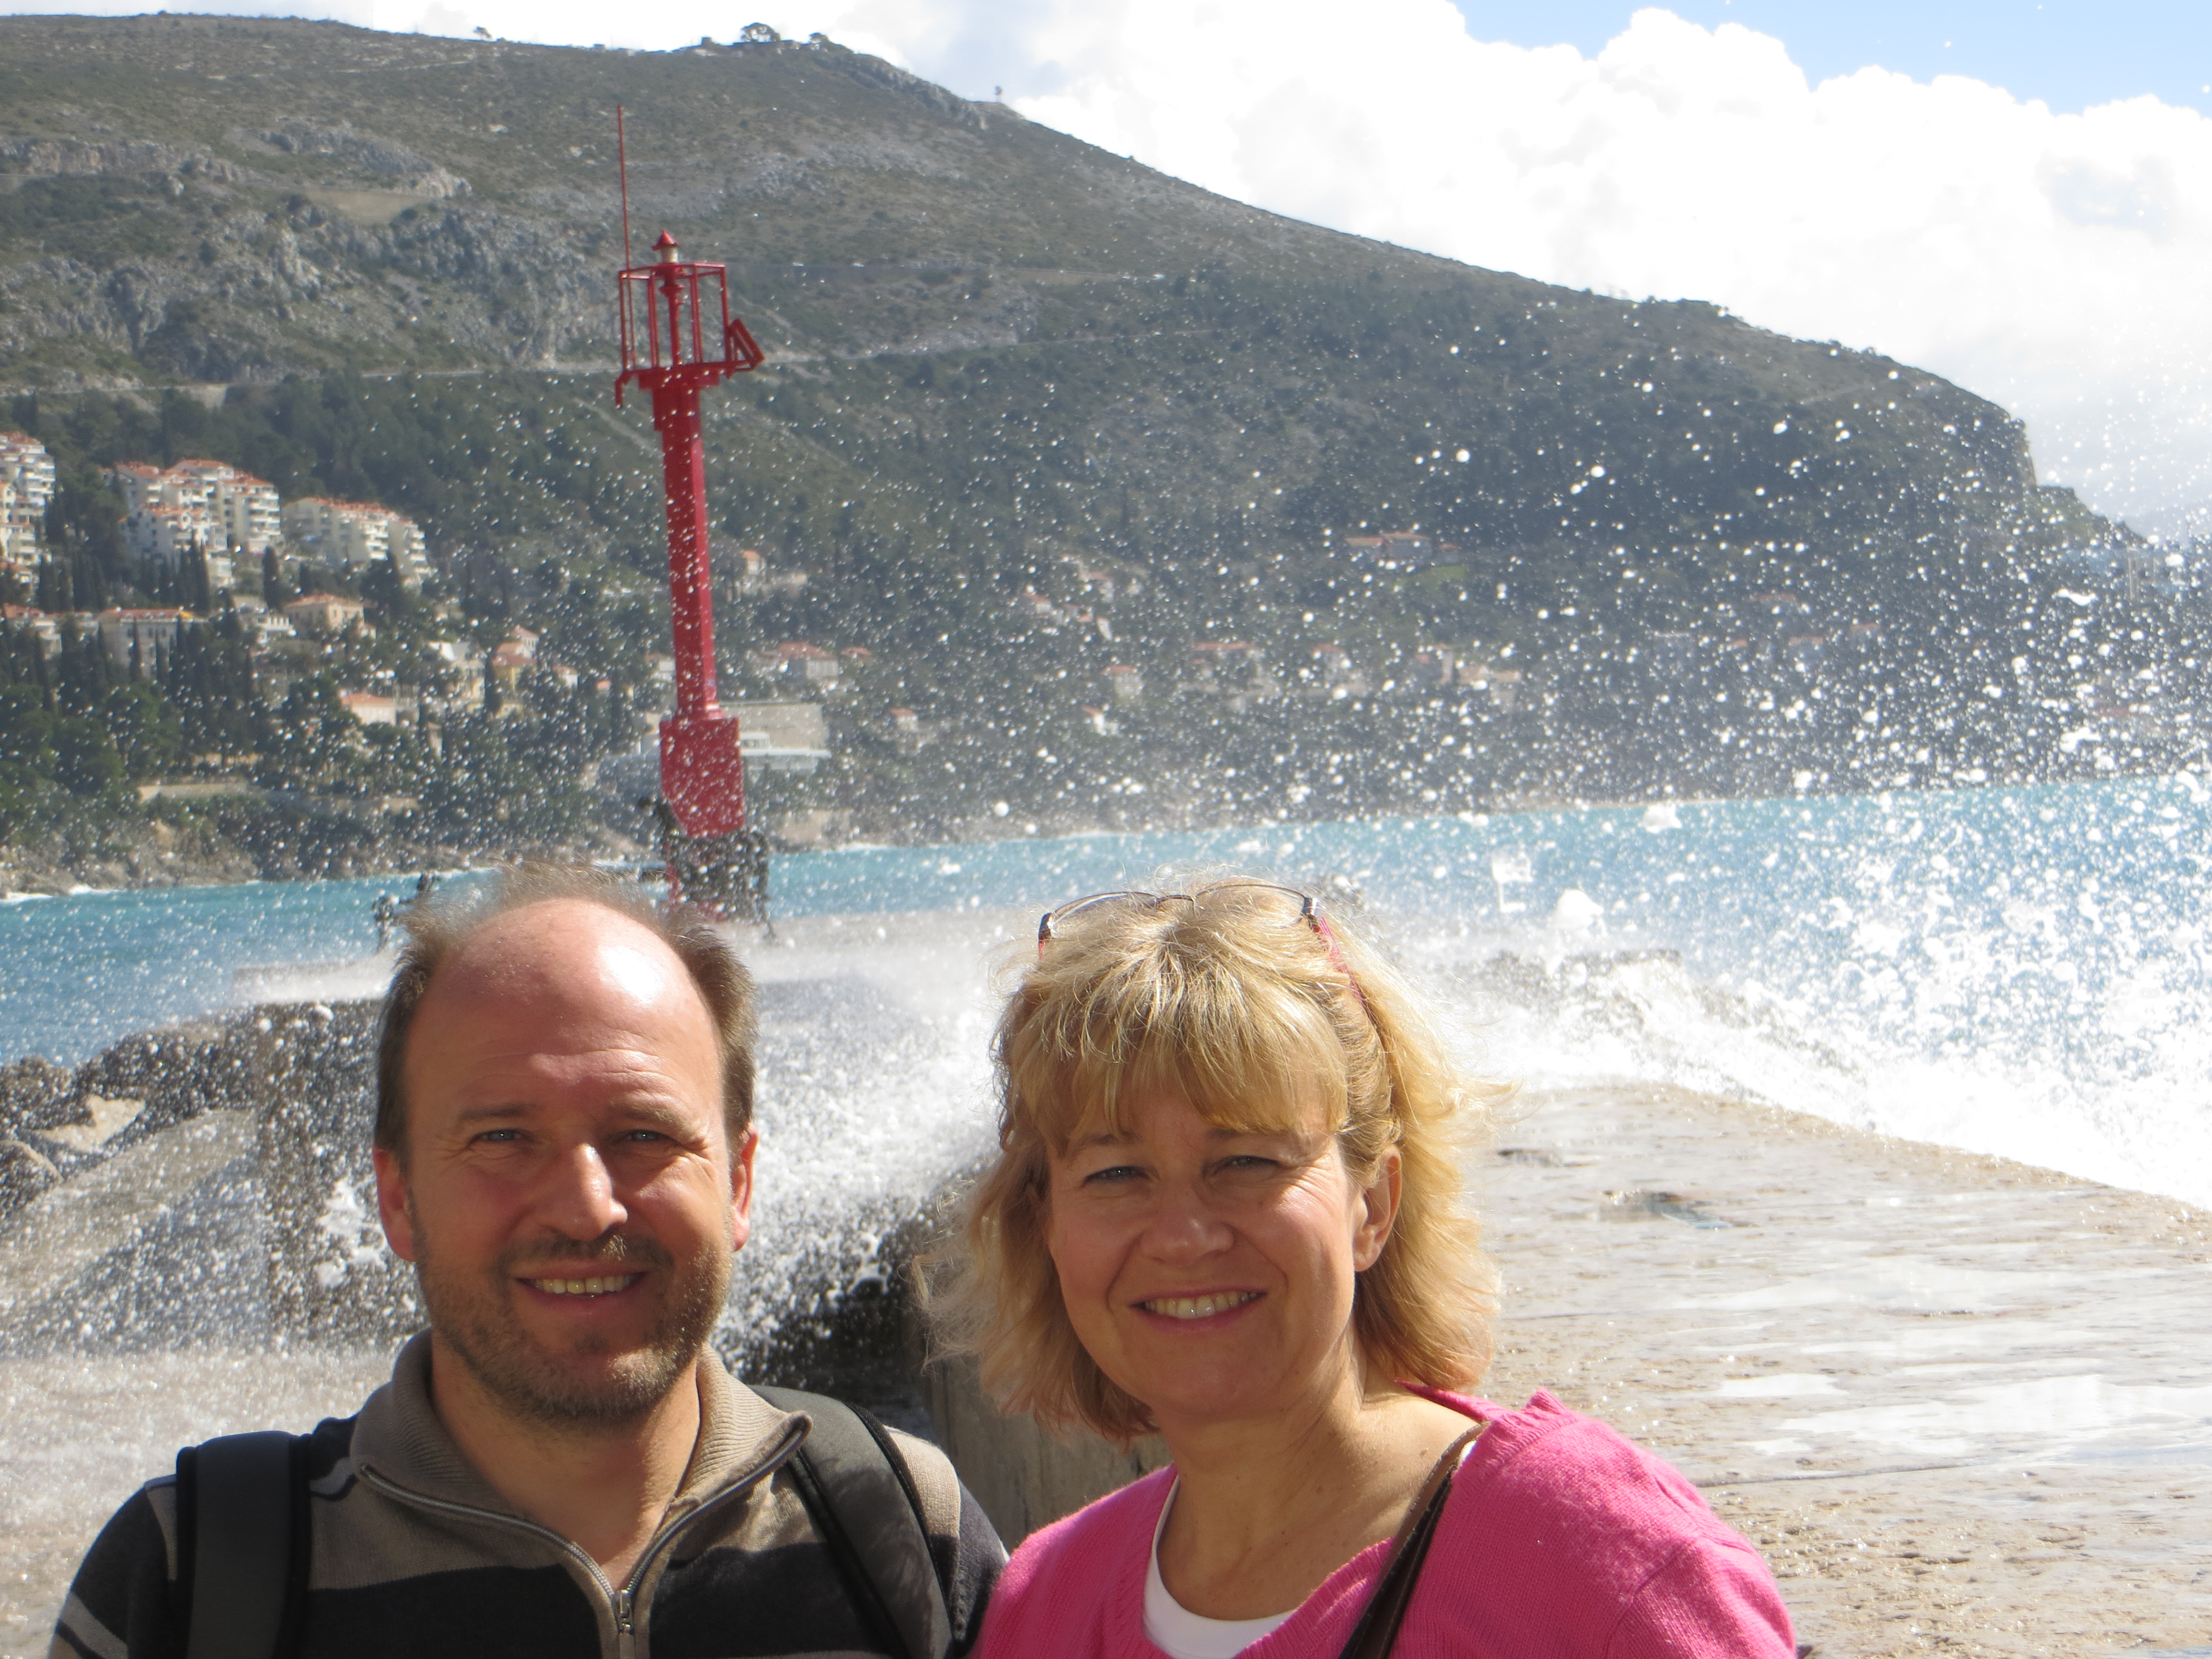
\includegraphics[width=\linewidth]{images/IMG_1216}
\captionof*{figure}{Frank und Angelika Bosch}
%\end{wrapfigure}
\end{center}
\textbf{Susanne Stoehr} Die Künstlerin Susanne Stoehr ist Mitarbeiterin der DMG in Italien. Sie schreibt: “Während einer
längeren Krankheitszeit beschäftigte ich mich intensiv mit Gottes Wort. Im Versuch, das zu begreif-
en, was ich zu verstehen meinte, malte ich meine Eindrücke in Farben und schrieb sie in Worten
auf. Seit mehr als 10 Jahren entstehen immer neue Bilder und Texte. Sie sind ein Spiegel dessen,
was ich um mich, vor allem im Beobachten der Schöpfung, entdecke. Ich erlebe immer wieder, dass
Menschen sich in meinen Bildern und Texten tief innen wiederfinden, und berührt werden.”

\textit{}

%Sidro
\begin{center}
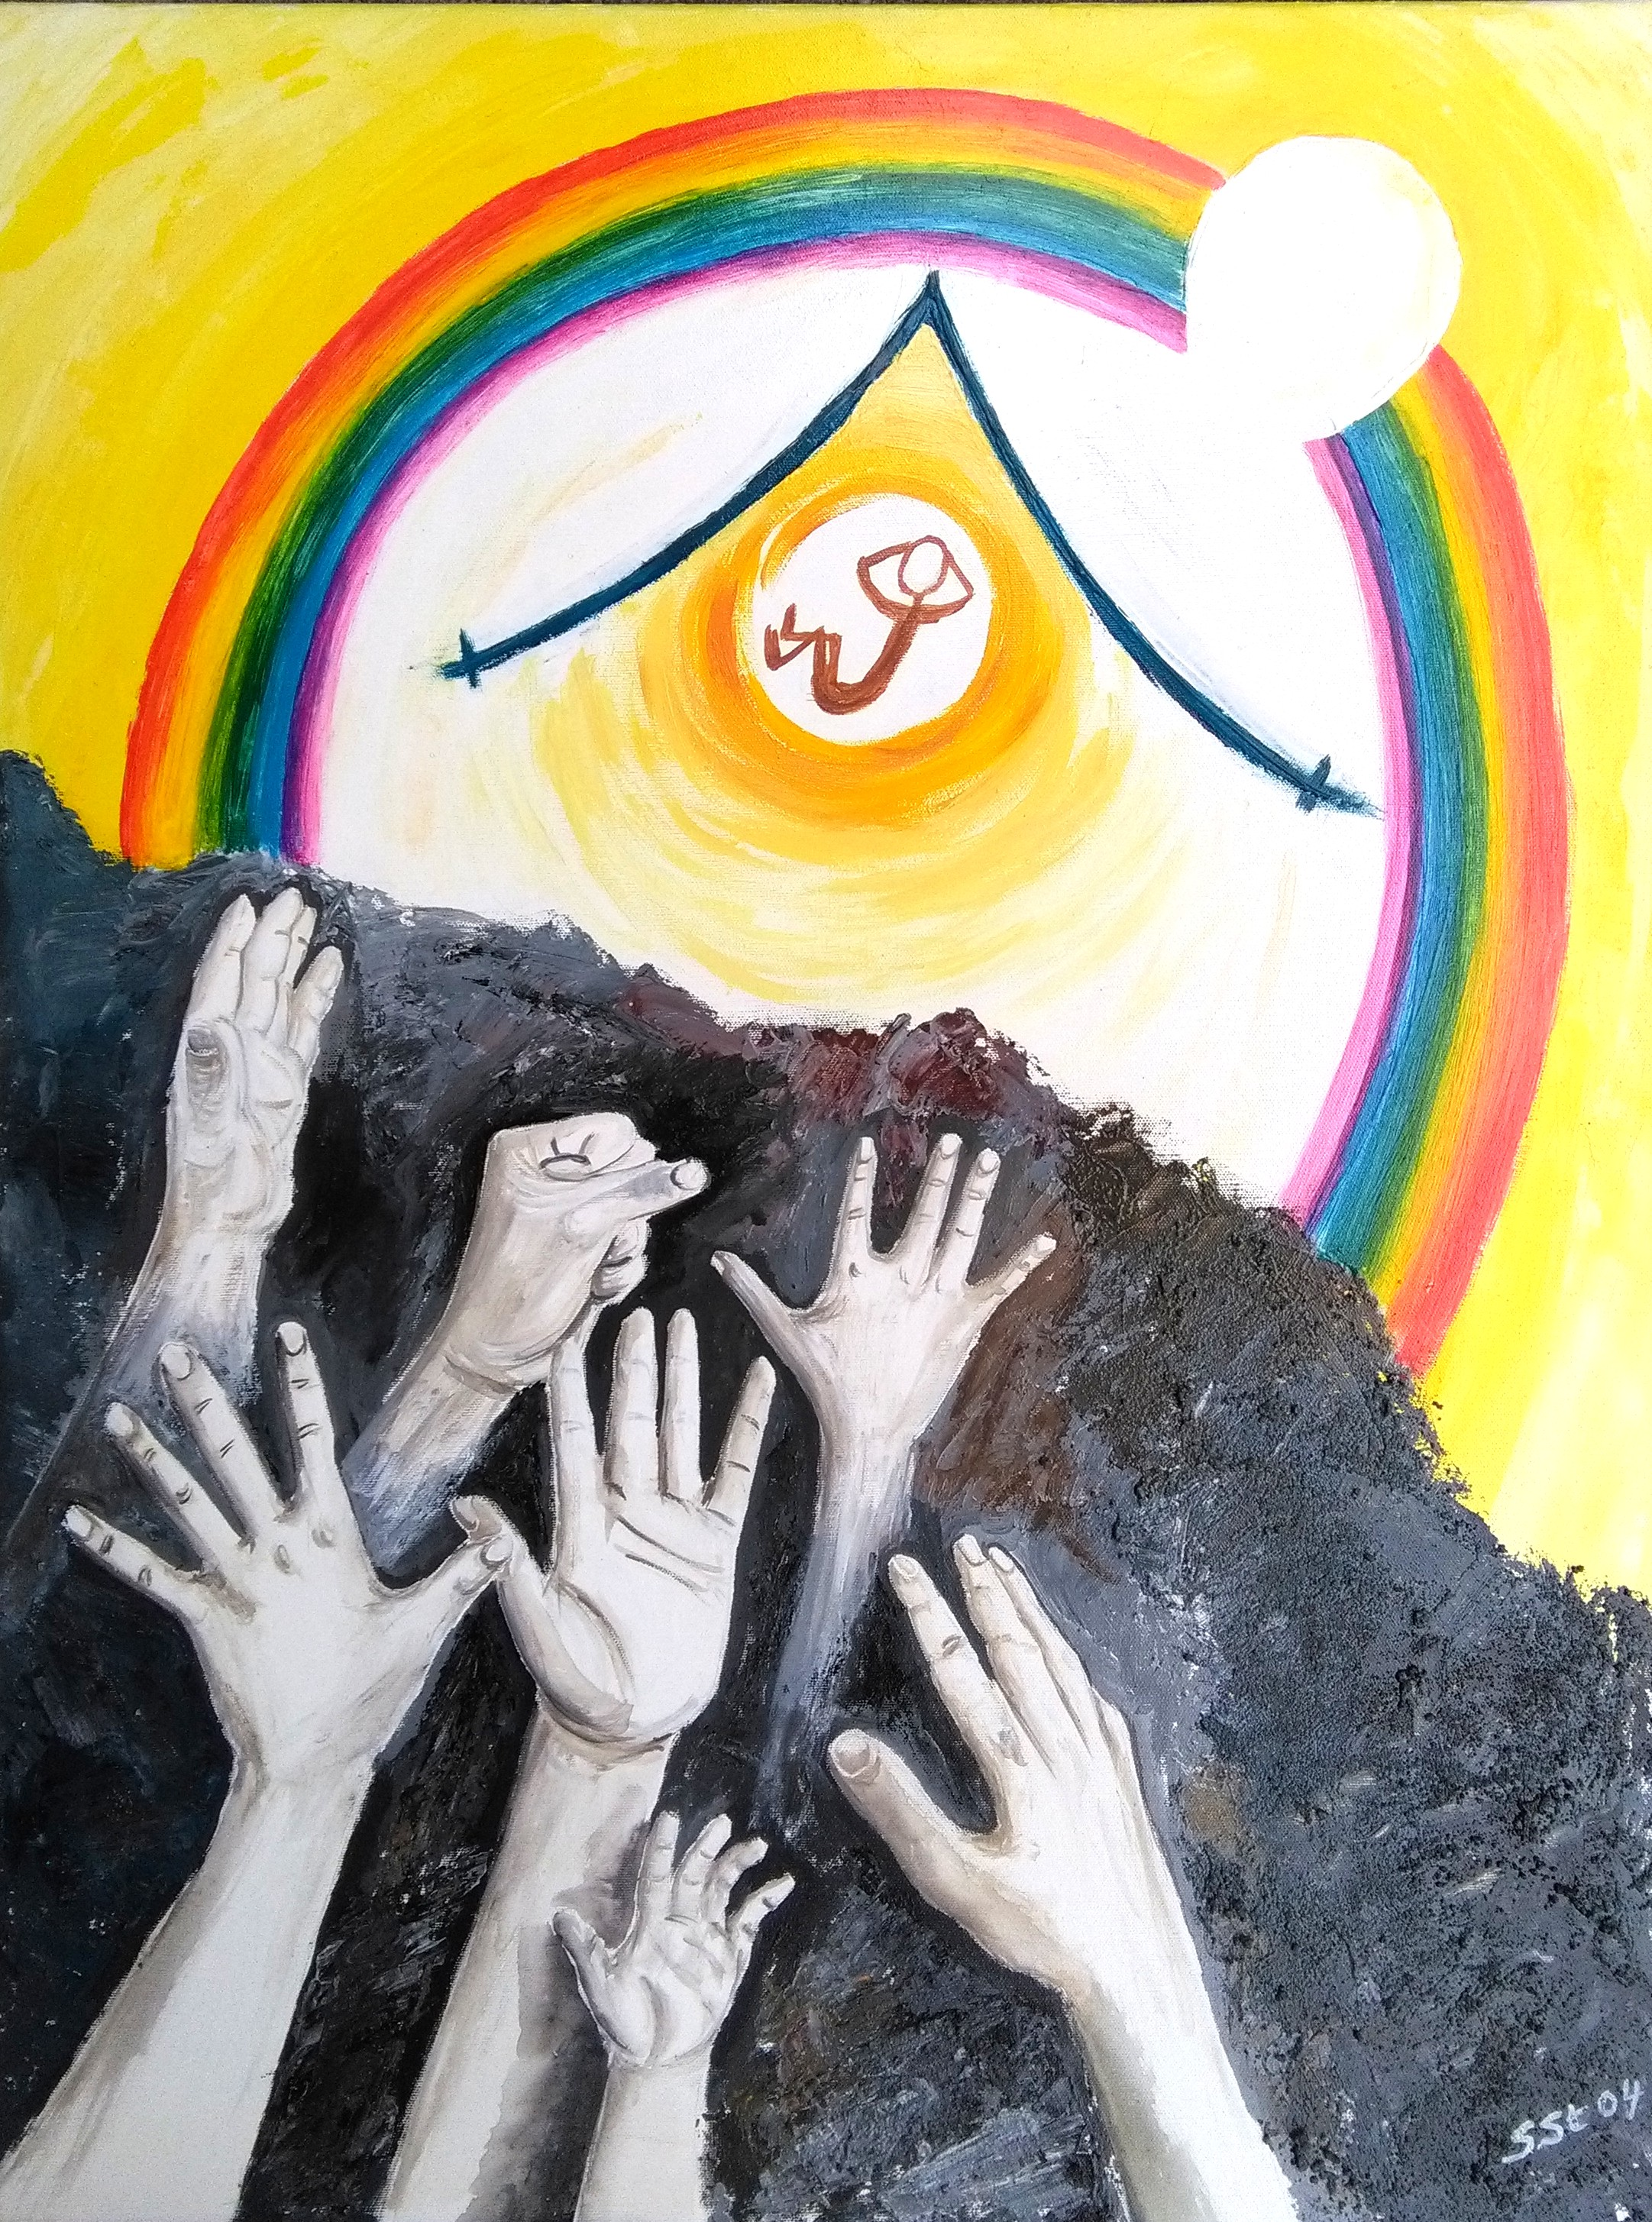
\includegraphics[width=\linewidth]{images/susanne/b2_derherristmeinlicht}
\captionof*{figure}{Die Bilder in diesem Liederbuch stammen von den Künstlern Susanne Stoehr und Mihovil Dorotić}
\end{center}

\vfill

%Mihovil Dorotić
%\begin{wrapfigure}{l}{1\linewidth}
\begin{center}
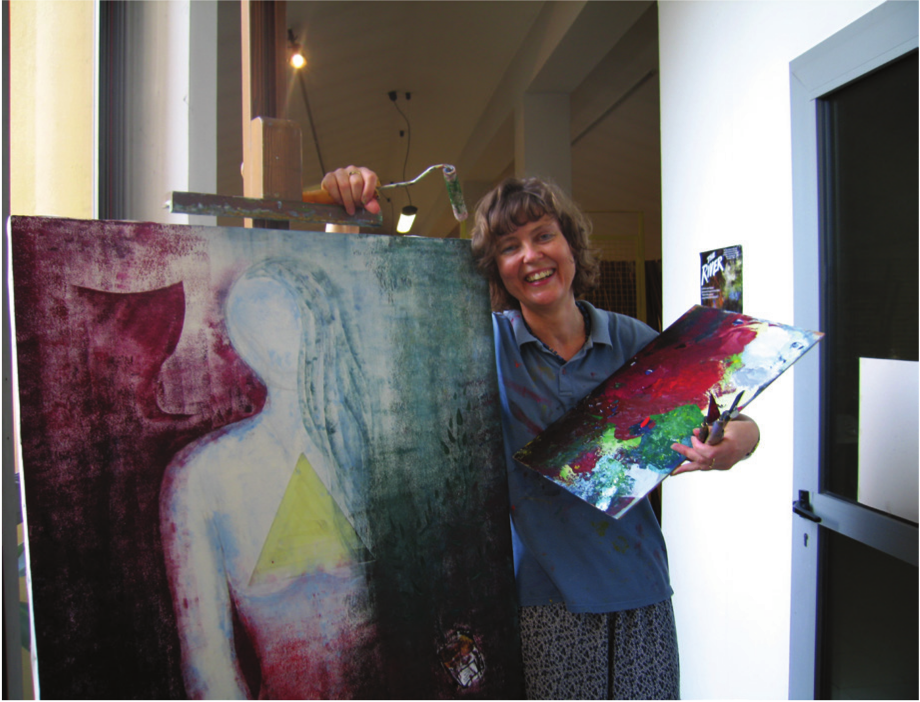
\includegraphics[width=\linewidth]{images/susanne}
\captionof*{figure}{Susanne Stoehr, Via Matteotti 6, 20846 Macerio/MB, Italia, E-mail: susanne.stoehr@gmail.com}
\end{center}

%\end{wrapfigure}


        \end{justify}
     \end{onehalfspacing}
\end{multicols}


%=========================================
%   SURADNICI I DRAGI PRIJATELJI
%=========================================
\newpage
\begin{multicols}{2}

    \begin{onehalfspacing}
        \begin{justify}
Die Lieder meiner CD’s werden von Chören, Kindergruppen und Gemeinden gesungen. Ich ver-
wende sie in meiner Arbeit in Kroatien für Kinderchöre, Freizeiten, Familyshows mit Clowns, Auf-
tritte in Heimen, Kindergärten, Krankenhäusern, Gemeinden usw.
Rückmeldungen wie die folgenden freuen mich sehr:
„Frank, eure Musik ist super!“ - „Von Herzen danke für die schöne Hymne zu unserer Freizeit, die
wir so fröhlich miteinander singen.“ - „Ich freue mich so, wenn ich bei euren Liedern mitsinge.“ -
„Danke. Ihr habt die besten Songs der Welt!“

%Frank i Angelika
%\begin{wrapfigure}{L}{1\linewidth}
\begin{center}
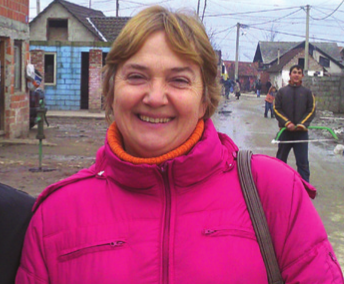
\includegraphics[width=\linewidth]{images/karmen}
\captionof*{figure}{Karmen Horvat}
%\end{wrapfigure}
\end{center}
Ich arbeite hier mit ganz tollen Leuten zusammen, von denen ich so viel lerne,
die mich total motivieren, begeistern und inspirieren. Sie sind mir liebe Freun-
de geworden. Es sind zu viele, um sie alle aufzuzählen, aber Karmen Horvat
und ihre Jungs von Octoberlight, Tomislav Tuškan mit Familie, sowie Mario
Colic mit Familie und
meine Clownkollegen
Rujana, Tonček und
Daniel möchte ich
doch nennen.
Besonders gerne singe
ich die Lieder mit den
Romakindern auf Freizeiten, bei regelmäßi-
gen Chorstunden und Auftritten in ihren
Dörfern und auf Romakonferenzen. Diese
Kinder erleben viel Leid. Das Leben ihrer
Familien ist geprägt von Arbeitslosigkeit,
Drogen, Gewalt, Schmutz und Alkohol.
Mädchen werden oft bereits im Alter von
12 oder 13 Jahren verheiratet und sind bald
darauf schwanger. Dann schmeißen sie die
Schule. Wir möchten die Kinder und ihre
Familien für ein Leben mit Jesus begeistern,
unter anderem durch das Singen dieser Lieder
Wenn sich ein Roma für Jesus entscheidet,
dann erkennen nicht nur wir es – dann verändert sich sein Leben – und das ist offensichtlich für das
ganze Dorf.\\
\textit{}

\begin{center}
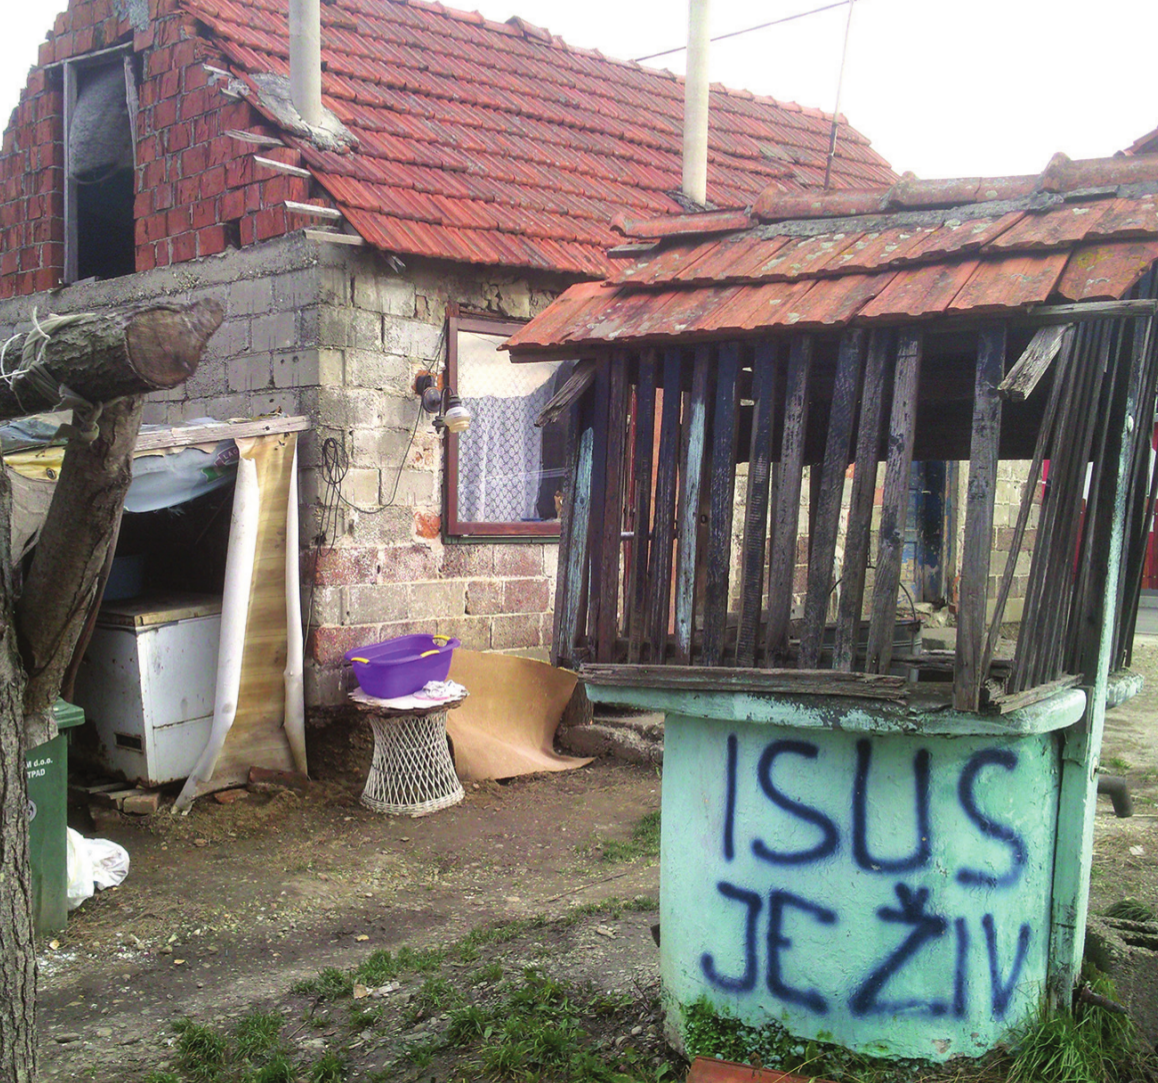
\includegraphics[width=\linewidth]{images/cigo}
\captionof*{figure}{Auf diesem Brunnen im Romadorf steht: “Jesus lebt”.}
\end{center}

\begin{center}
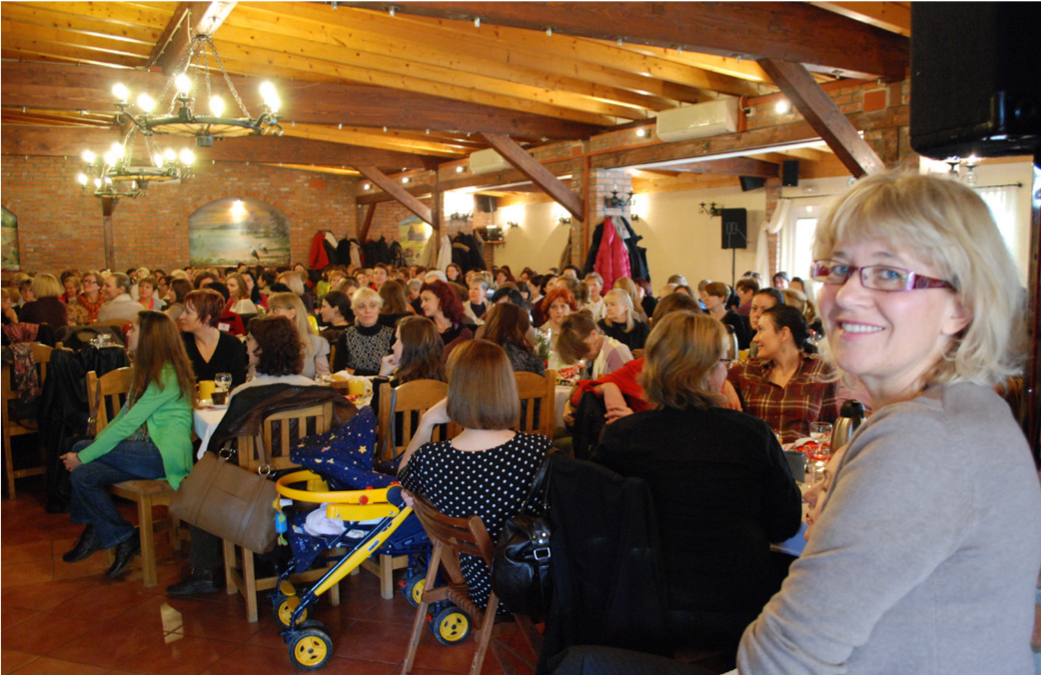
\includegraphics[width=\linewidth]{images/dorucakzazene}
\captionof*{figure}{Meine Frau Angelika ist Koordinatorin der Frauen-
frühstücksarbeit in Kroatien.
www.dorucak-za-zene.com}
\end{center}

Unter www.mjuzikids.de gibt es weitere Informa-
tionen zu unserer Arbeit.

\vfill

\begin{center}

\includegraphics[width=0.5\linewidth]{images/DMG_2014}
\captionof*{figure}{Wir leben mit unseren 3 Kindern seit Februar 2000 in Zagreb und sind durch DMG interpersonal e.V. entsandt | www.DMGint.de}
\end{center}

%\end{wrapfigure}


        \end{justify}
     \end{onehalfspacing}
\end{multicols}
%=========================================
%   PASTORALNI
%=========================================
\newpage
\begin{center}
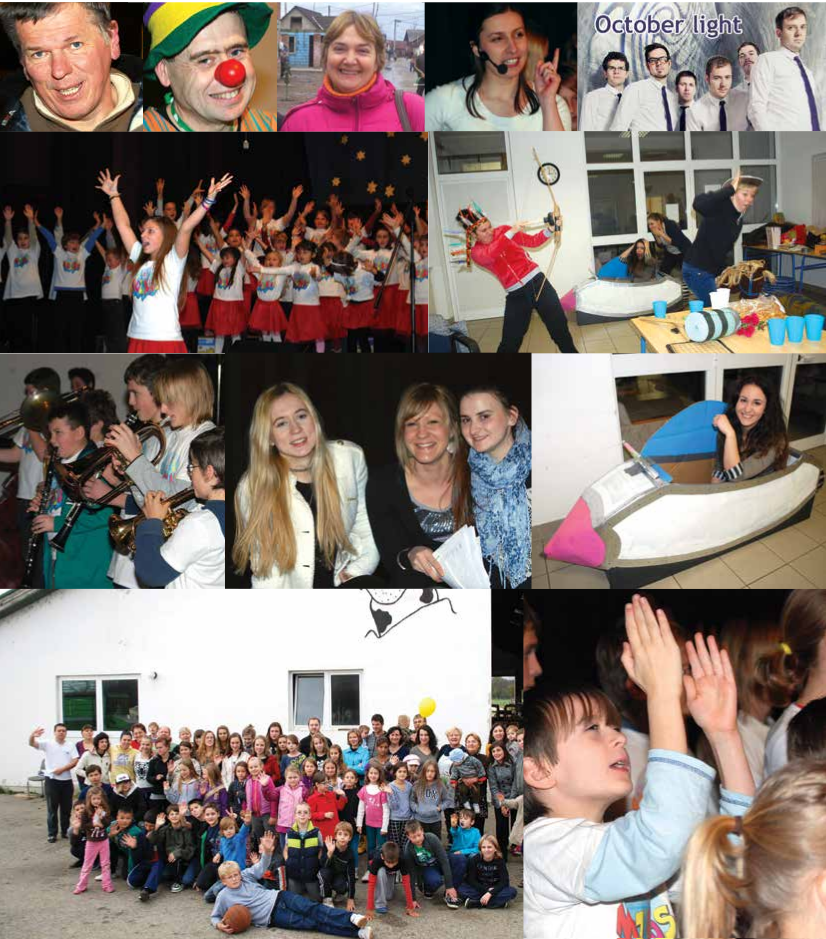
\includegraphics[width=\linewidth]{images/suradnici}\\

\vfill

\end{center}

\newpage
\begin{center}
Unsere Arbeit in Kroatien ist möglich dank vieler kleinerer und größerer Spenden. Jeder noch so
kleine Betrag hilft uns und macht unsere Musikarbeit möglich.\\
\vspace*{0.2cm}
\textbf{Spendenkonten:}\\
\vspace*{0.1cm}
Deutschland:\\
Volksbank Kraichgau, IBAN: DE02 6729 2200 0000 2692 04\\
BIC: GENODE61WIE (Vermerk: Familie Bosch)\\
\vspace*{0.2cm}
Schweiz:\\
PC (Kto-Inhaber SMG) Nr. 80-42881-3 mit Vermerk: DMG (Familie Bosch)\\
IBAN: CH92 0900 0000 8004 2881 3\\
BIC: POFICHBEXXX\\
\vspace*{1cm}
Wenn Sie unsere Arbeit näher kennenlernen möchten, senden wir Ihnen gerne
halbjährlich unseren Informationsbrief zu.\\
Frank und Angelika Bosch, Grigora Viteza 2, HR-10090 Zagreb, Kroatien\\
Tel.: +385 1 3435 420\\
Mail: angelika.bosch@gmail.com | frank.bosch.zagreb@gmail.com\\
mjuzikids@gmail.com

\vfill
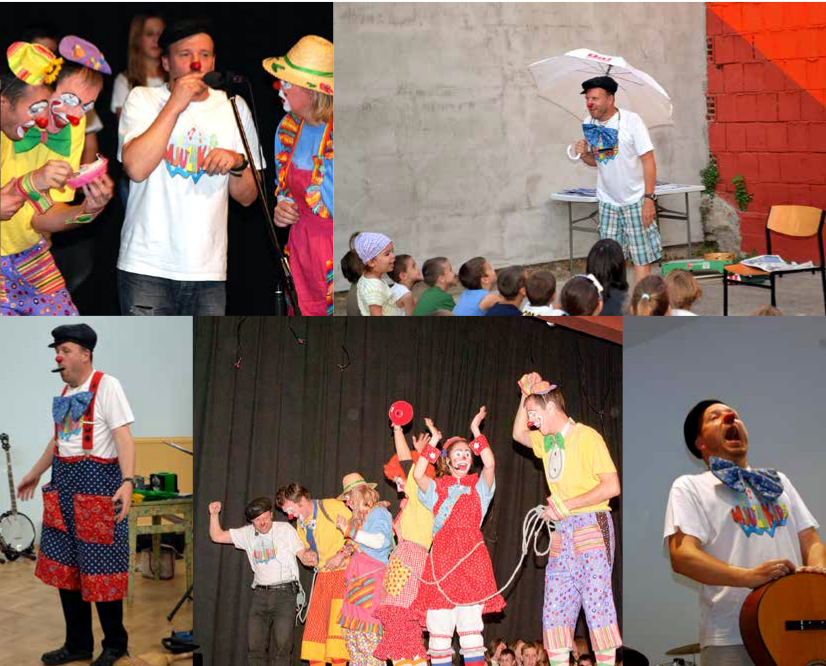
\includegraphics[width=\linewidth]{images/klauni}\\

\end{center}

%=========================================
%   PJESME
%=========================================
%pjesma 1
\newpage
\phantomsection
\begin{minipage}[b]{0.5\linewidth}
\addcontentsline{toc}{section}{\texorpdfstring{{\rednifont\doccolor1.}\hspace{\onedigitspacing}}{}GEDANKEN DES FRIEDENS \ttfamily(Jer 29,11)}
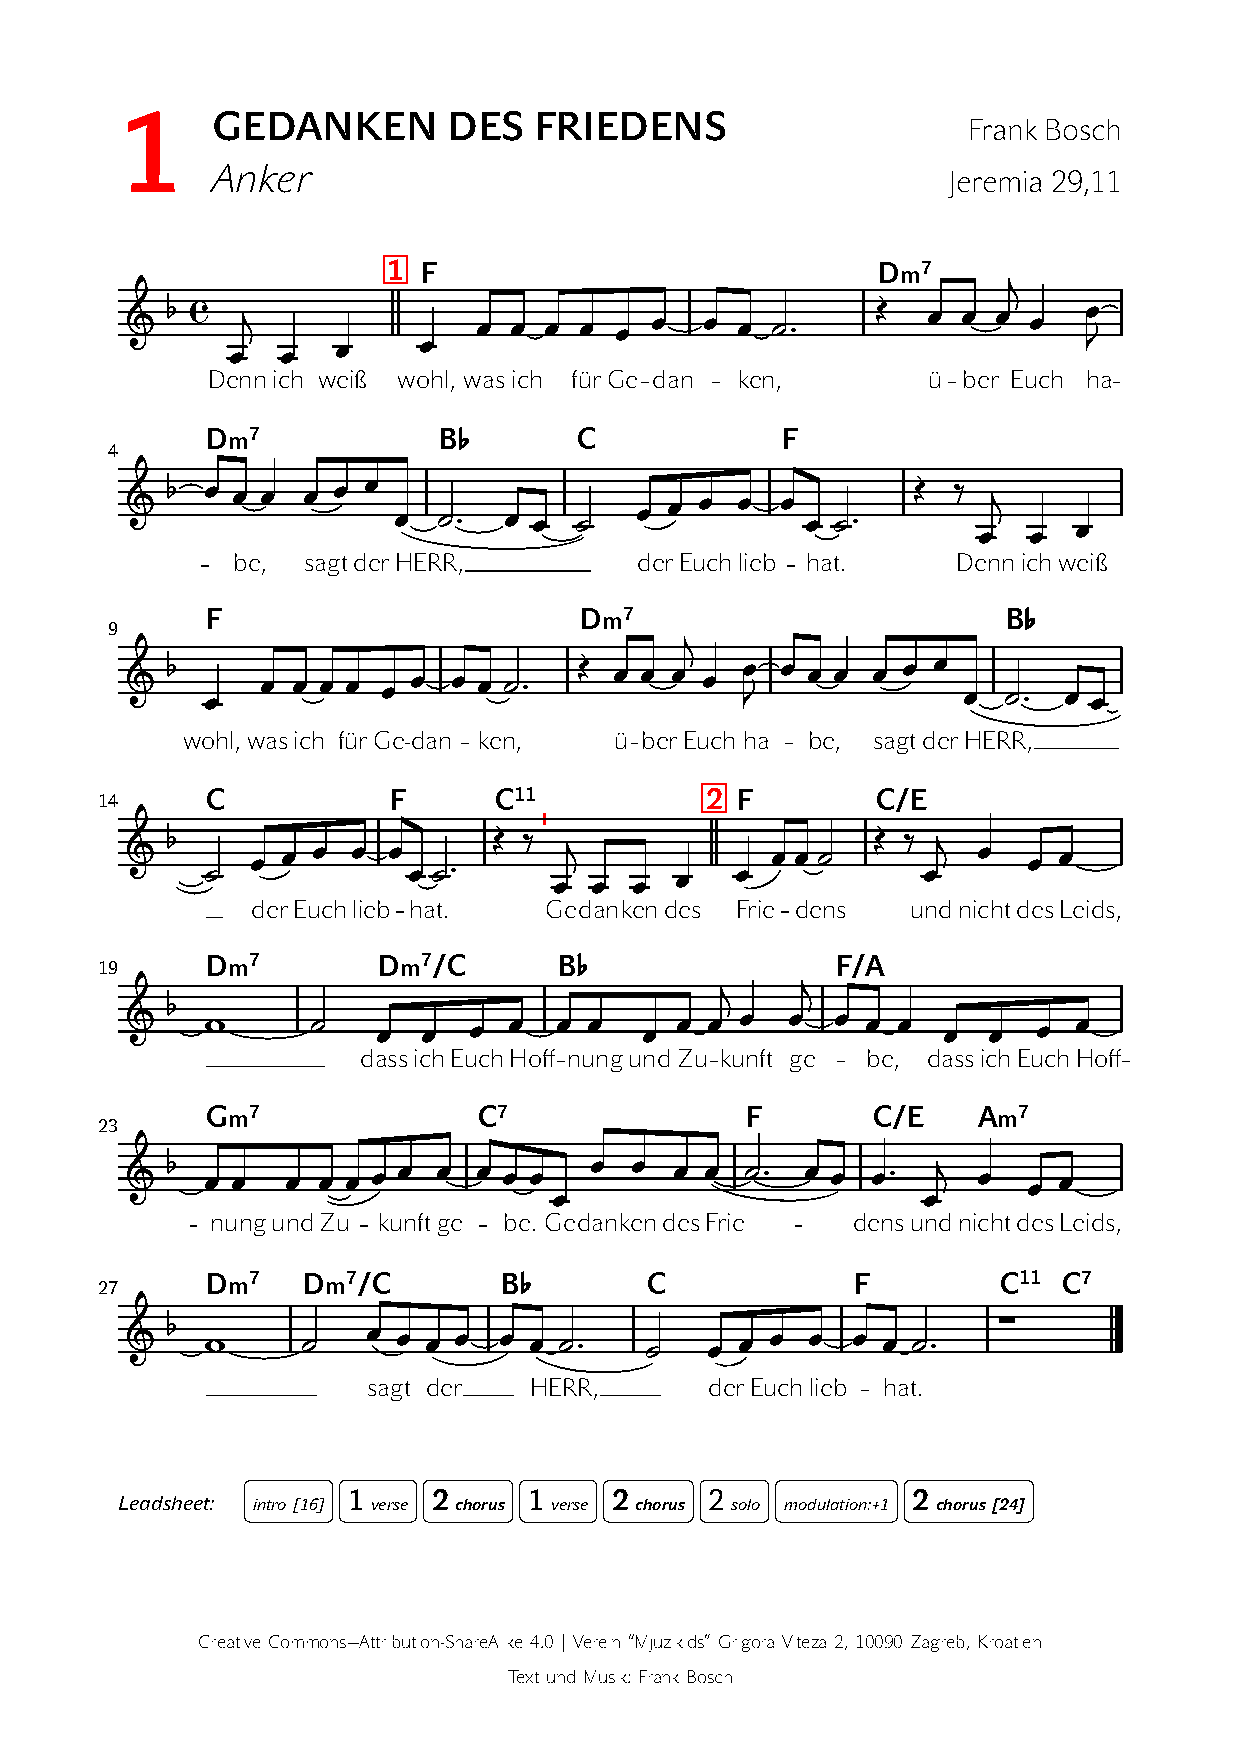
\includepdf[pages={1},noautoscale]{lilypond/de/src/01_gedanken_des_friedens.pdf}
\end{minipage}

\newpage
\begin{center}
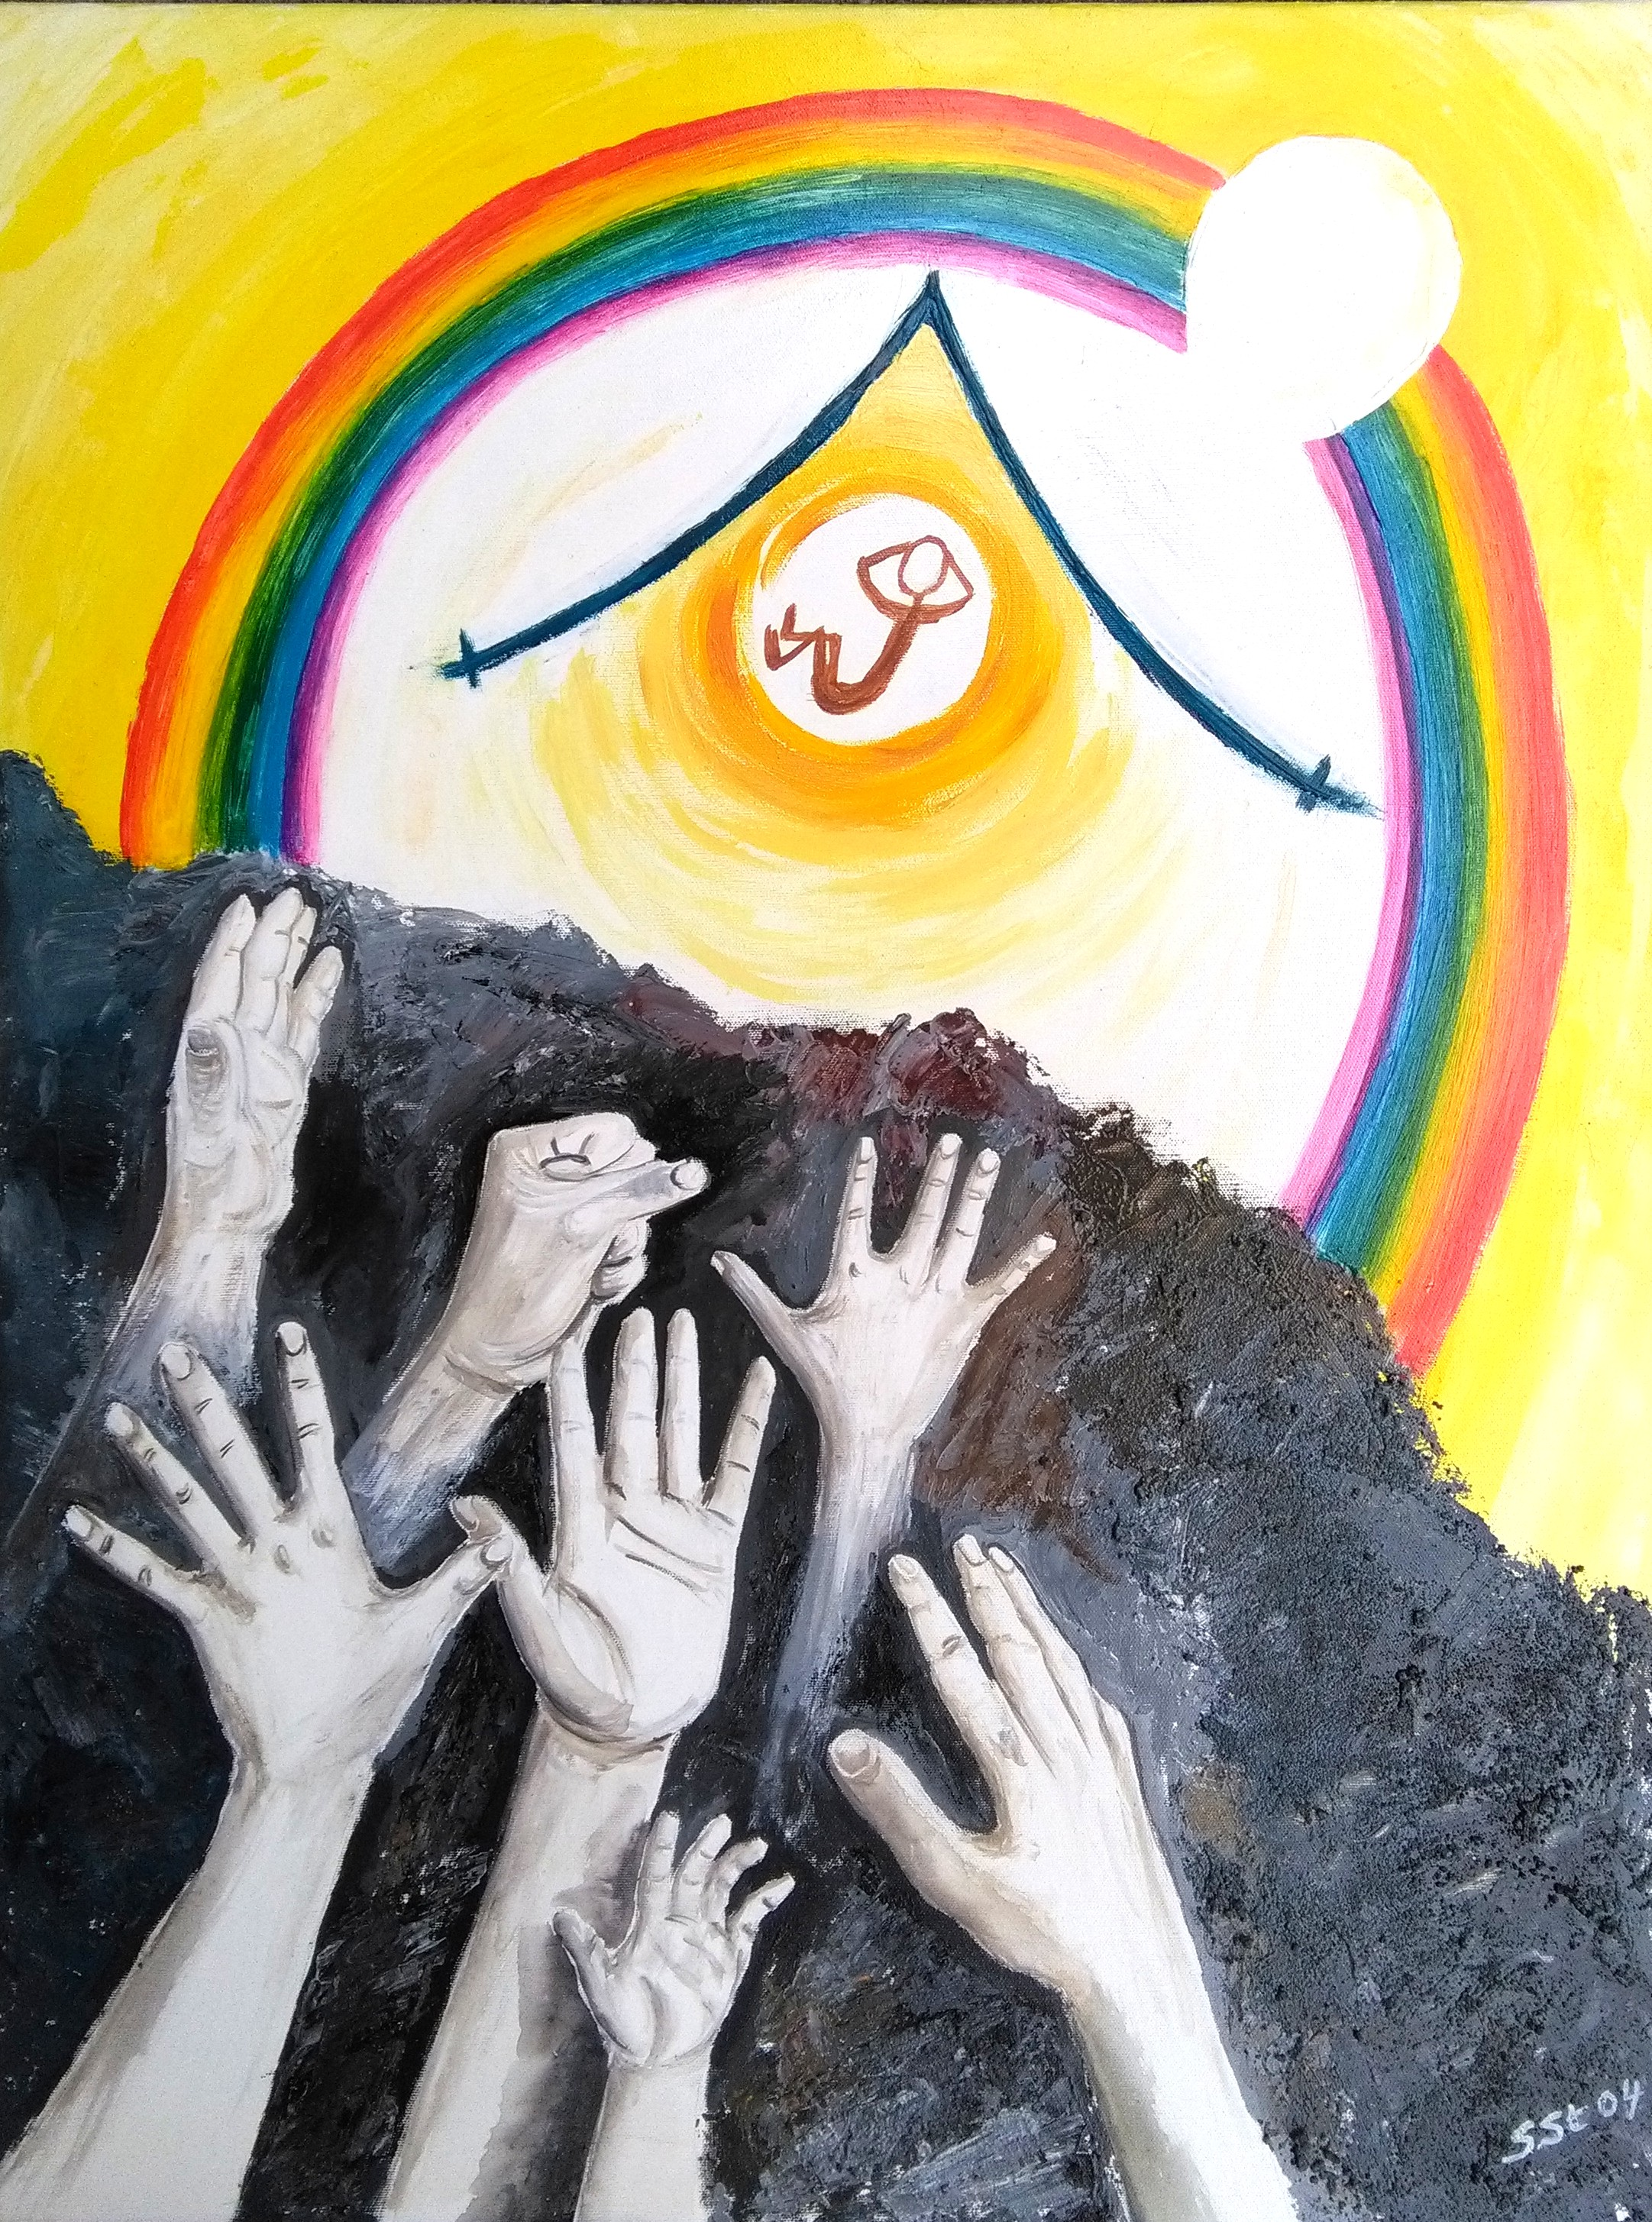
\includegraphics[width=\linewidth]{images/susanne/b2_derherristmeinlicht}
\end{center}

%pjesma 2
\newpage
\phantomsection
\begin{minipage}[b]{0.5\linewidth}
\addcontentsline{toc}{section}{\texorpdfstring{{\rednifont\doccolor2.}\hspace{\onedigitspacing}}{}DER HERR IST MEIN LICHT \ttfamily(Ps 27,1.4–5)}
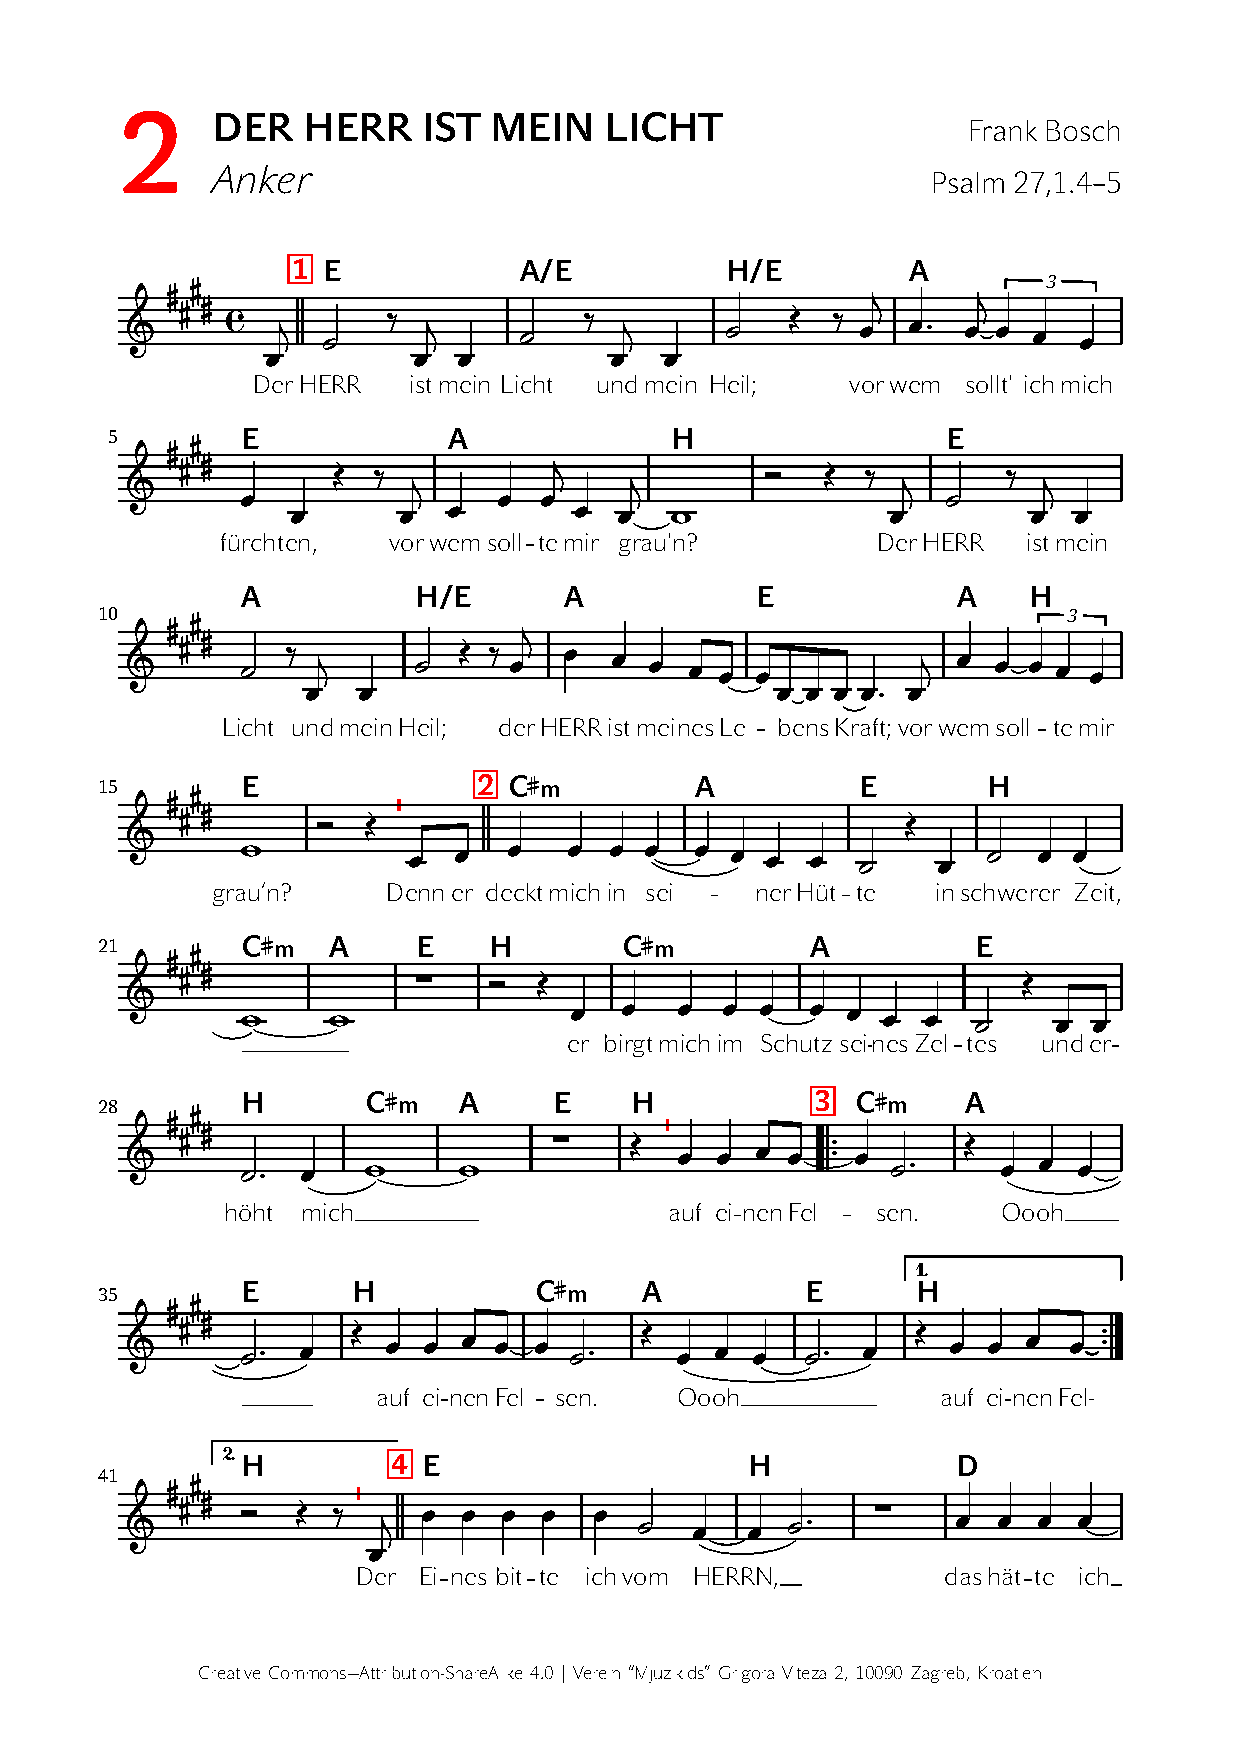
\includepdf[pages={1},noautoscale]{lilypond/de/src/02_der_herr_ist_mein_licht.pdf}
\end{minipage}

\newpage

\includepdf[pages={2},noautoscale, %
    picturecommand={\setlength\unitlength{1cm}%
         \put(2,5){\includegraphics[width=\linewidth,scale=1]{images/susanne/Lichtvertreibtdiedunkelheit}}}]%
         {lilypond/de/src/02_der_herr_ist_mein_licht.pdf}


%pjesma 3
\newpage
\phantomsection
\begin{minipage}[b]{0.5\linewidth}
\addcontentsline{toc}{section}{\texorpdfstring{{\rednifont\doccolor3.}\hspace{\onedigitspacing}}{}LICHT VERTREIBT DIE DUNKELHEIT \ttfamily(Jes 9,17.14)}
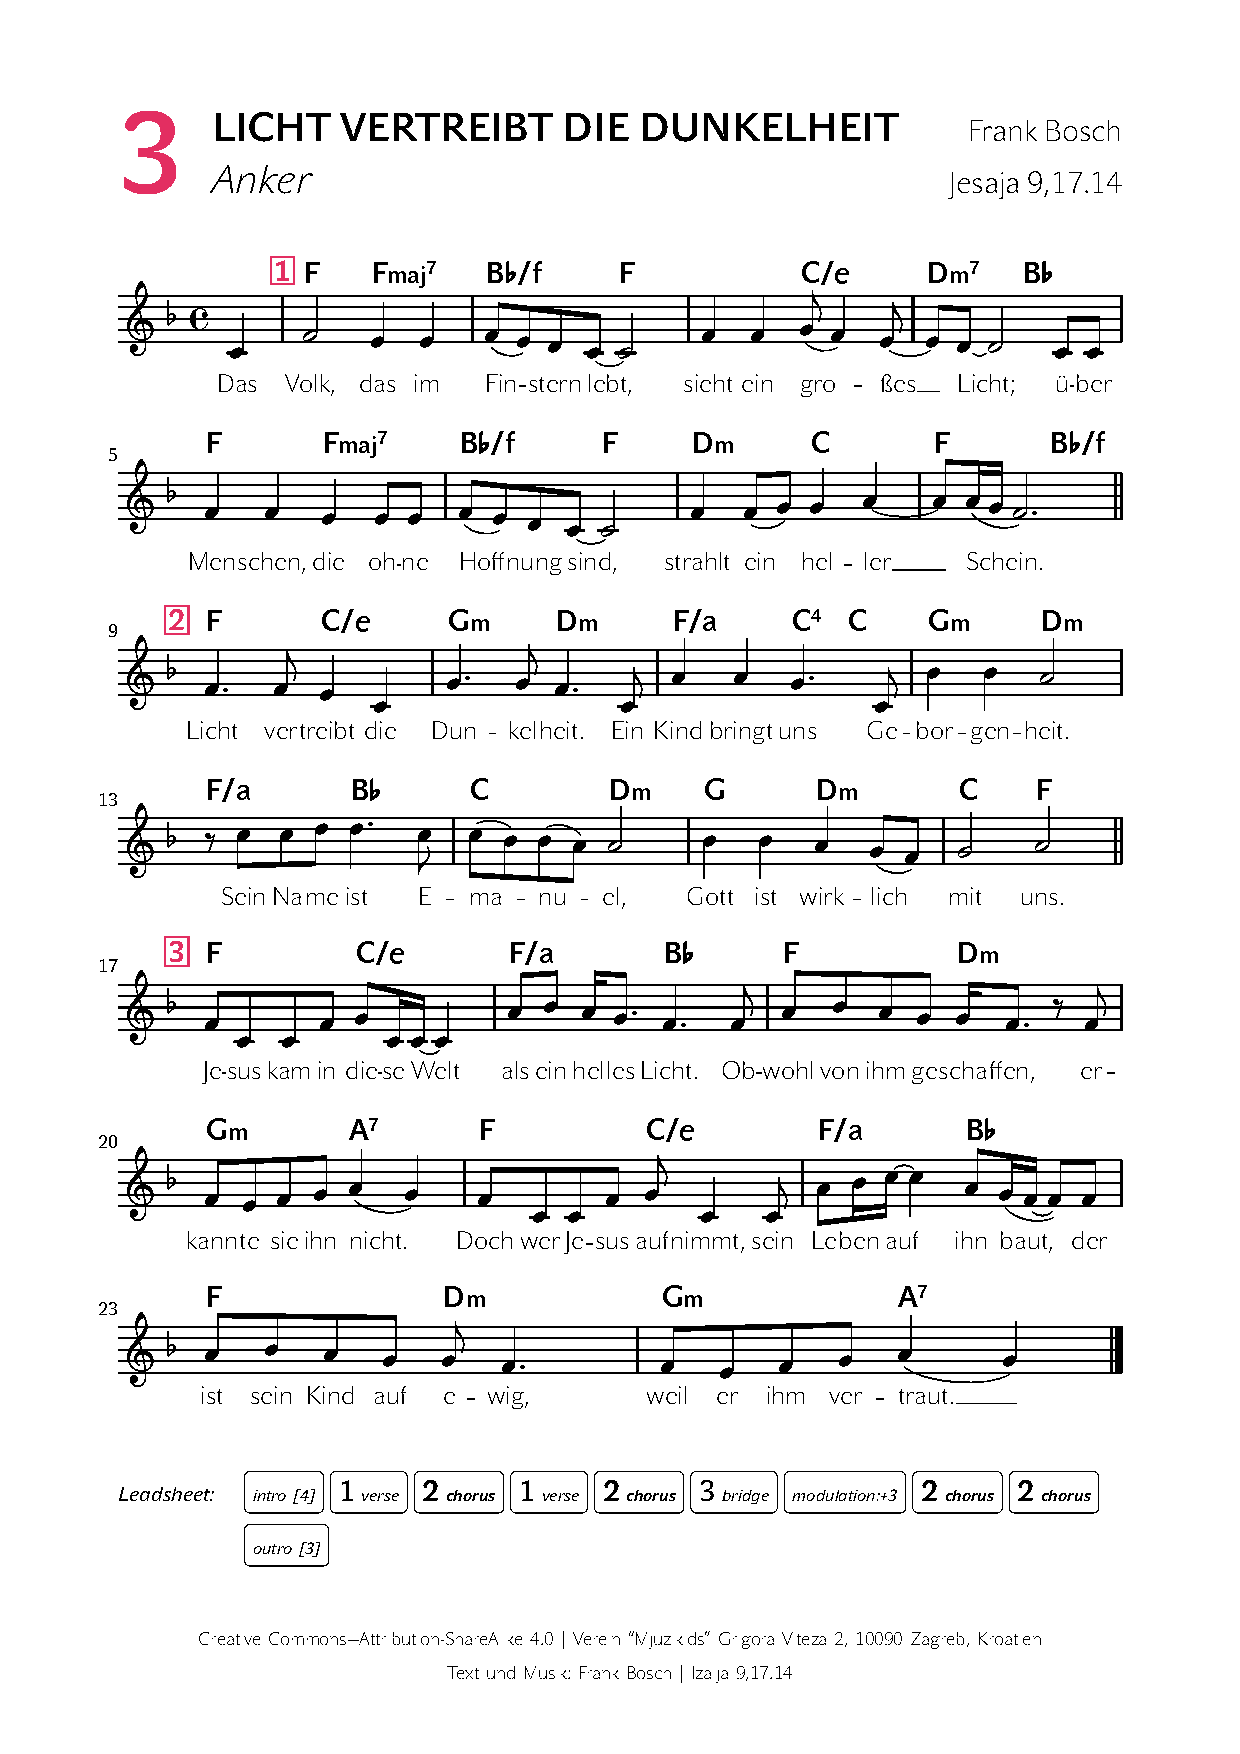
\includepdf[pages={1},noautoscale]{lilypond/de/src/03_licht_vertreibt_die_dunkelheit.pdf}
\end{minipage}

\newpage
\begin{center}
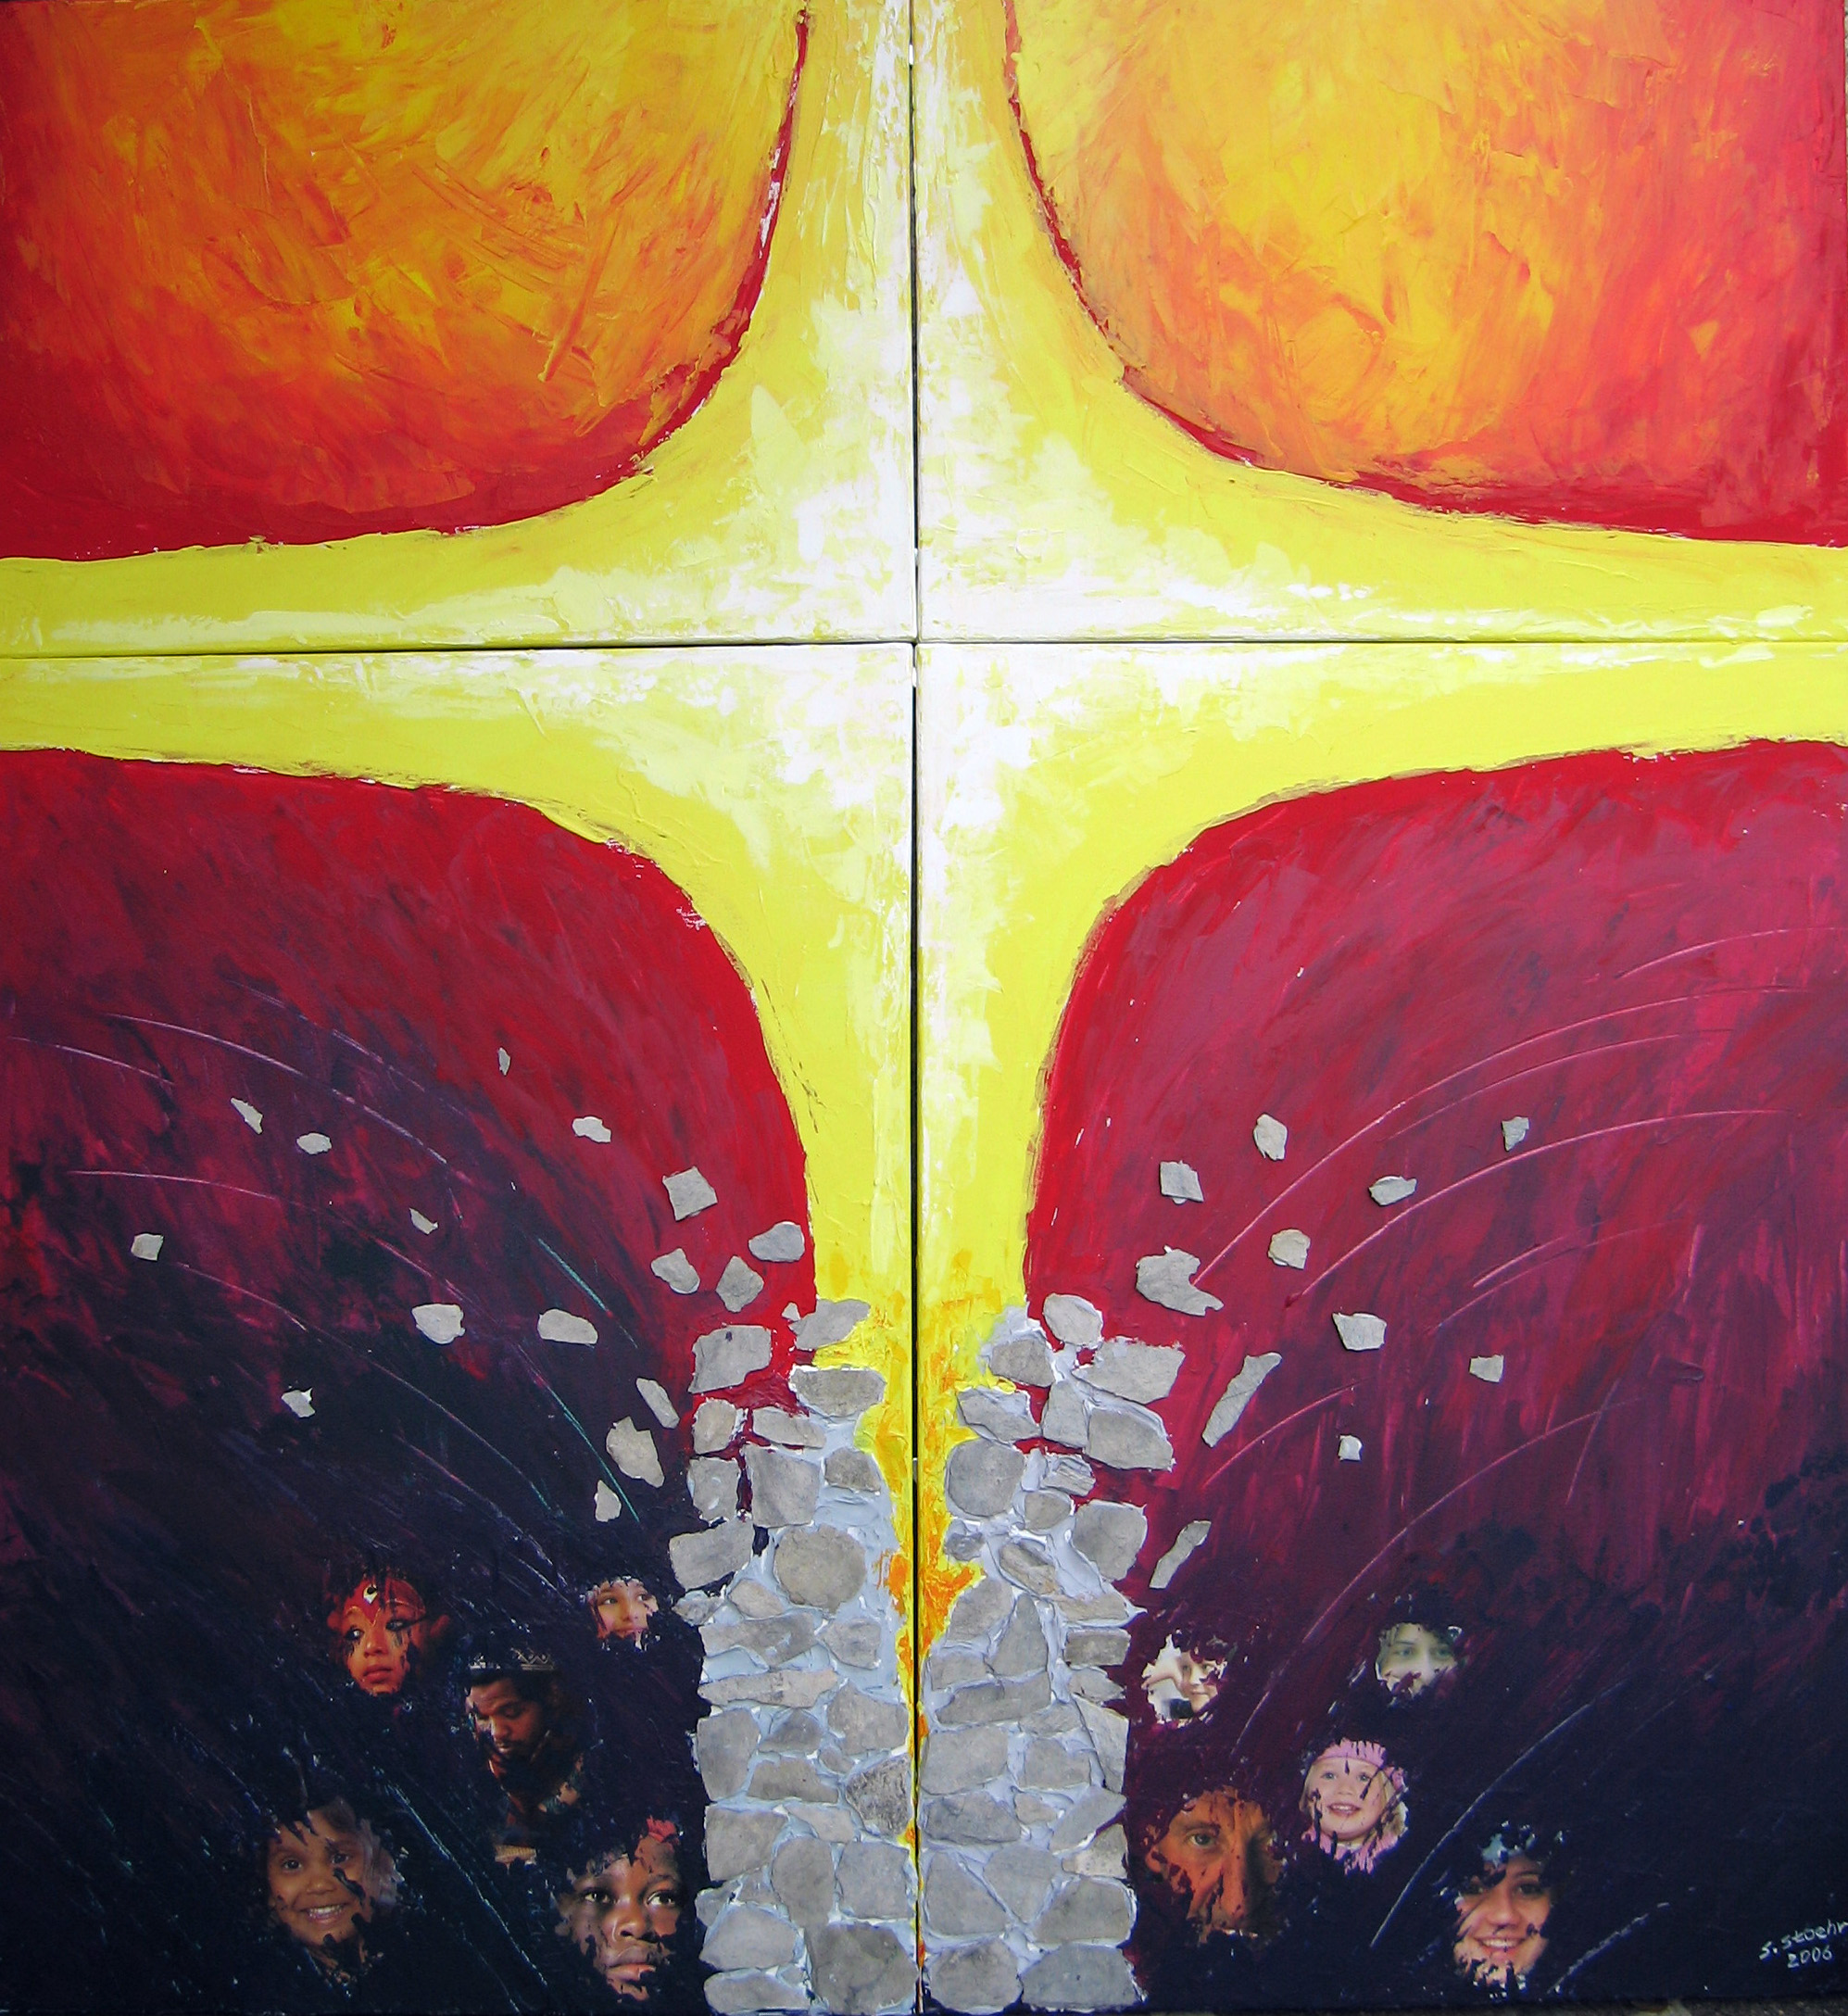
\includegraphics[width=\linewidth]{images/susanne/c3_lichtvertreibtdiedunkelheit}

\end{center}


%pjesma 4
\newpage
\phantomsection
\addcontentsline{toc}{section}{\texorpdfstring{{\rednifont\doccolor4.}\hspace{\onedigitspacing}}{}ICH ABER UND MEIN HAUS \ttfamily(Jos 24,15}
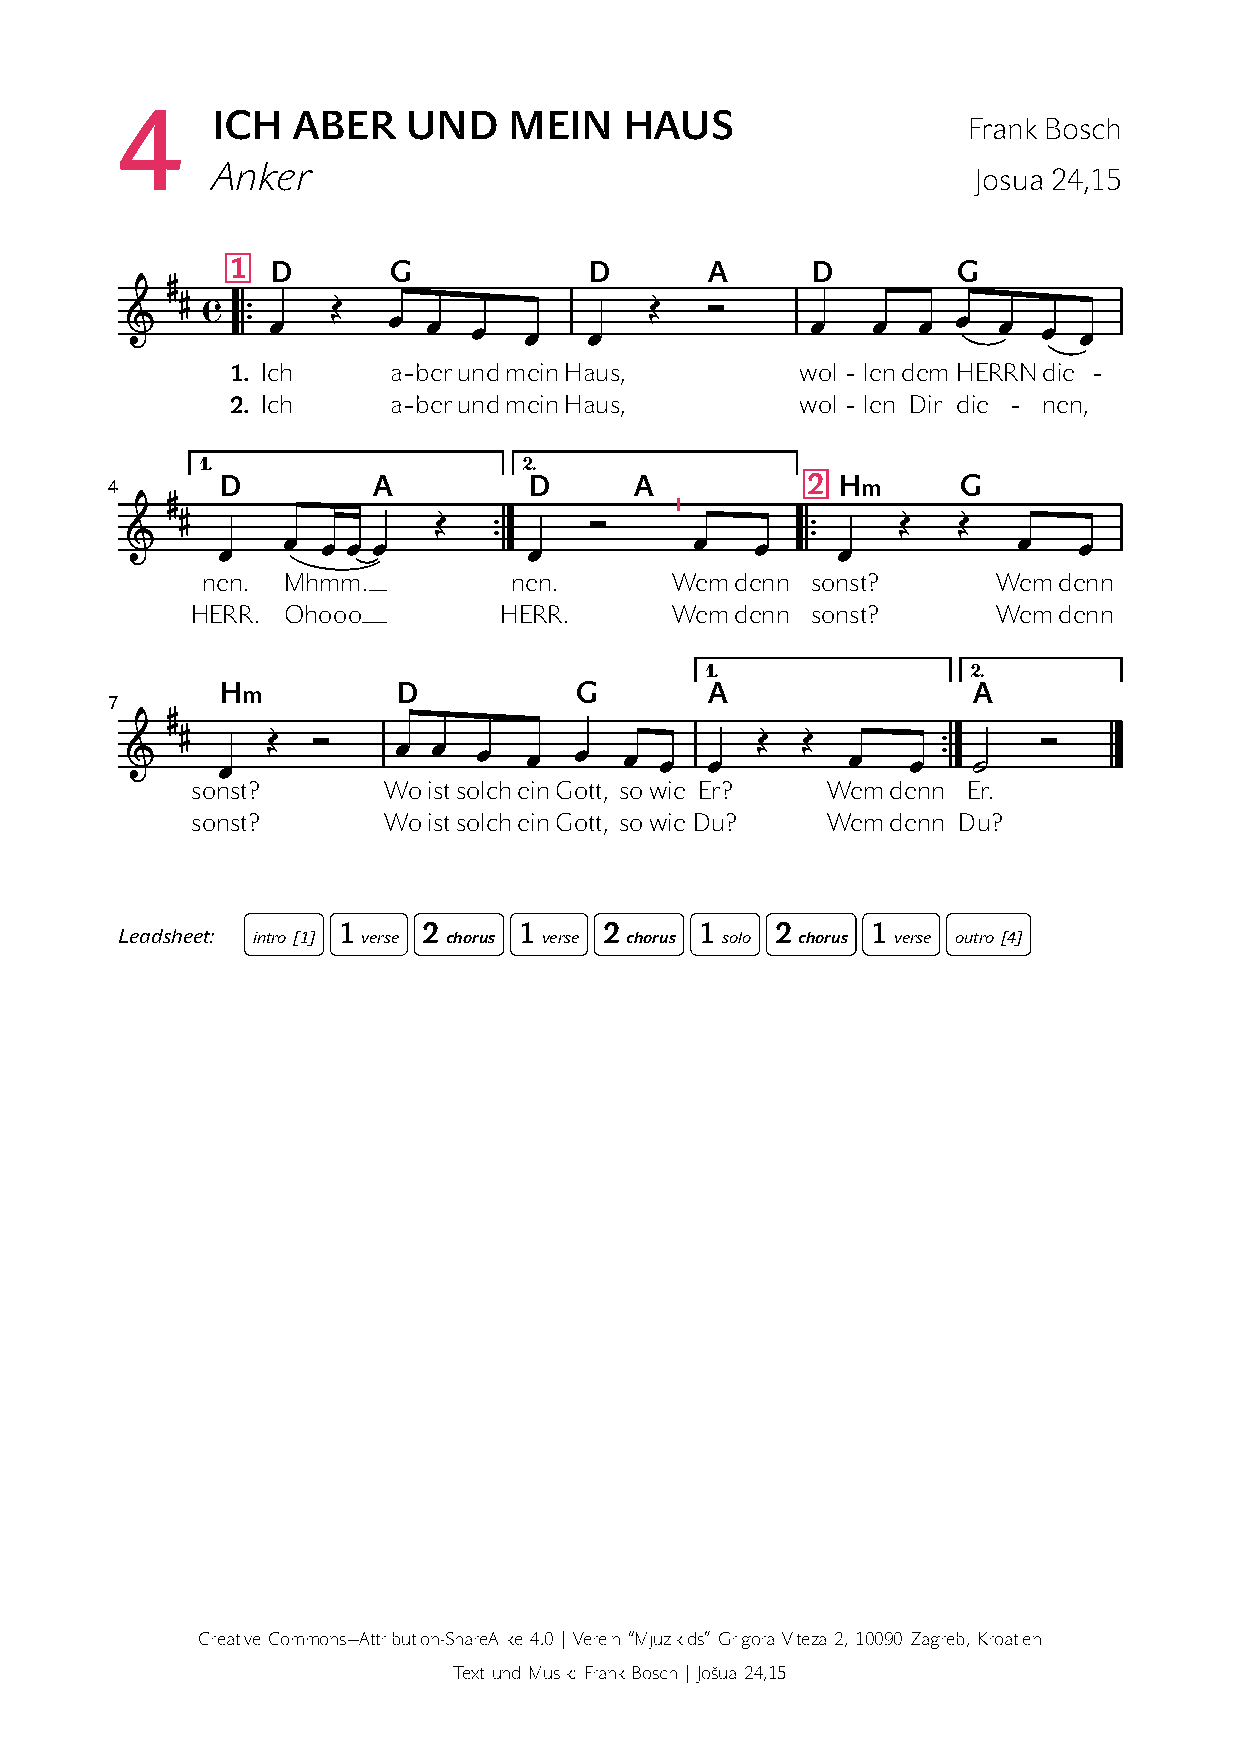
\includepdf[pages={1},noautoscale,]
         {lilypond/de/src/04_ich_und_mein_haus.pdf}

\newpage
\begin{center}
\includegraphics[width=\linewidth]{images/susanne/d4_ichundmeinhaus}
\end{center}

%pjesma 5
%Pokušaj uvrštavanja slike u sliku
\newpage
\phantomsection
\begin{minipage}[b]{0.5\linewidth}
\addcontentsline{toc}{section}{\texorpdfstring{{\rednifont\doccolor5.}\hspace{\onedigitspacing}}{}DENNOCH BLEIBE ICH STETS AN DIR \ttfamily(Ps 73,23–26)}
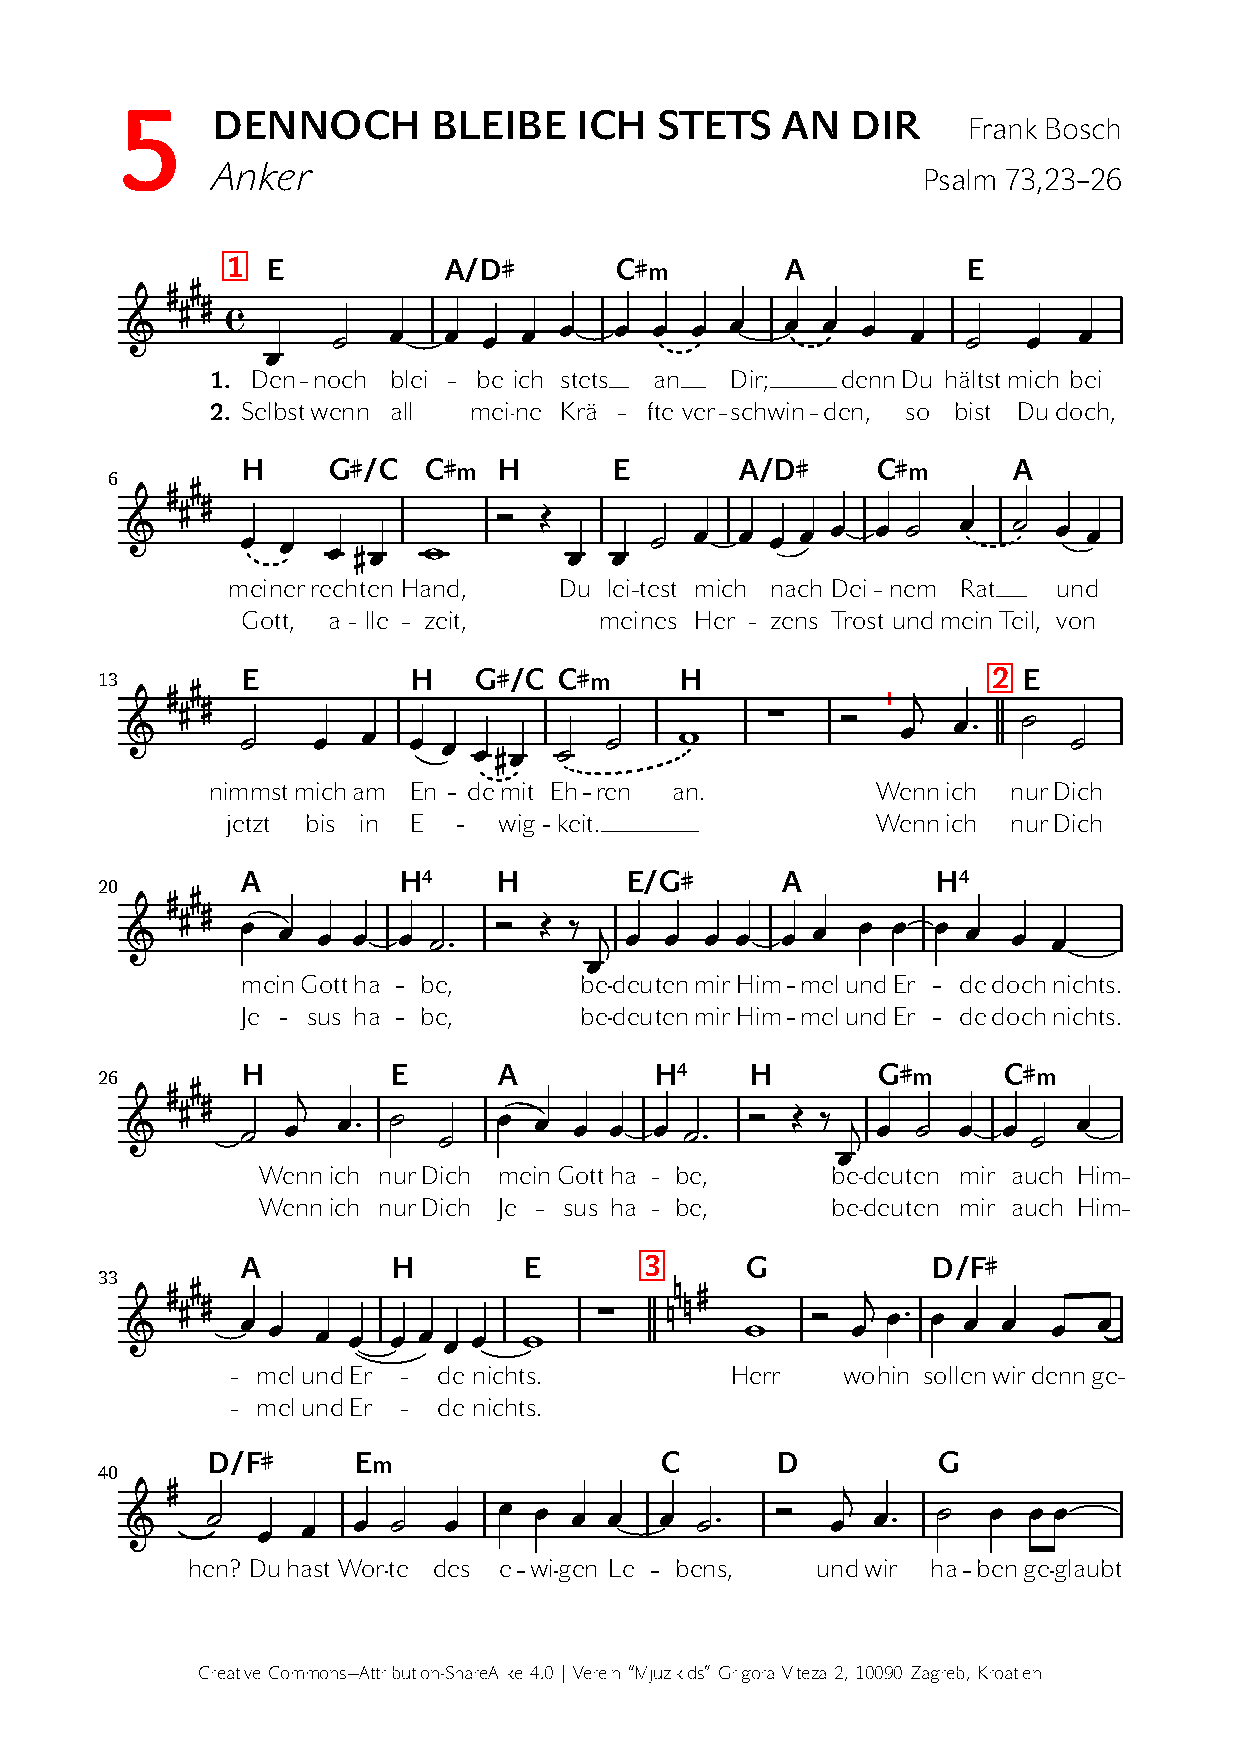
\includepdf[pages={1},noautoscale]{lilypond/de/src/05_wenn_ich_nur_dich_habe.pdf}
\end{minipage}

\newpage
\includepdf[pages={2},noautoscale,  %
    picturecommand={\setlength\unitlength{1cm}%
         \put(3.18,2.7){\includegraphics[width=0.86\linewidth,scale=1]{images/susanne/e5_wennichdichnurhabe}}}]%
         {lilypond/de/src/05_wenn_ich_nur_dich_habe.pdf}


%pjesma 6
\newpage
\phantomsection
\begin{minipage}[b]{0.5\linewidth}
\addcontentsline{toc}{section}{\texorpdfstring{{\rednifont\doccolor6.}\hspace{\onedigitspacing}}{}ANKER MEINE SEELE \ttfamily(Hebr 6,19)}
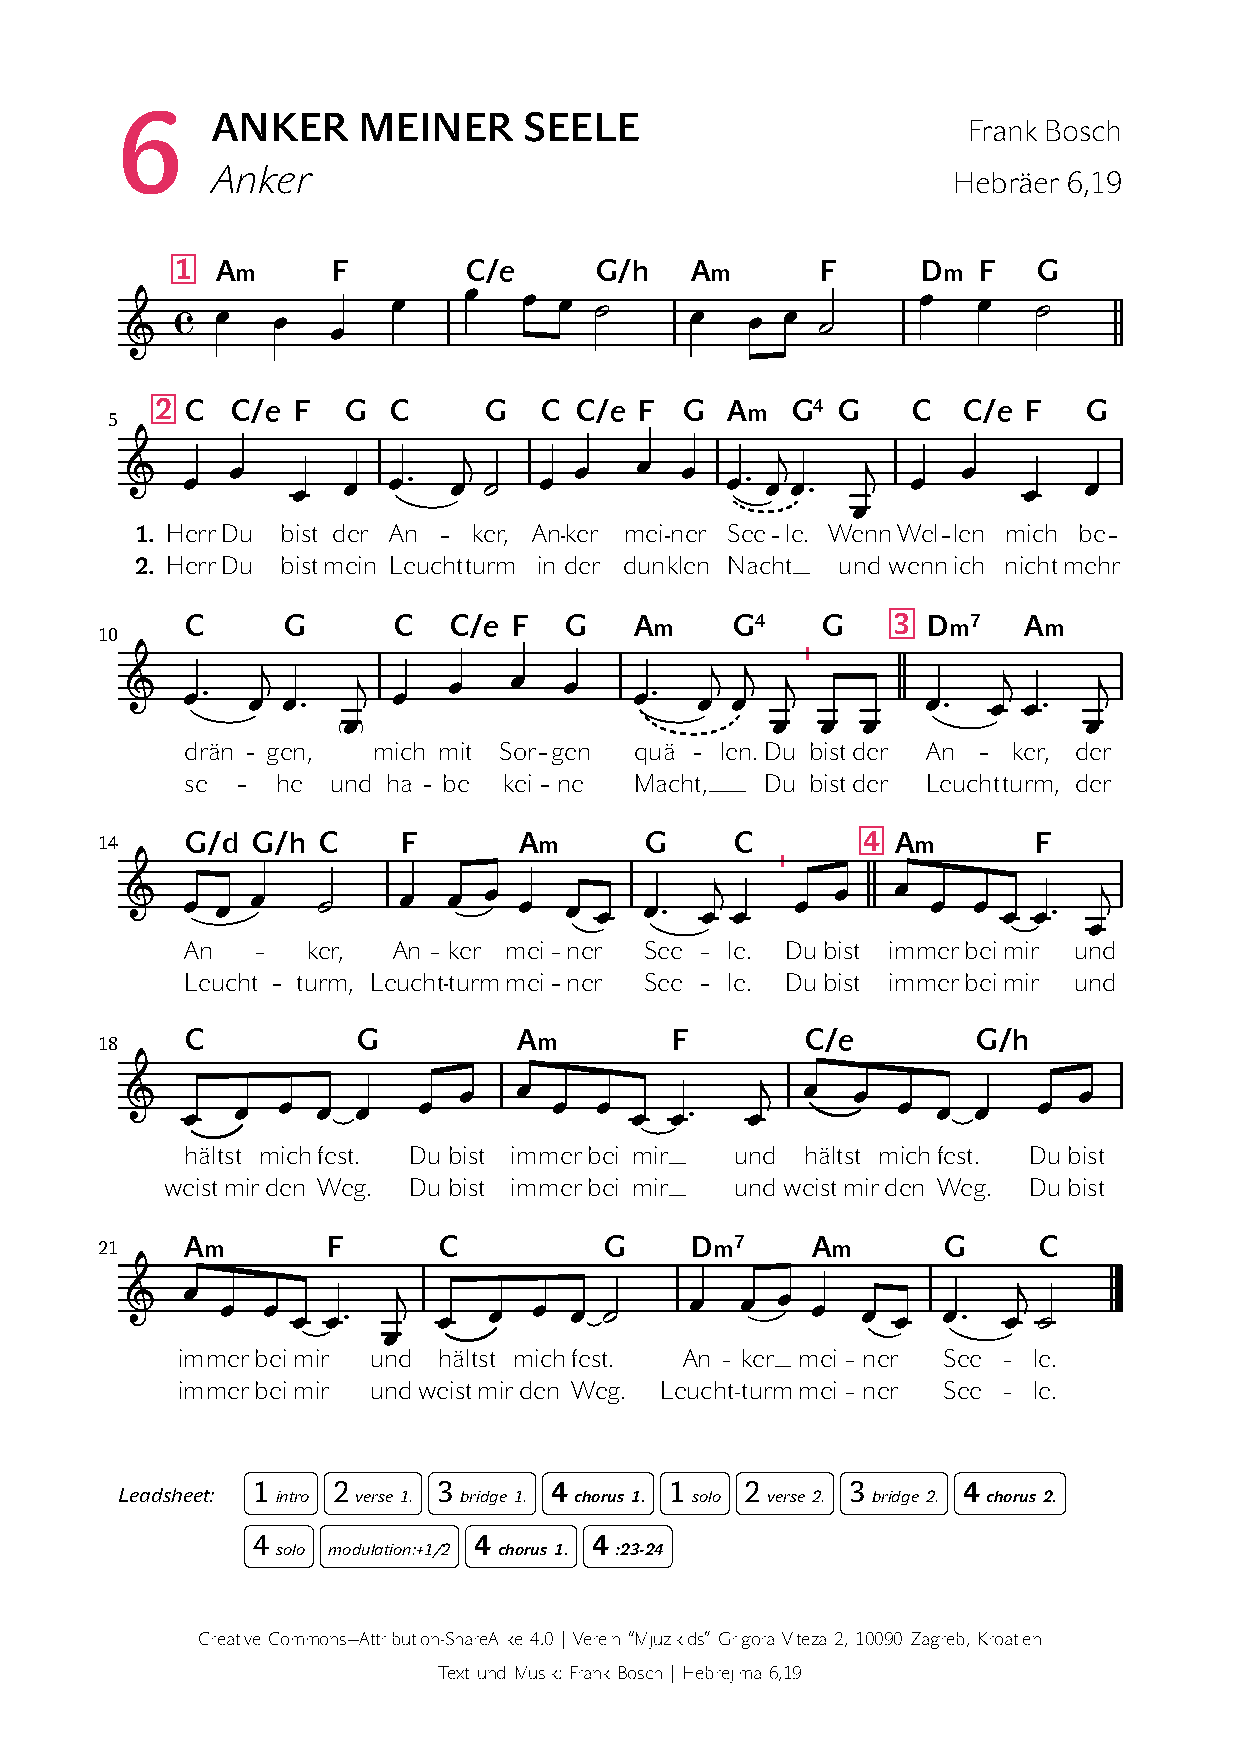
\includepdf[pages={1},noautoscale]{lilypond/de/src/06_anker_meine_seele.pdf}
\end{minipage}

\newpage
\begin{center}
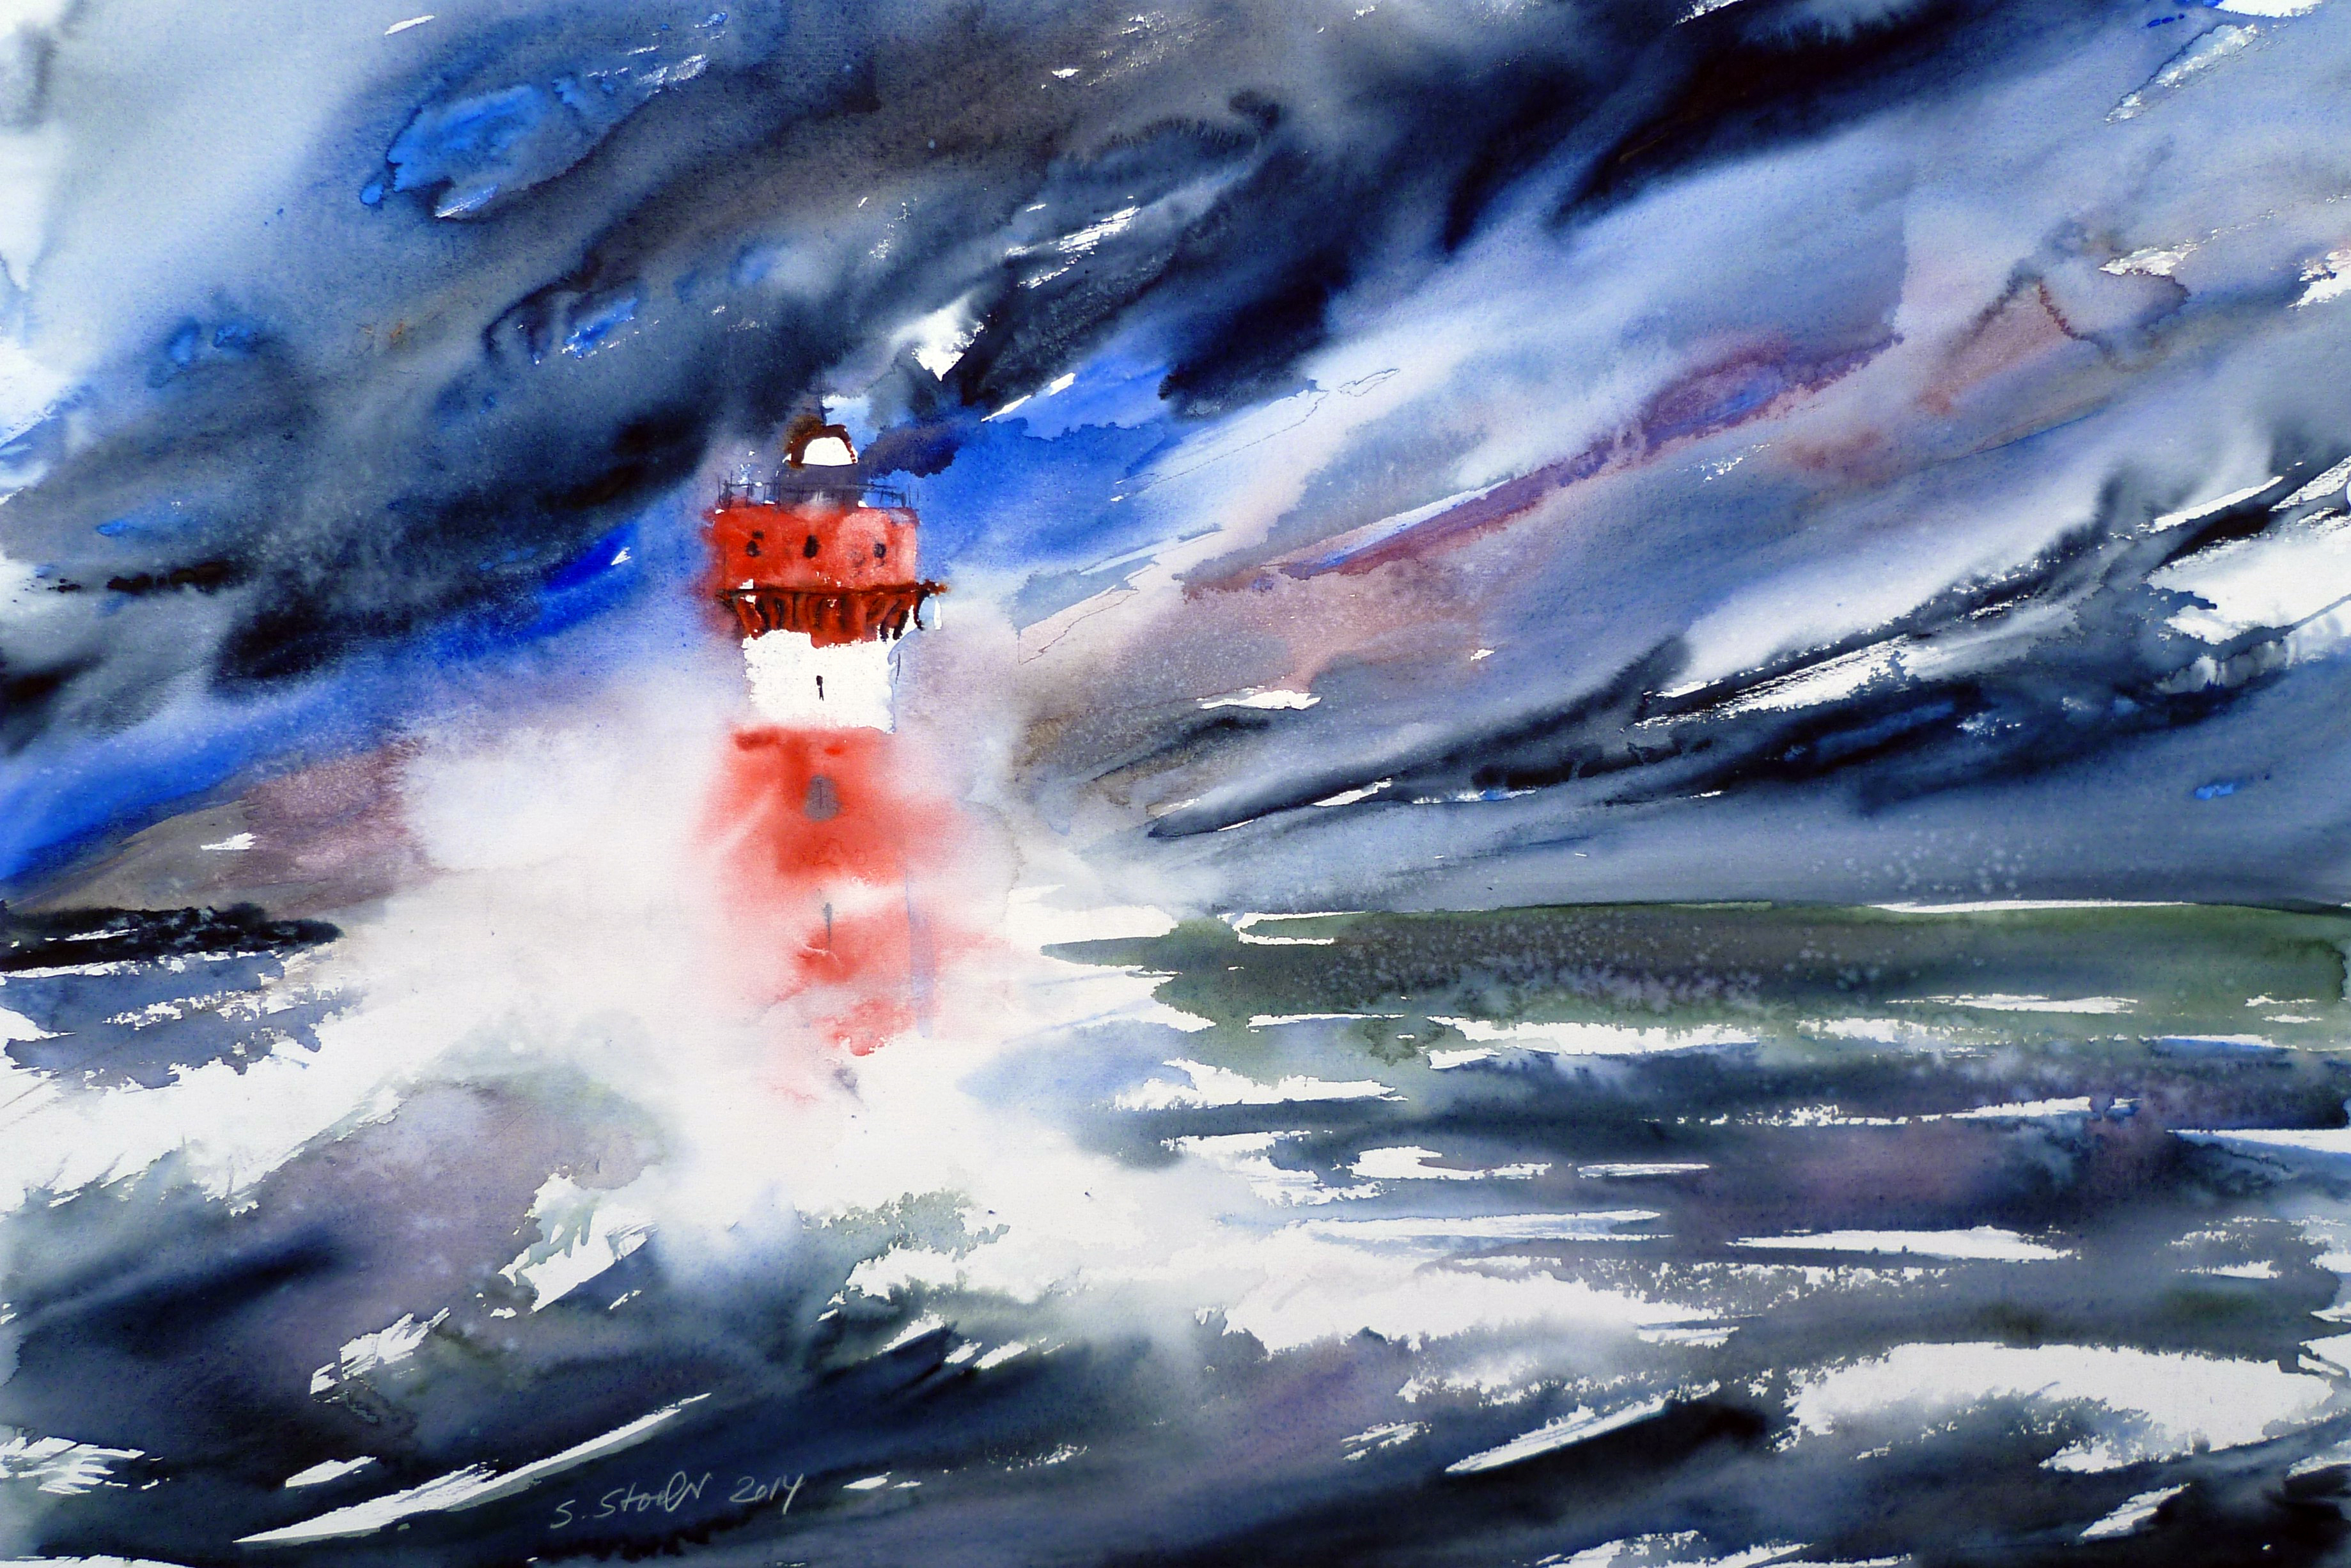
\includegraphics[width=\linewidth]{images/susanne/f6_ankermeinerseele}
\vfill
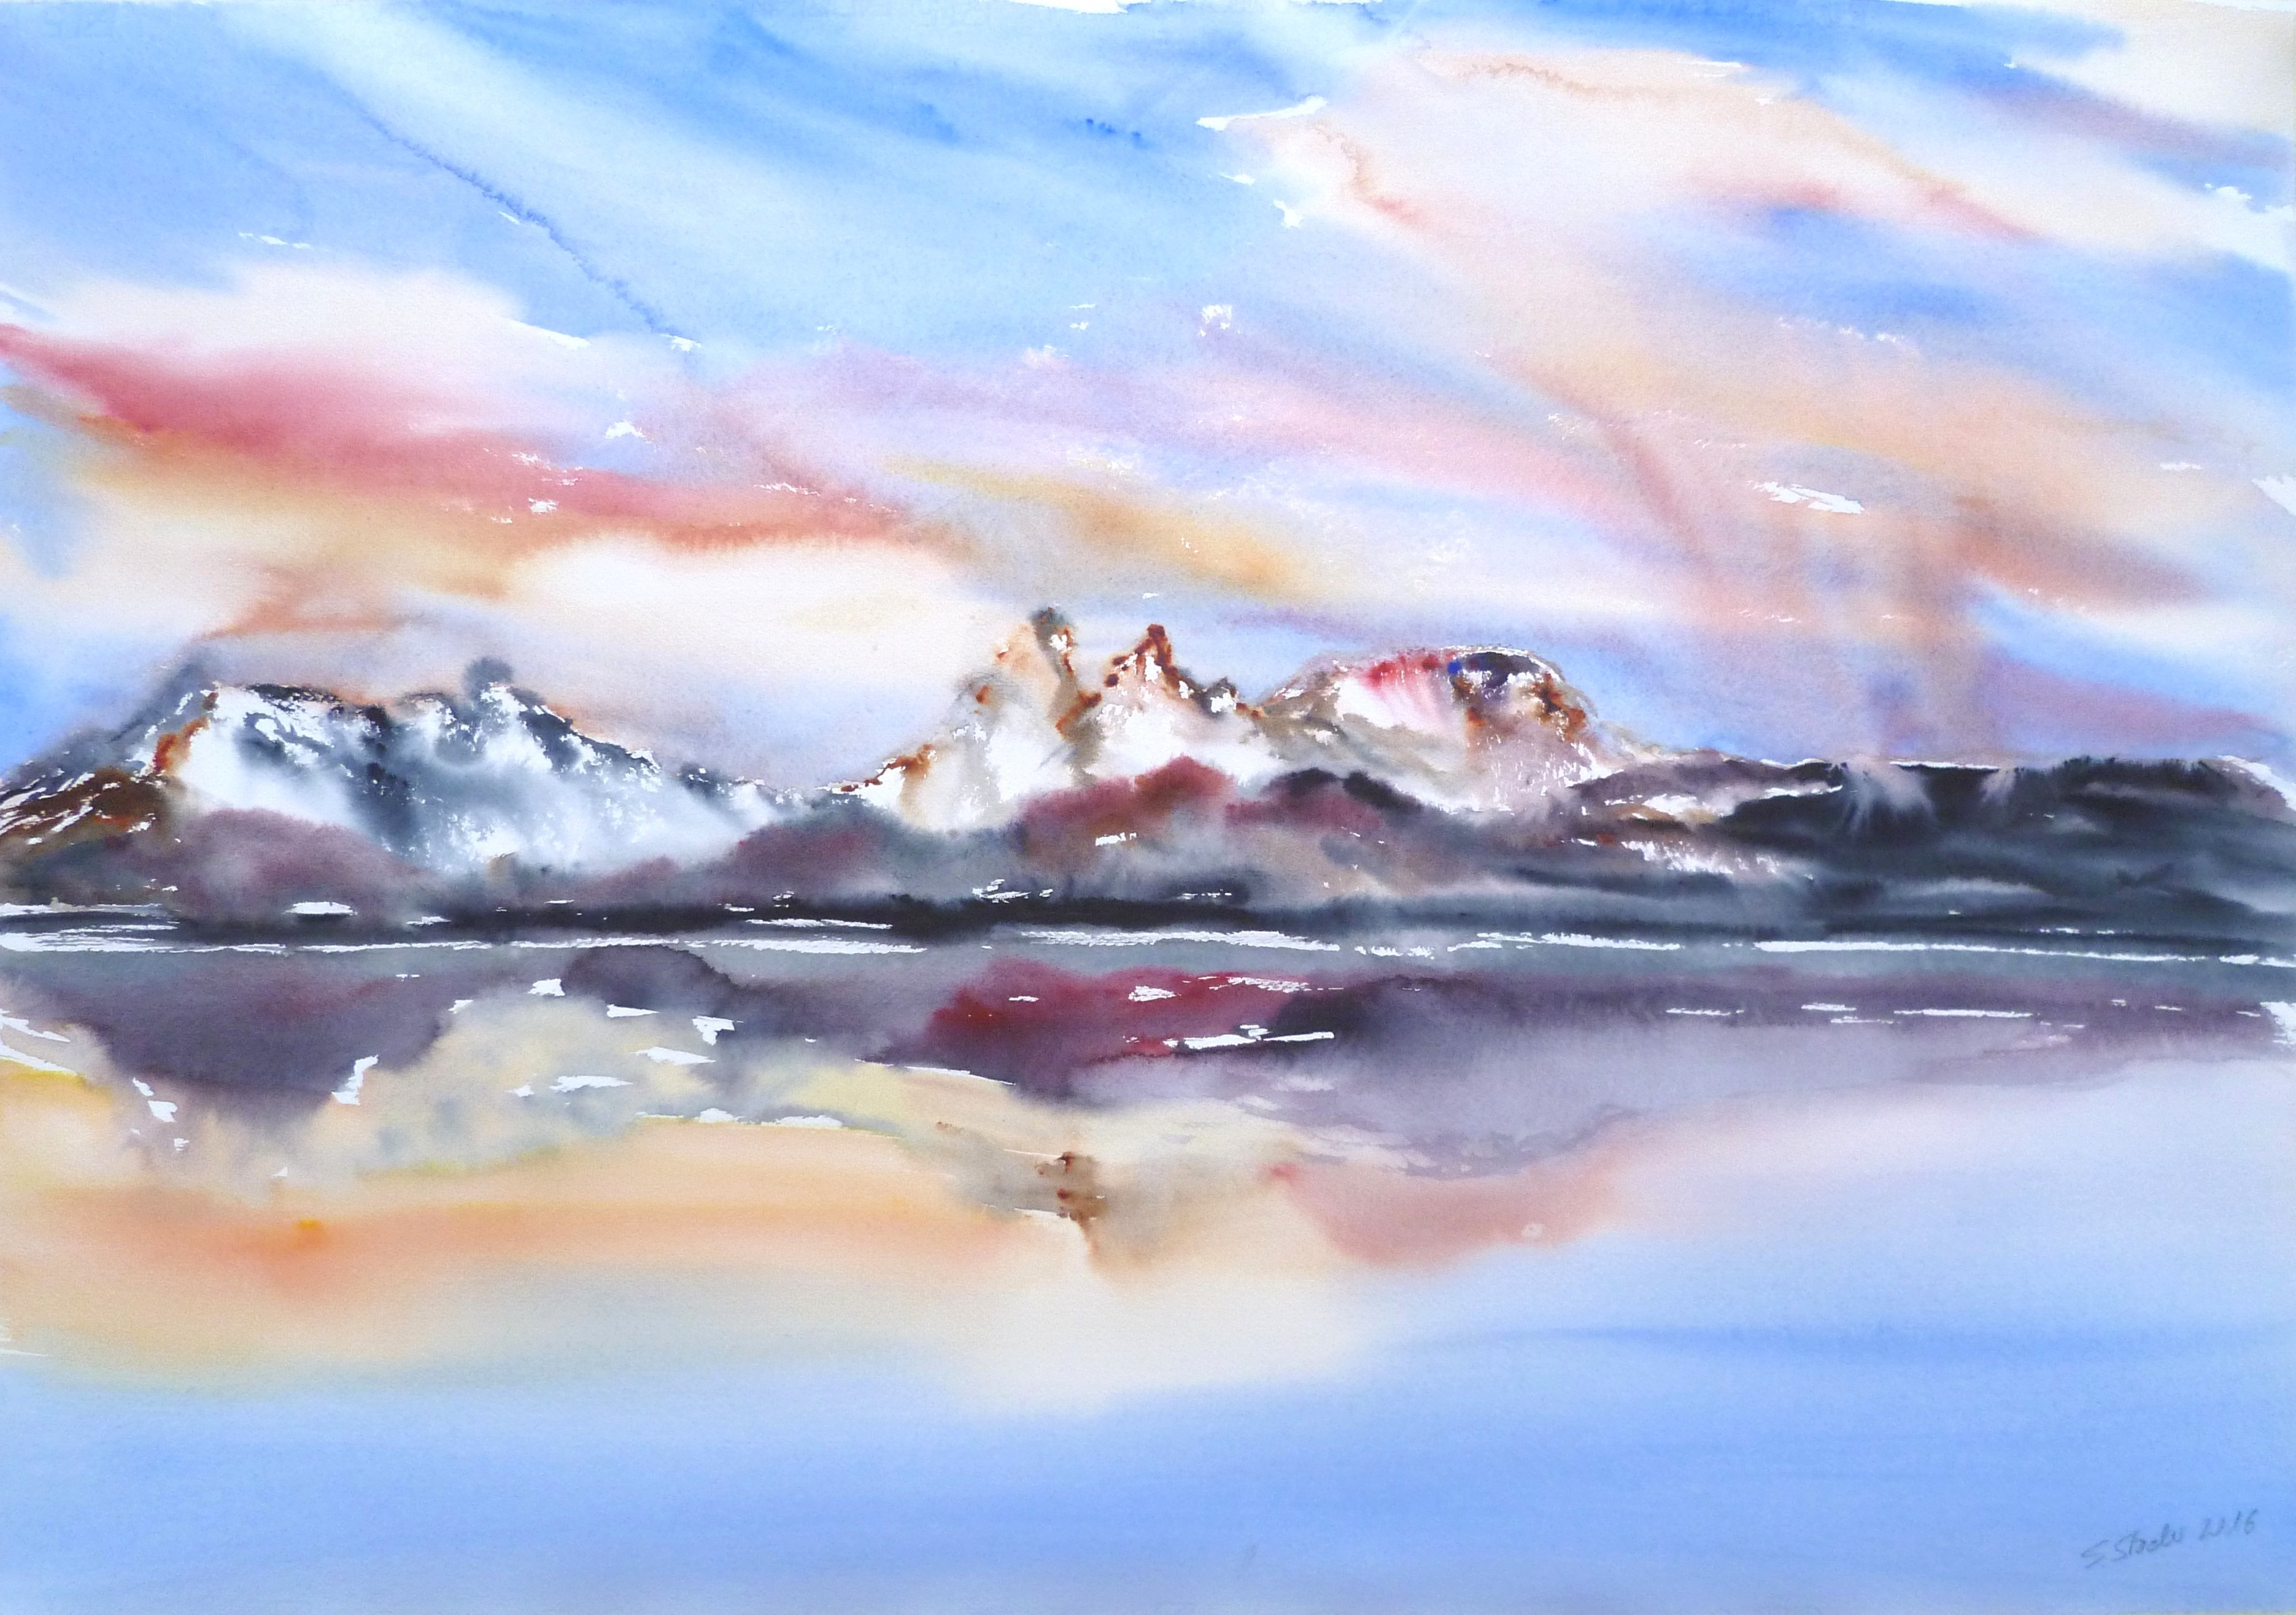
\includegraphics[width=\linewidth]{images/susanne/lagoconmontitramonto}
\end{center}

%pjesma 7
\newpage
\phantomsection
\begin{minipage}[b]{0.5\linewidth}
\addcontentsline{toc}{section}{\texorpdfstring{{\rednifont\doccolor7.}\hspace{\onedigitspacing}}{}NICHTS KANN UNS TRENNEN \ttfamily(Röm 8,35.37–39)}
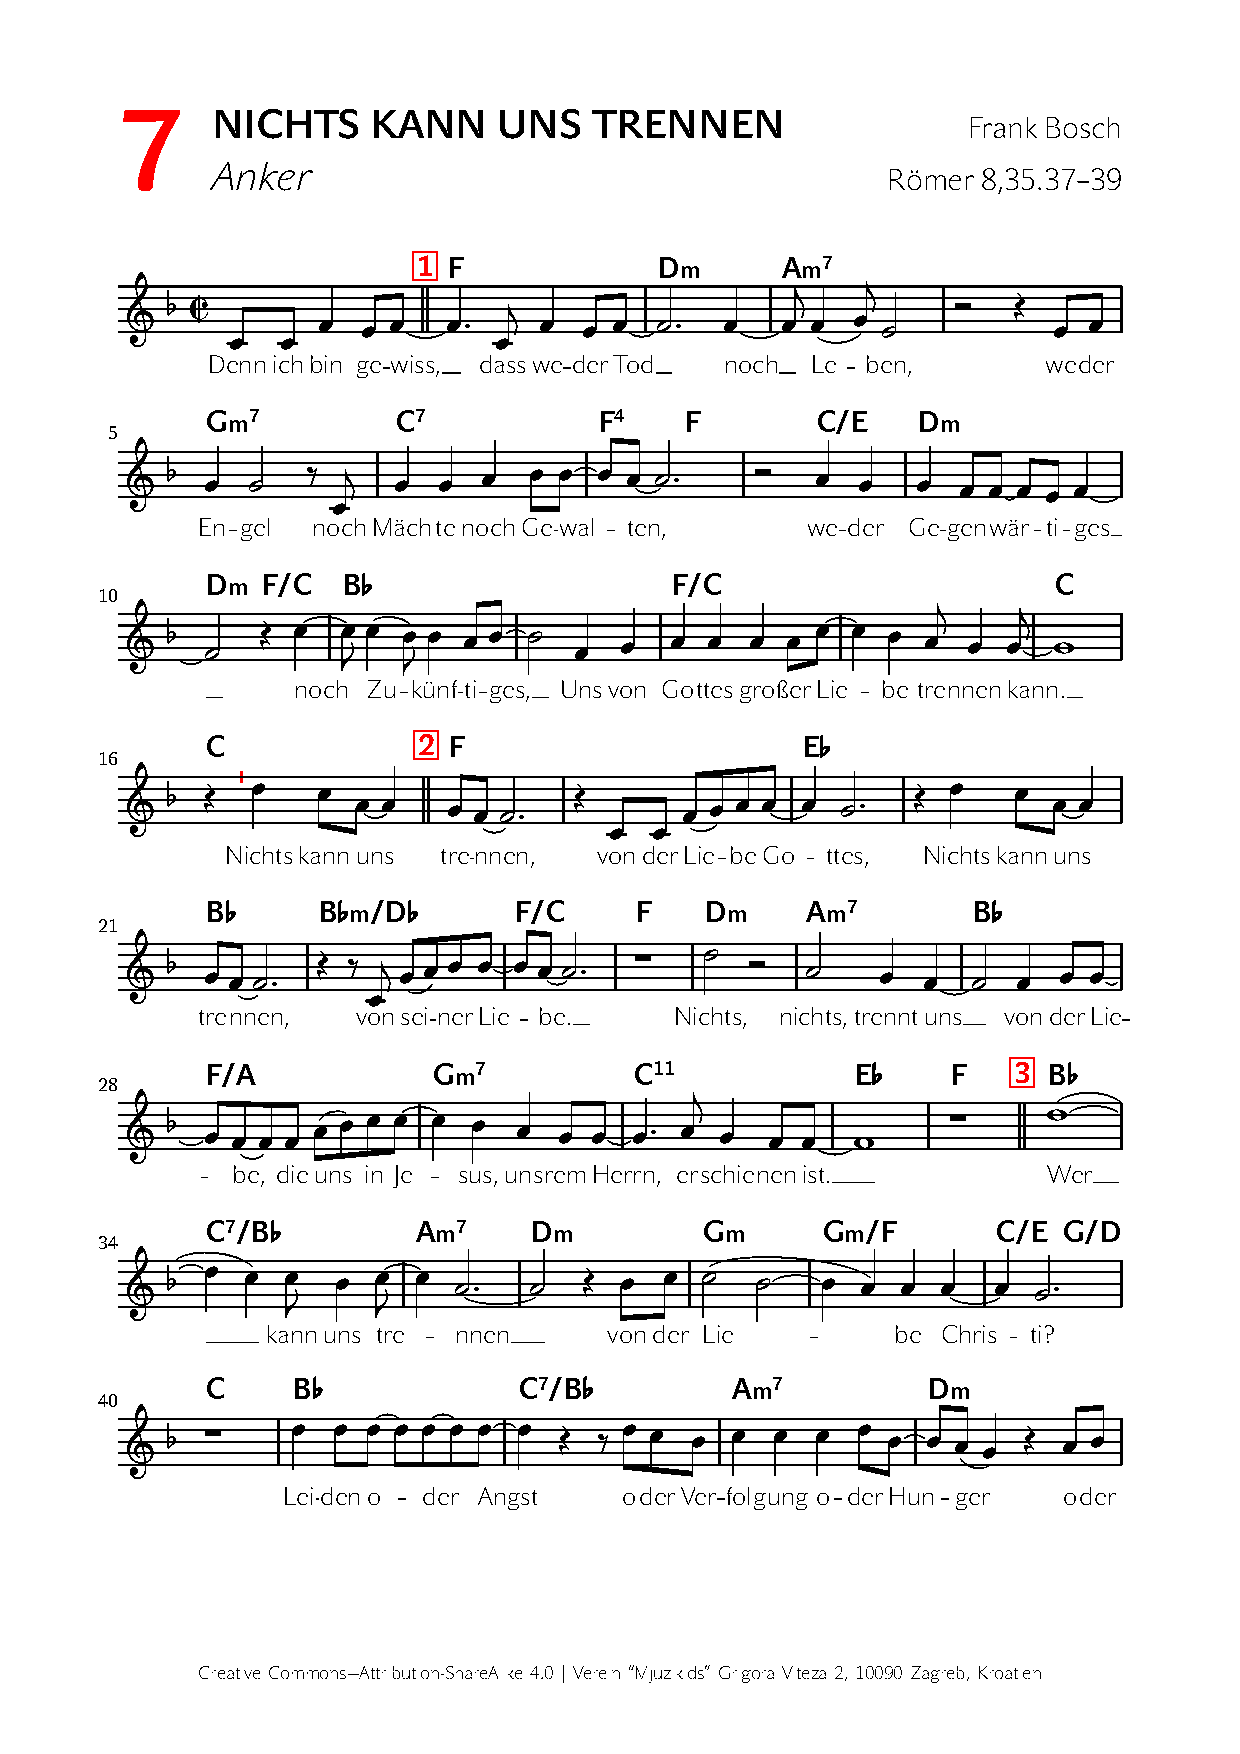
\includepdf[pages={1},noautoscale]{lilypond/de/src/07_nichts_kann_uns_trennen.pdf}
\end{minipage}

\newpage

\includepdf[pages={2},noautoscale,  %
    picturecommand={\setlength\unitlength{1cm}%
         \put(2,5){\includegraphics[width=\linewidth,scale=1]{images/susanne/g7_nichtskannunstrennen}}}]%
         {lilypond/de/src/07_nichts_kann_uns_trennen.pdf}


%pjesma 8
\newpage
\phantomsection
\begin{minipage}[b]{0.5\linewidth}
\addcontentsline{toc}{section}{\texorpdfstring{{\rednifont\doccolor8.}\hspace{\onedigitspacing}}{}ALLES AUF DEN KOPF GESTELLT \ttfamily(Mt 23,10–12)}
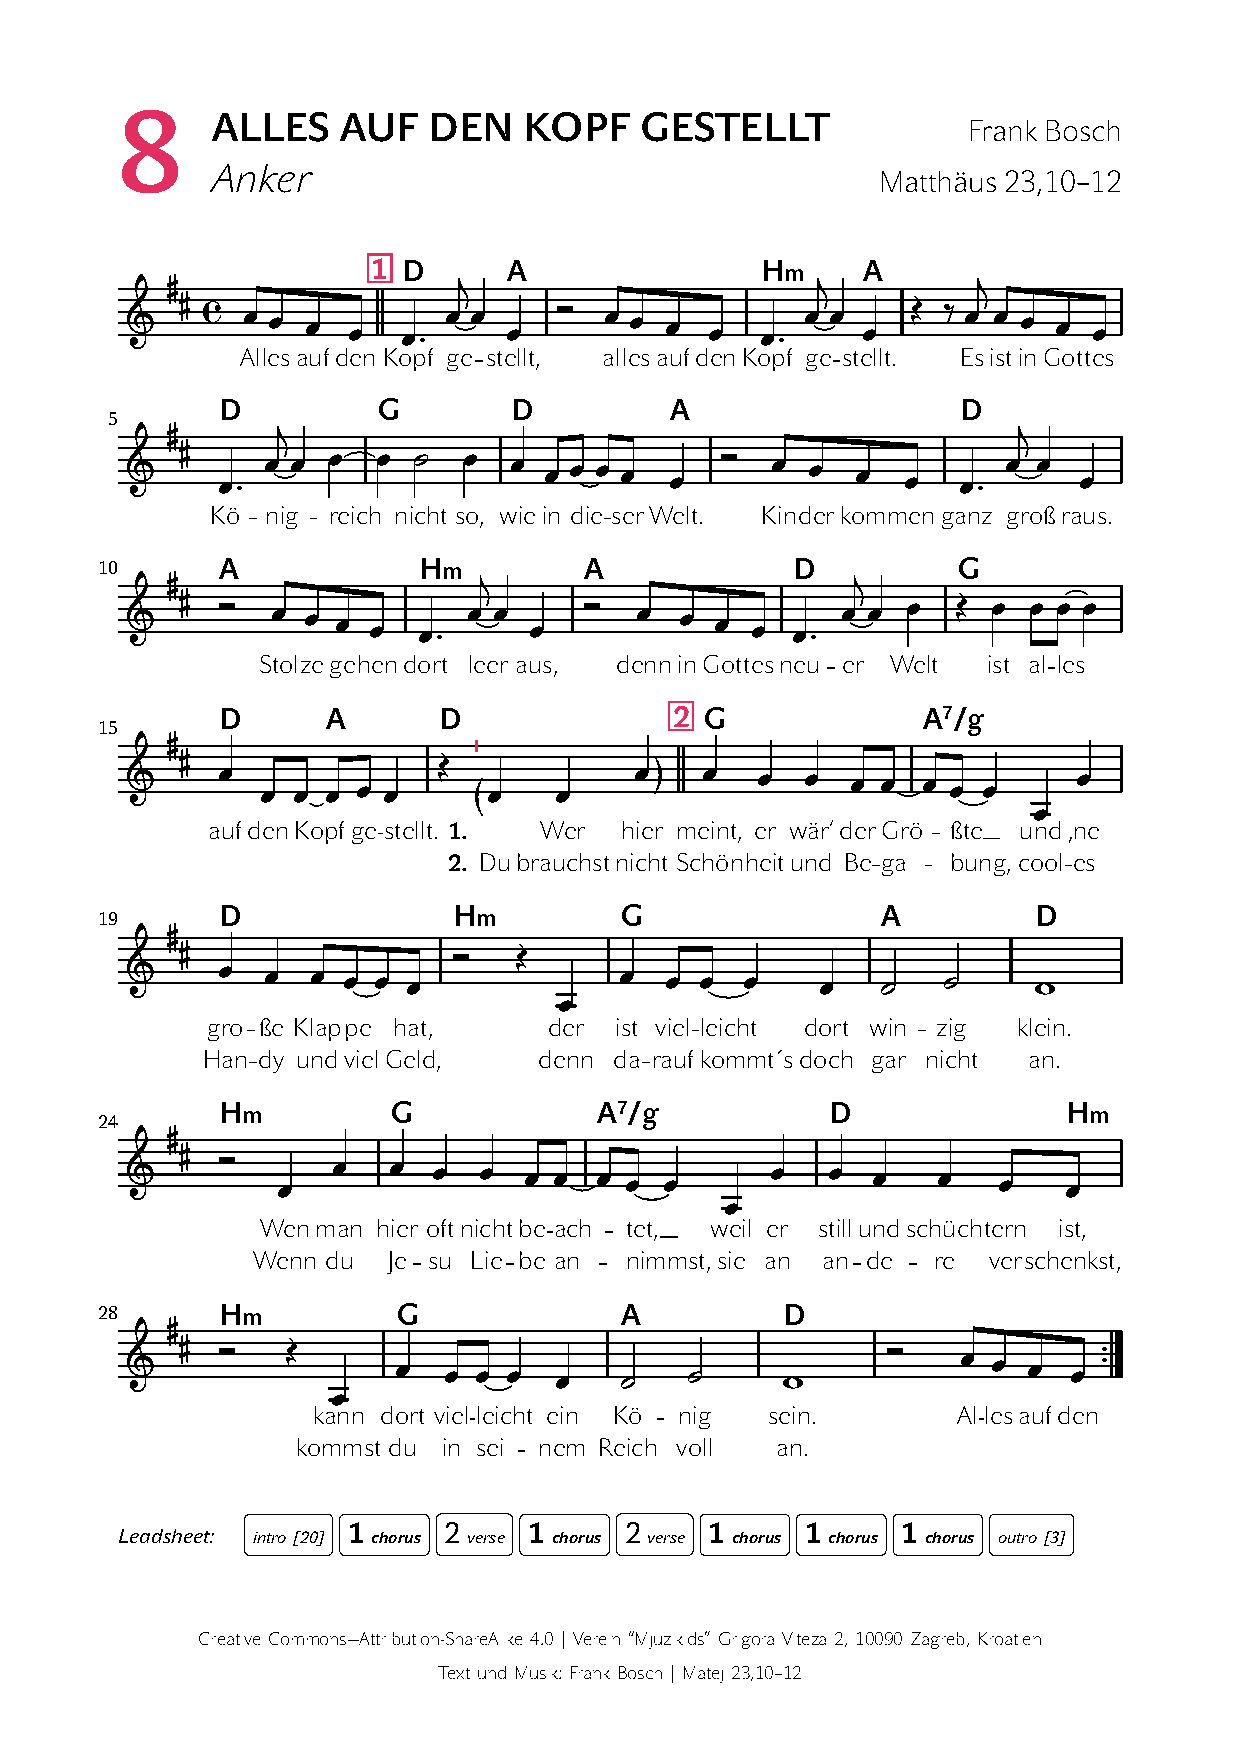
\includepdf[pages={1},noautoscale]{lilypond/de/src/08_alles_auf_den_kopf_gestellt.pdf}
\end{minipage}

\newpage
\begin{center}
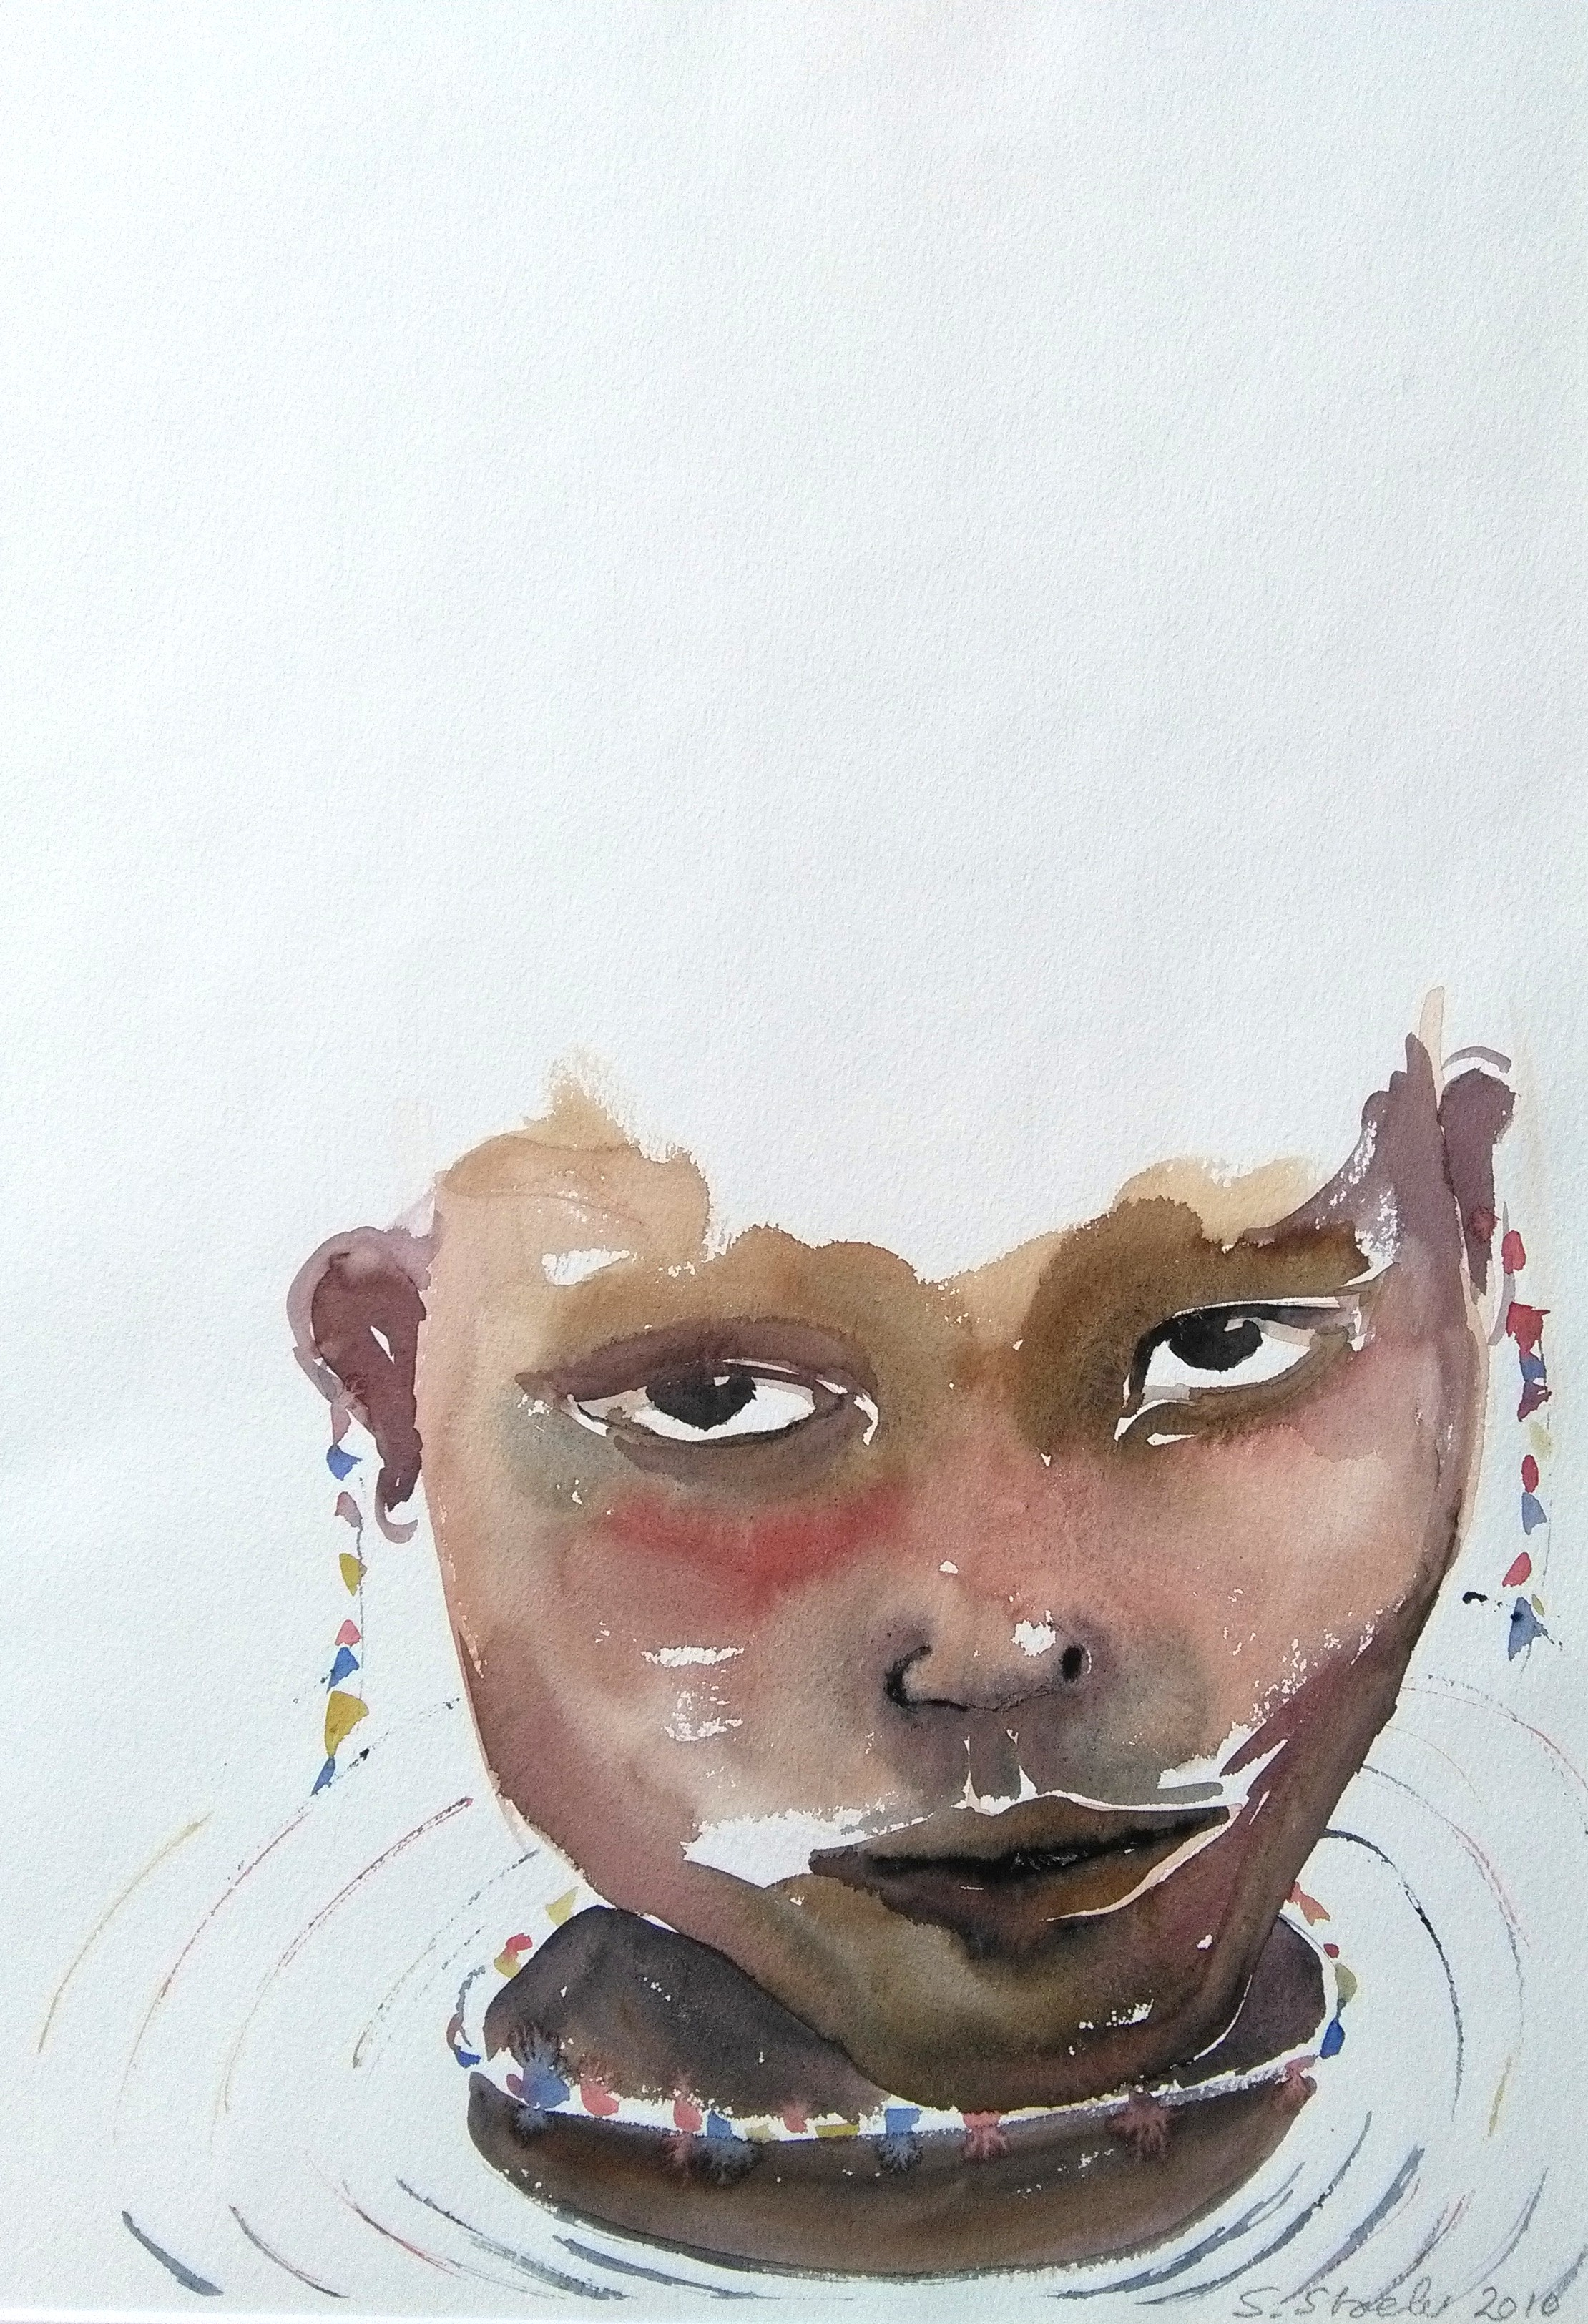
\includegraphics[width=0.95\linewidth]{images/susanne/h8_allesaufdenkopfgestellt}
\end{center}

%pjesme za djeca spava
\addtocontents{toc}{\cftpagenumbersoff{section}}
\addcontentsline{toc}{section}{\texorpdfstring{\ttfamily\hspace{7.7mm}}{}KINDERECKE}
\addtocontents{toc}{\cftpagenumberson{section}} % to restore the showing of page numbers

%pjesma 9
\newpage
\phantomsection
\begin{minipage}[b]{0.5\linewidth}
\addcontentsline{toc}{section}{\texorpdfstring{{\rednifont\doccolor9.}\hspace{\onedigitspacing}}{}SUPER PAPA \ttfamily(Röm 8,15)}
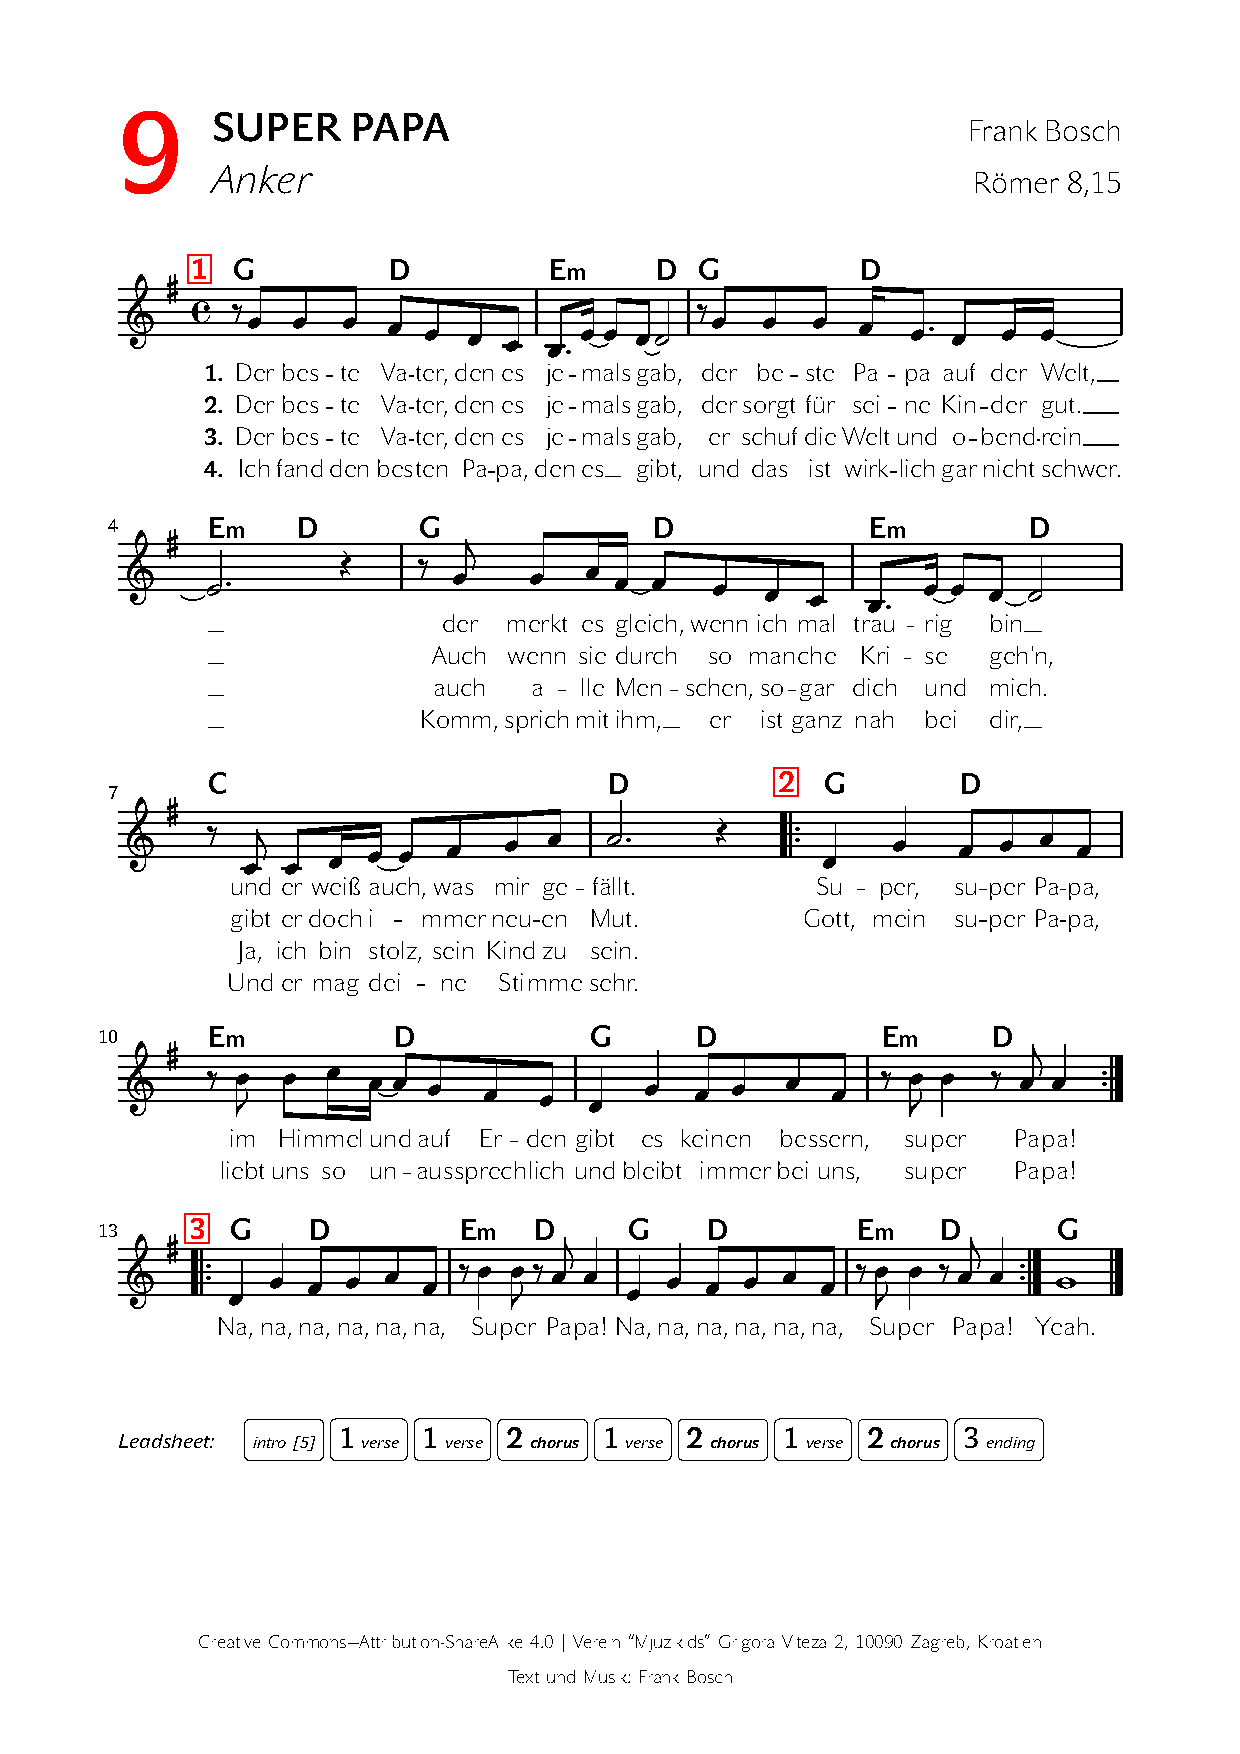
\includepdf[pages={1},noautoscale]{lilypond/de/src/09_super_papa.pdf}
\end{minipage}

\newpage
\begin{center}
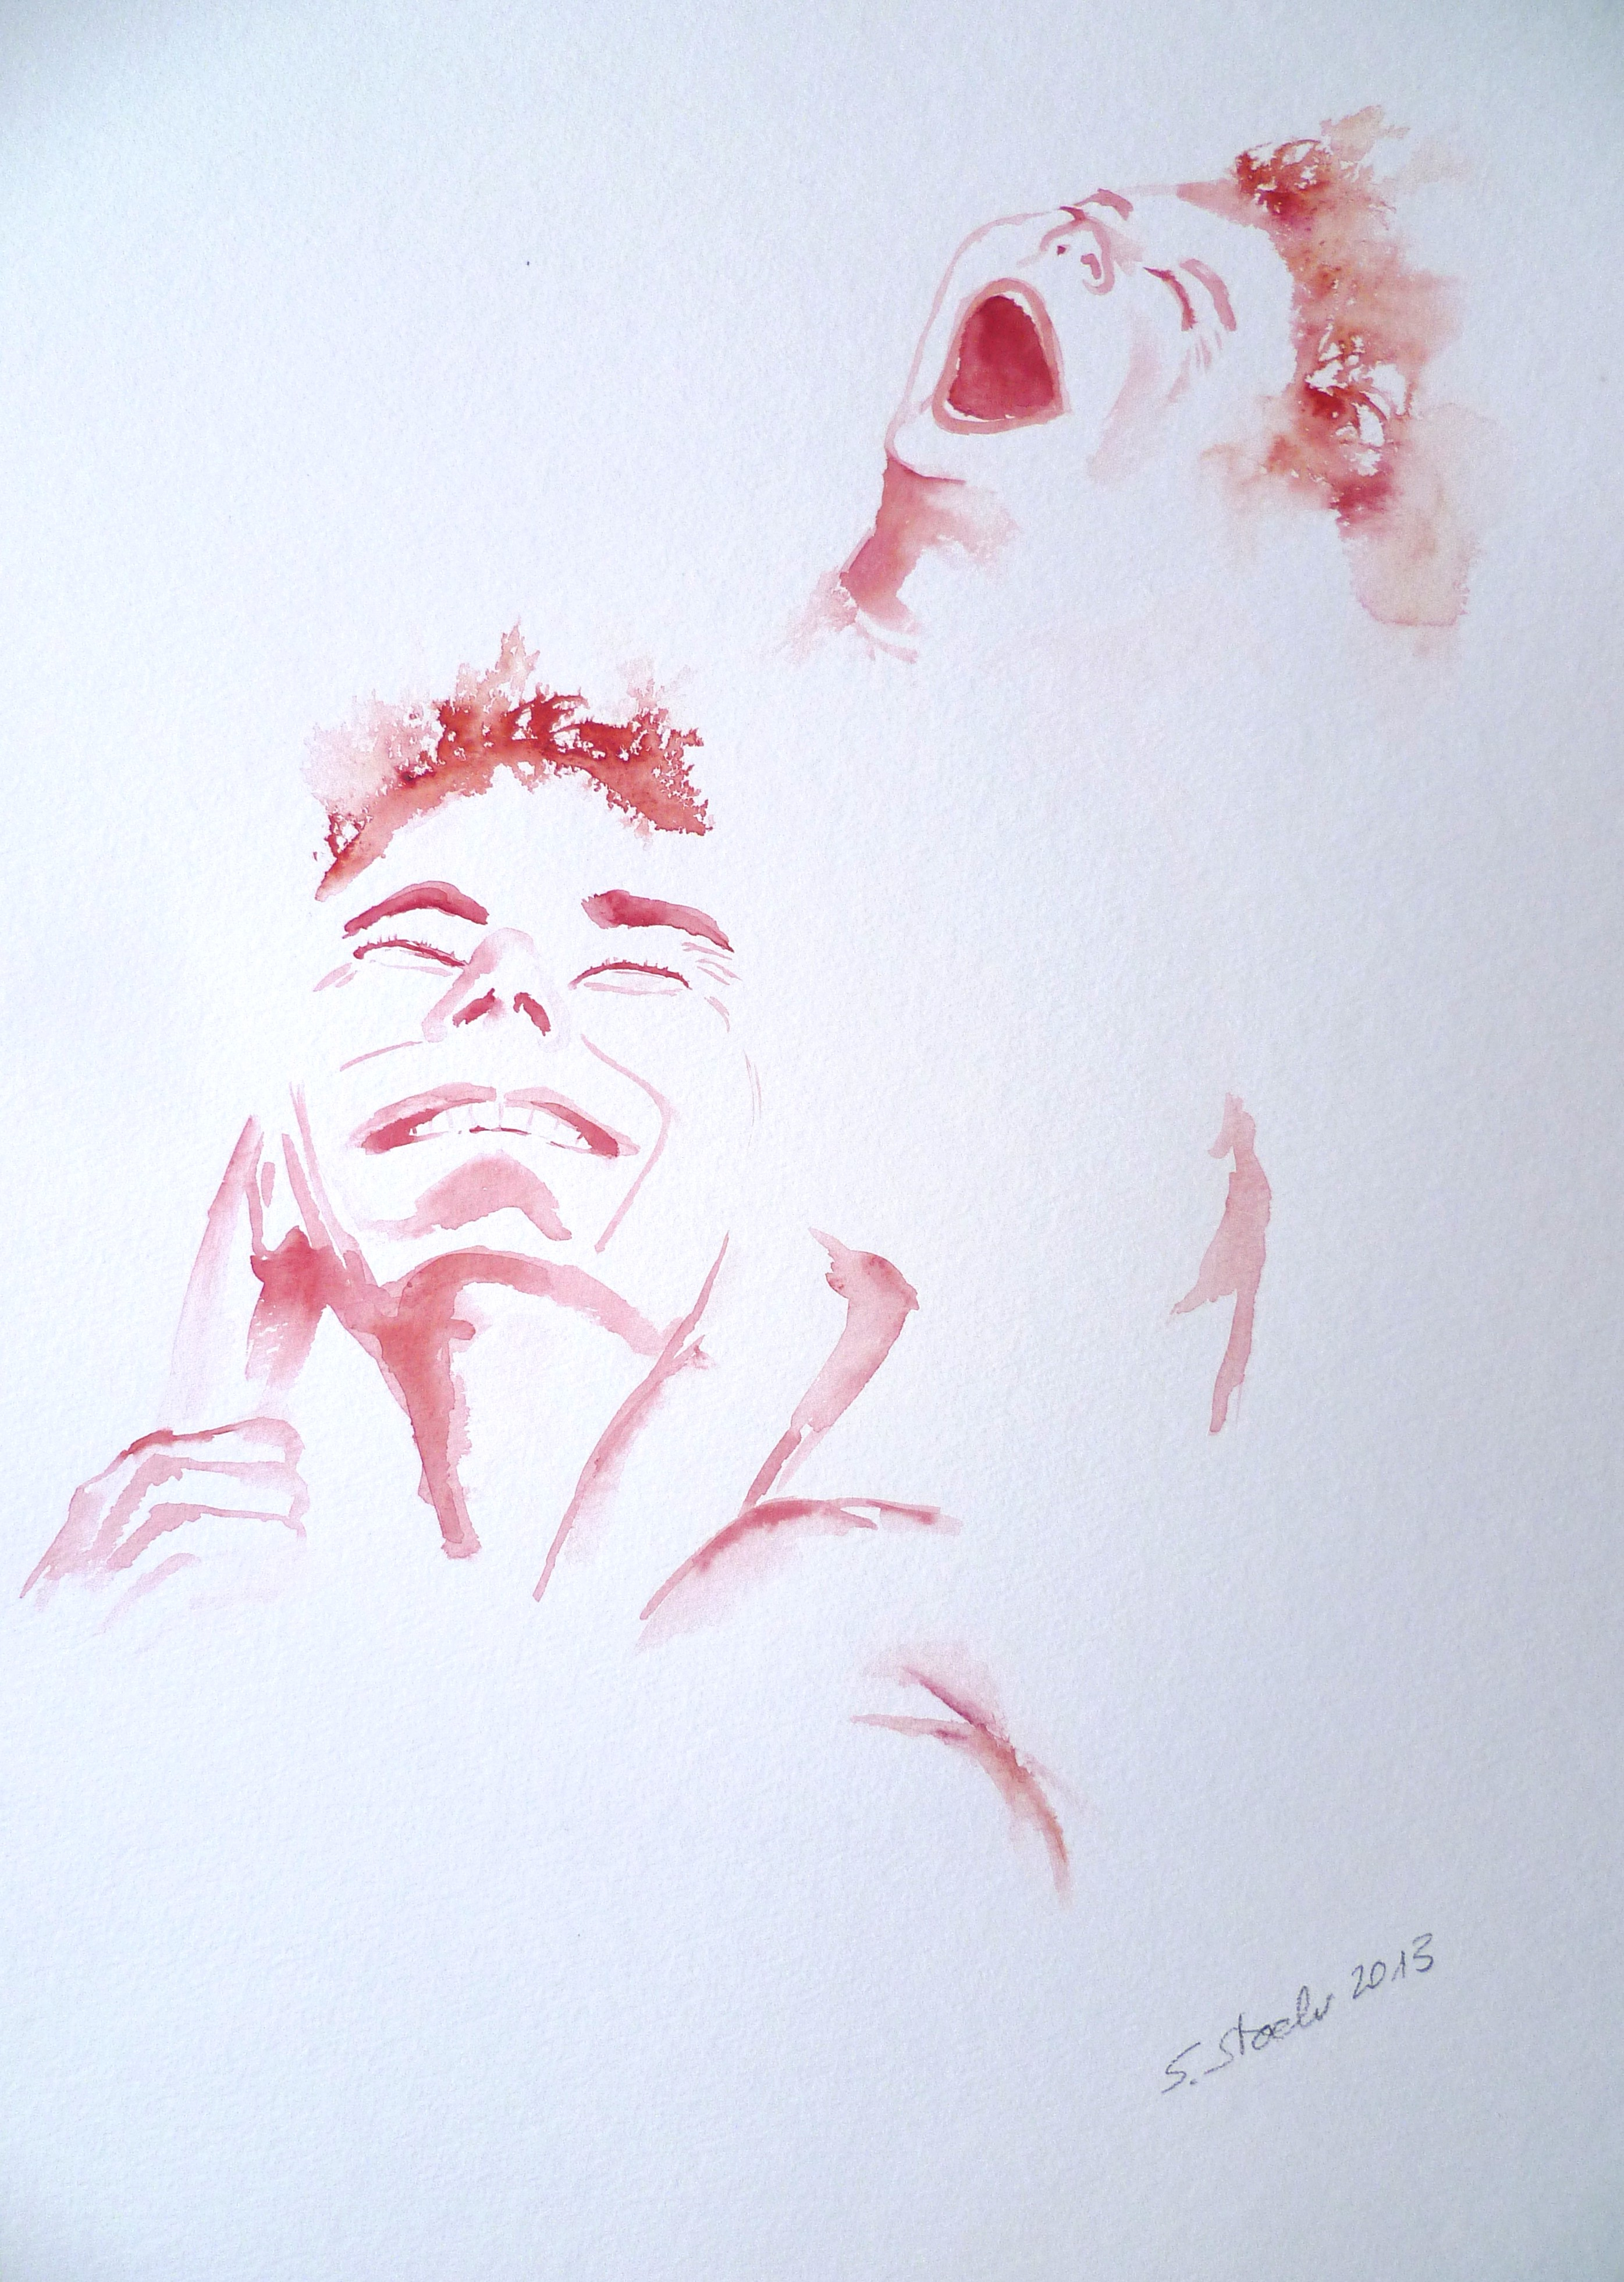
\includegraphics[width=\linewidth]{images/susanne/i9_superpapa}
\end{center}

%pjesma 10
\newpage
\phantomsection
\begin{minipage}[b]{0.5\linewidth}
\addcontentsline{toc}{section}{\texorpdfstring{{\rednifont\doccolor10.}\hspace{\twodigitspacing}}{}EIN HAUPTGEWINN \ttfamily(Ps 139,14)}
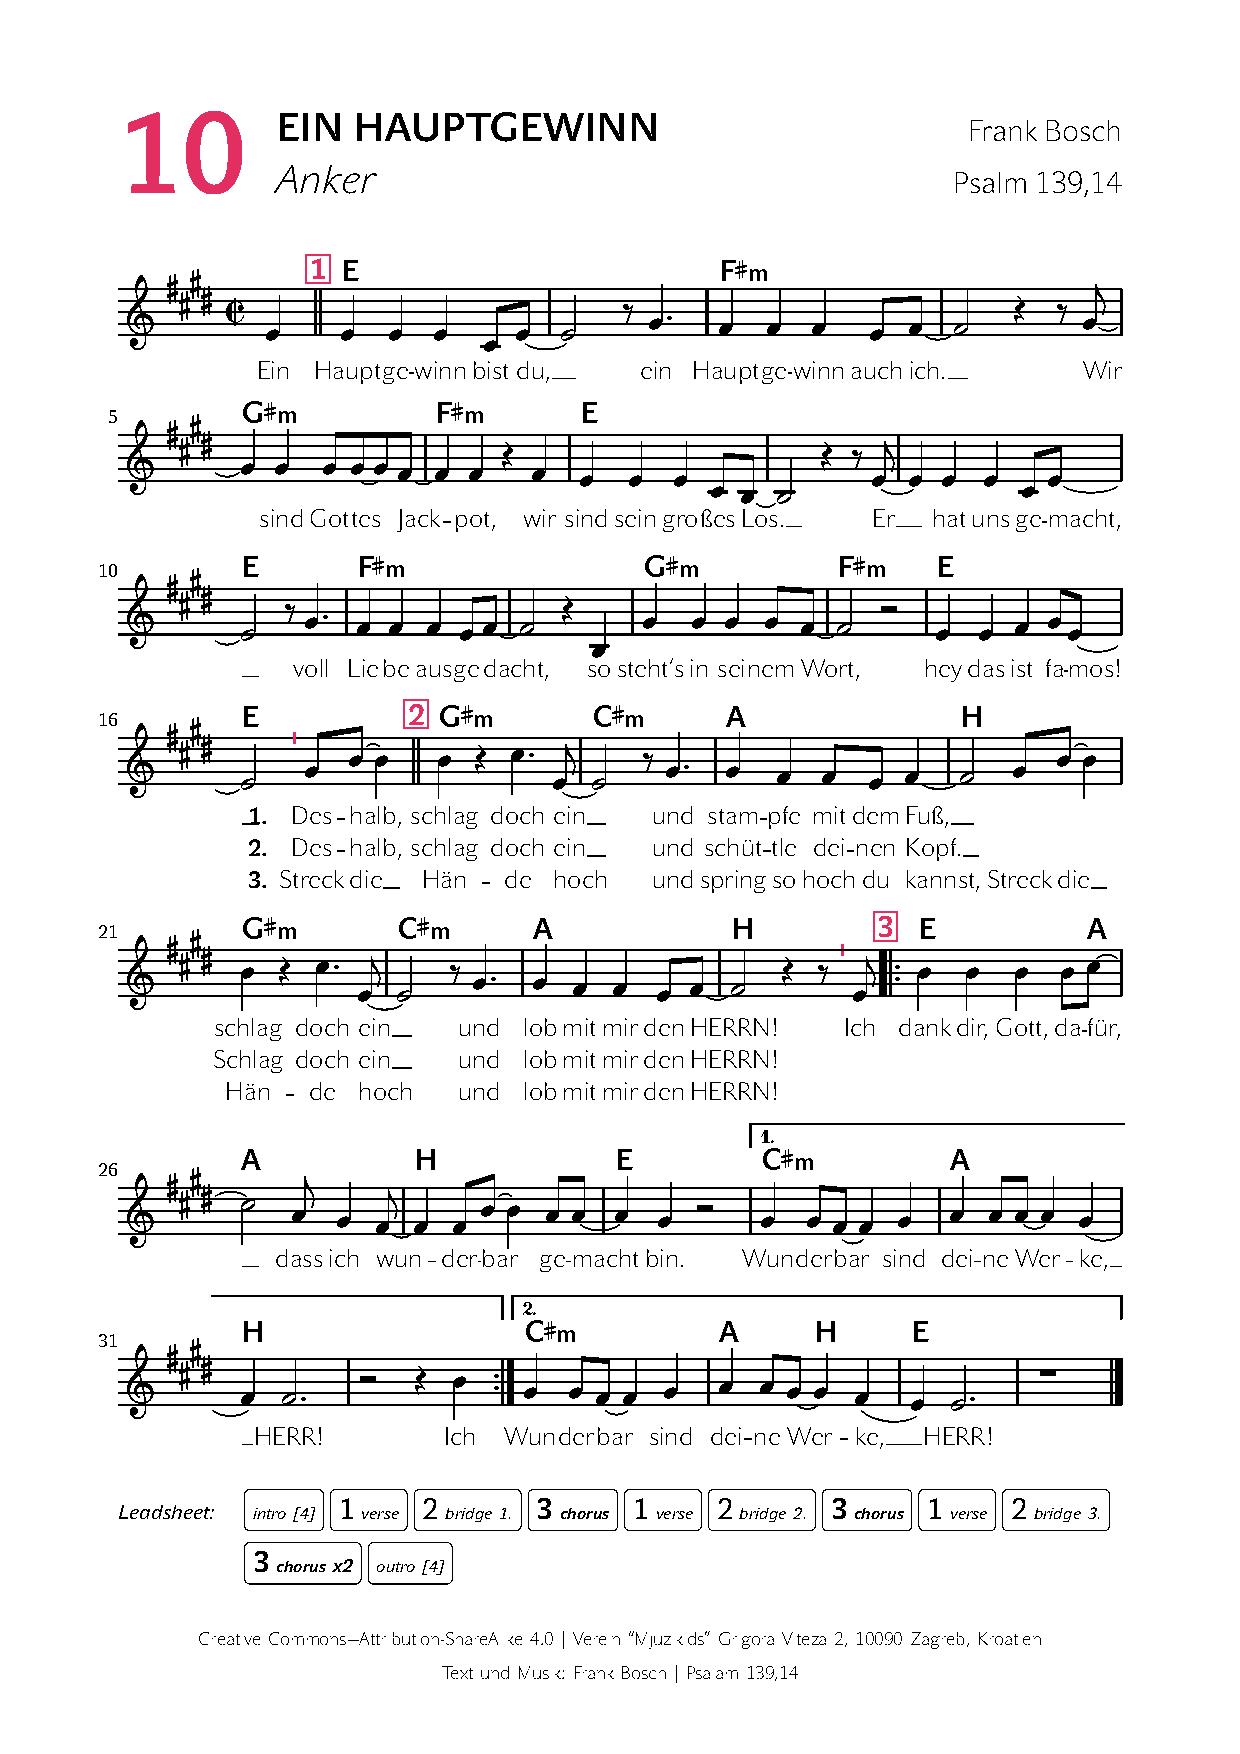
\includepdf[pages={1},noautoscale]{lilypond/de/src/10_ein_hauptgewinn.pdf}
\end{minipage}

\newpage
\begin{center}
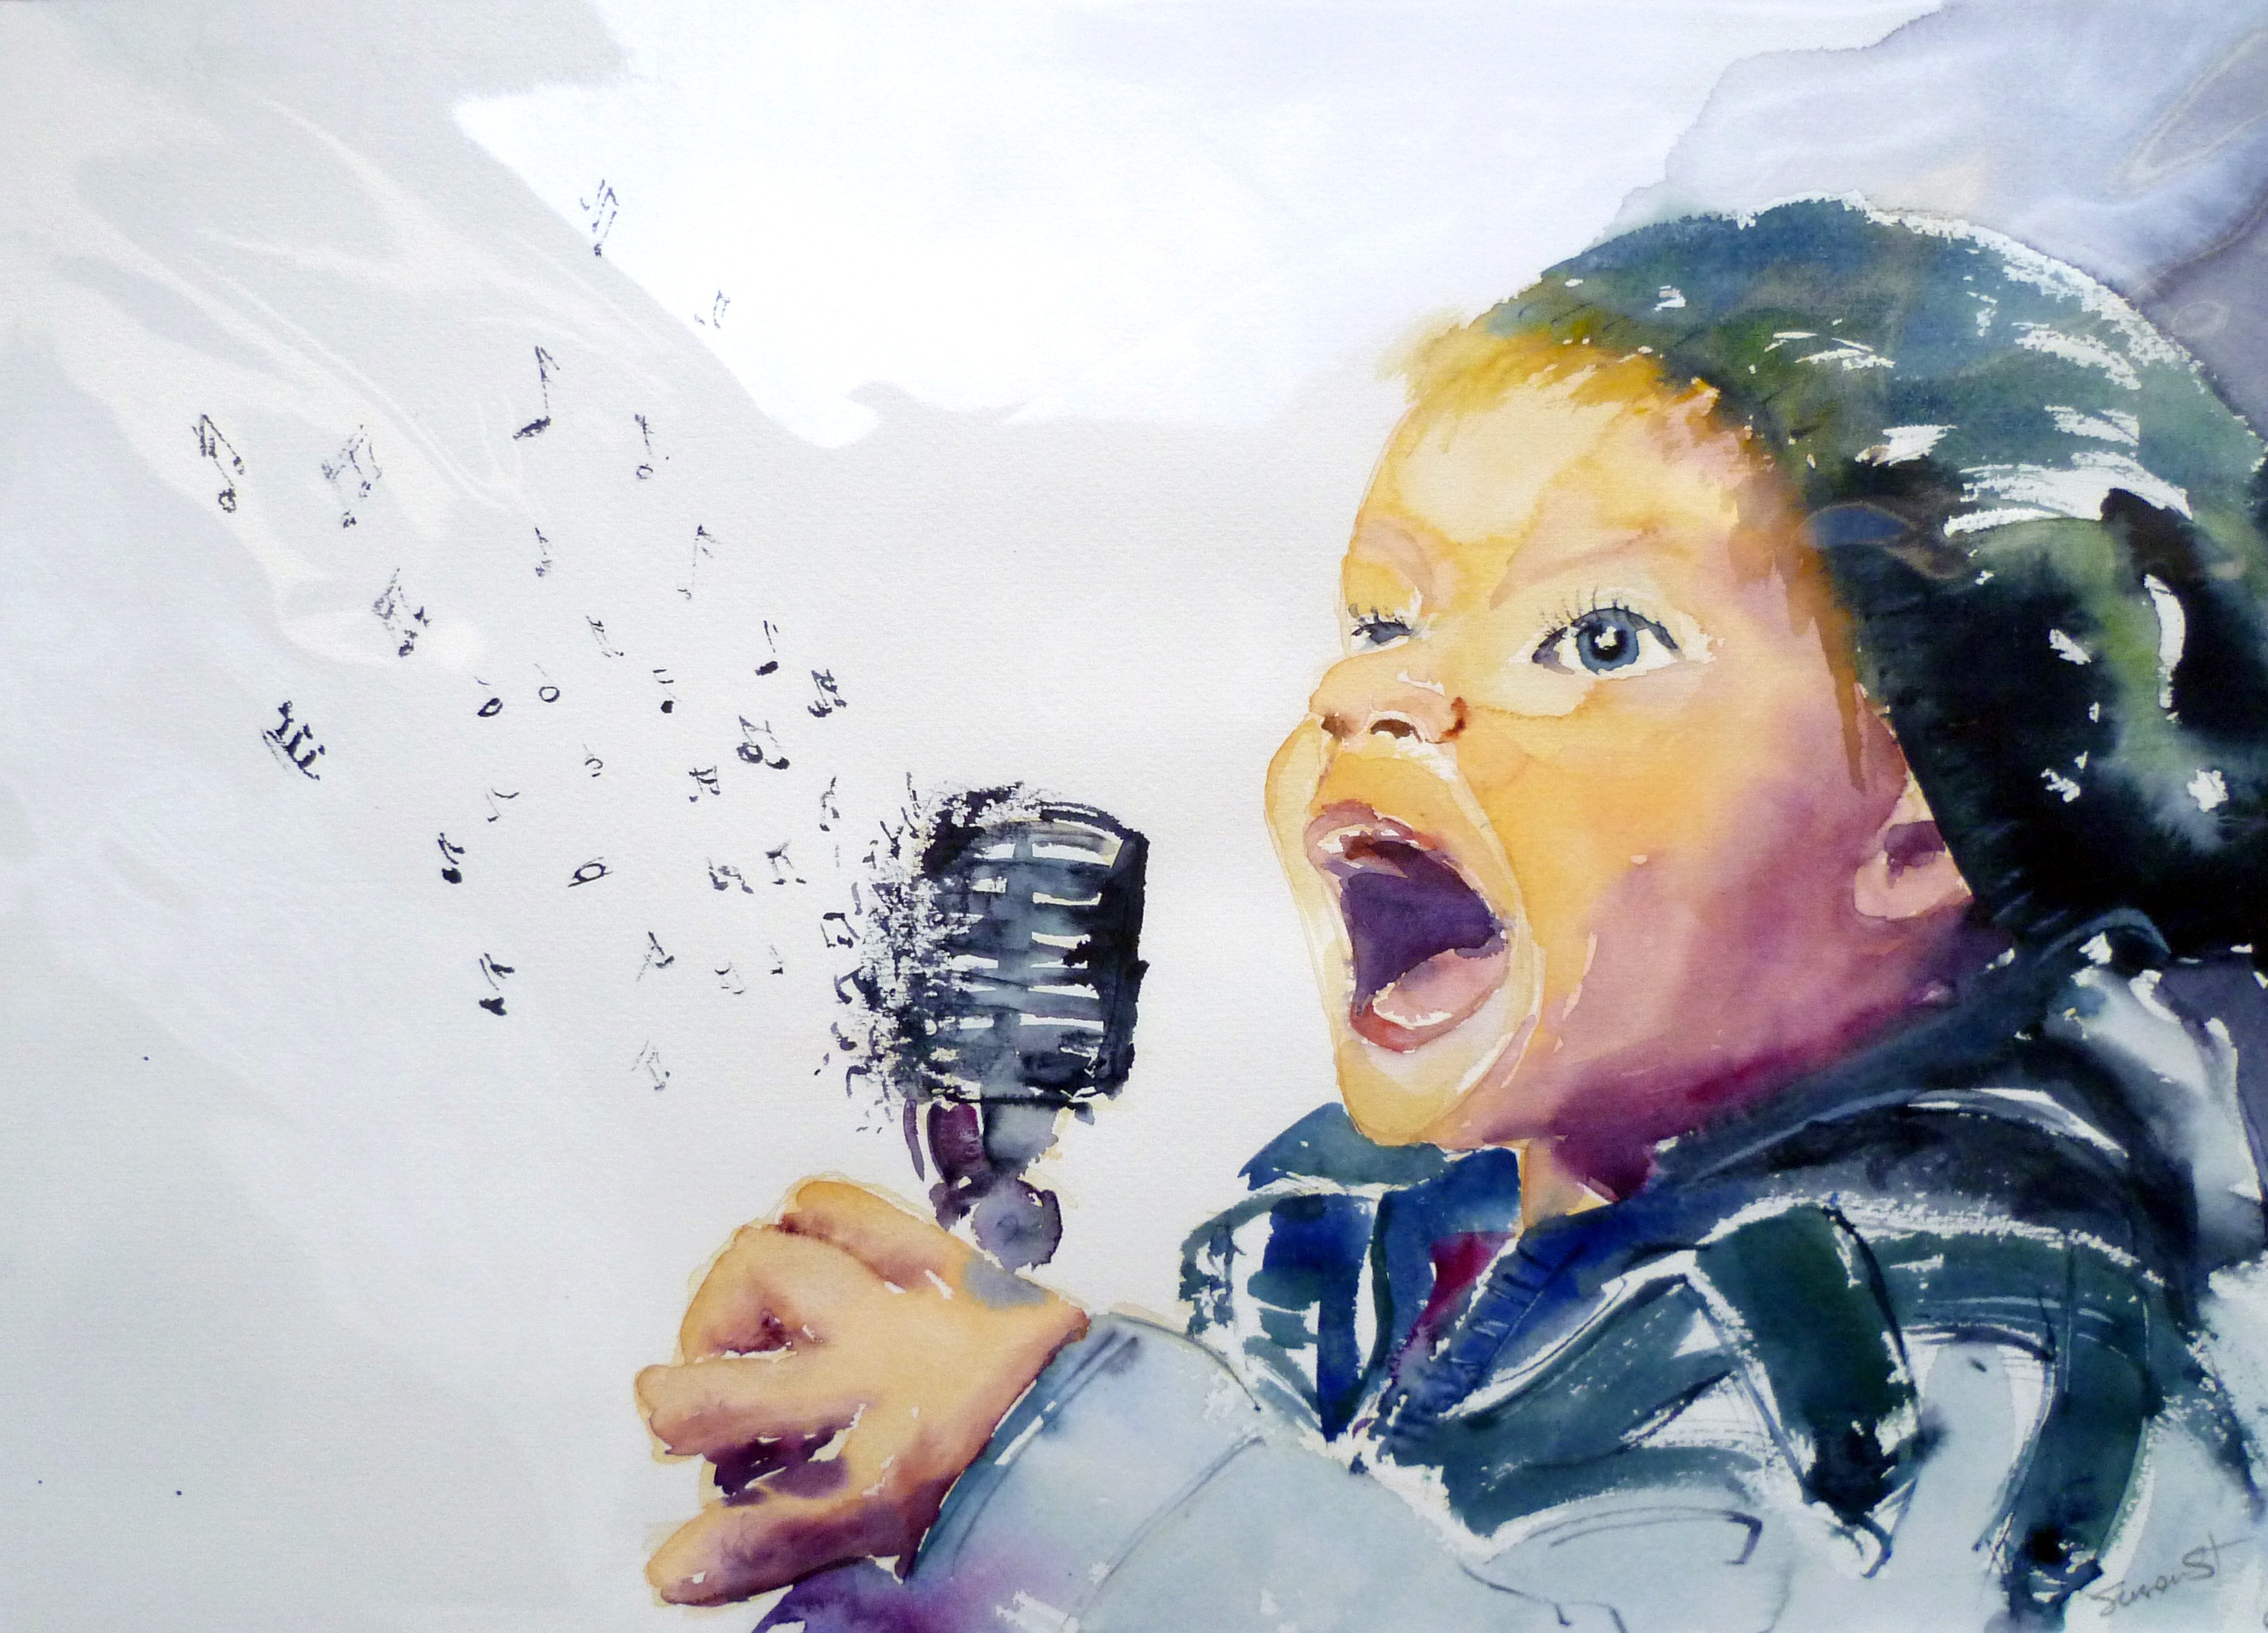
\includegraphics[width=\linewidth]{images/susanne/j10_lobtdenherrnmitallerkraft}\\

\vspace*{1mm}
\begin{center}

	\Large{\parbox{\linewidth}{
		\begin{center}
		{\Large
		\texttt{
			\textit{ Ich danke dir dafür,
        dass ich wunderbar gemacht bin; wunderbar sind deine Werke; das erkennt meine Seele. }
			}
		}
		\end{center}
		\begin{center}
		{\Large
			\texttt{{\textemdash Psalm 139,1}}
		}
		\end{center}
	}
}
\end{center}

\end{center}


%pjesma 11
\newpage
\phantomsection
\begin{minipage}[b]{0.5\linewidth}
\addcontentsline{toc}{section}{\texorpdfstring{{\rednifont\doccolor11.}\hspace{\twodigitspacing}}{}FREUE DICH SEHR \ttfamily(Sach 9,9)}
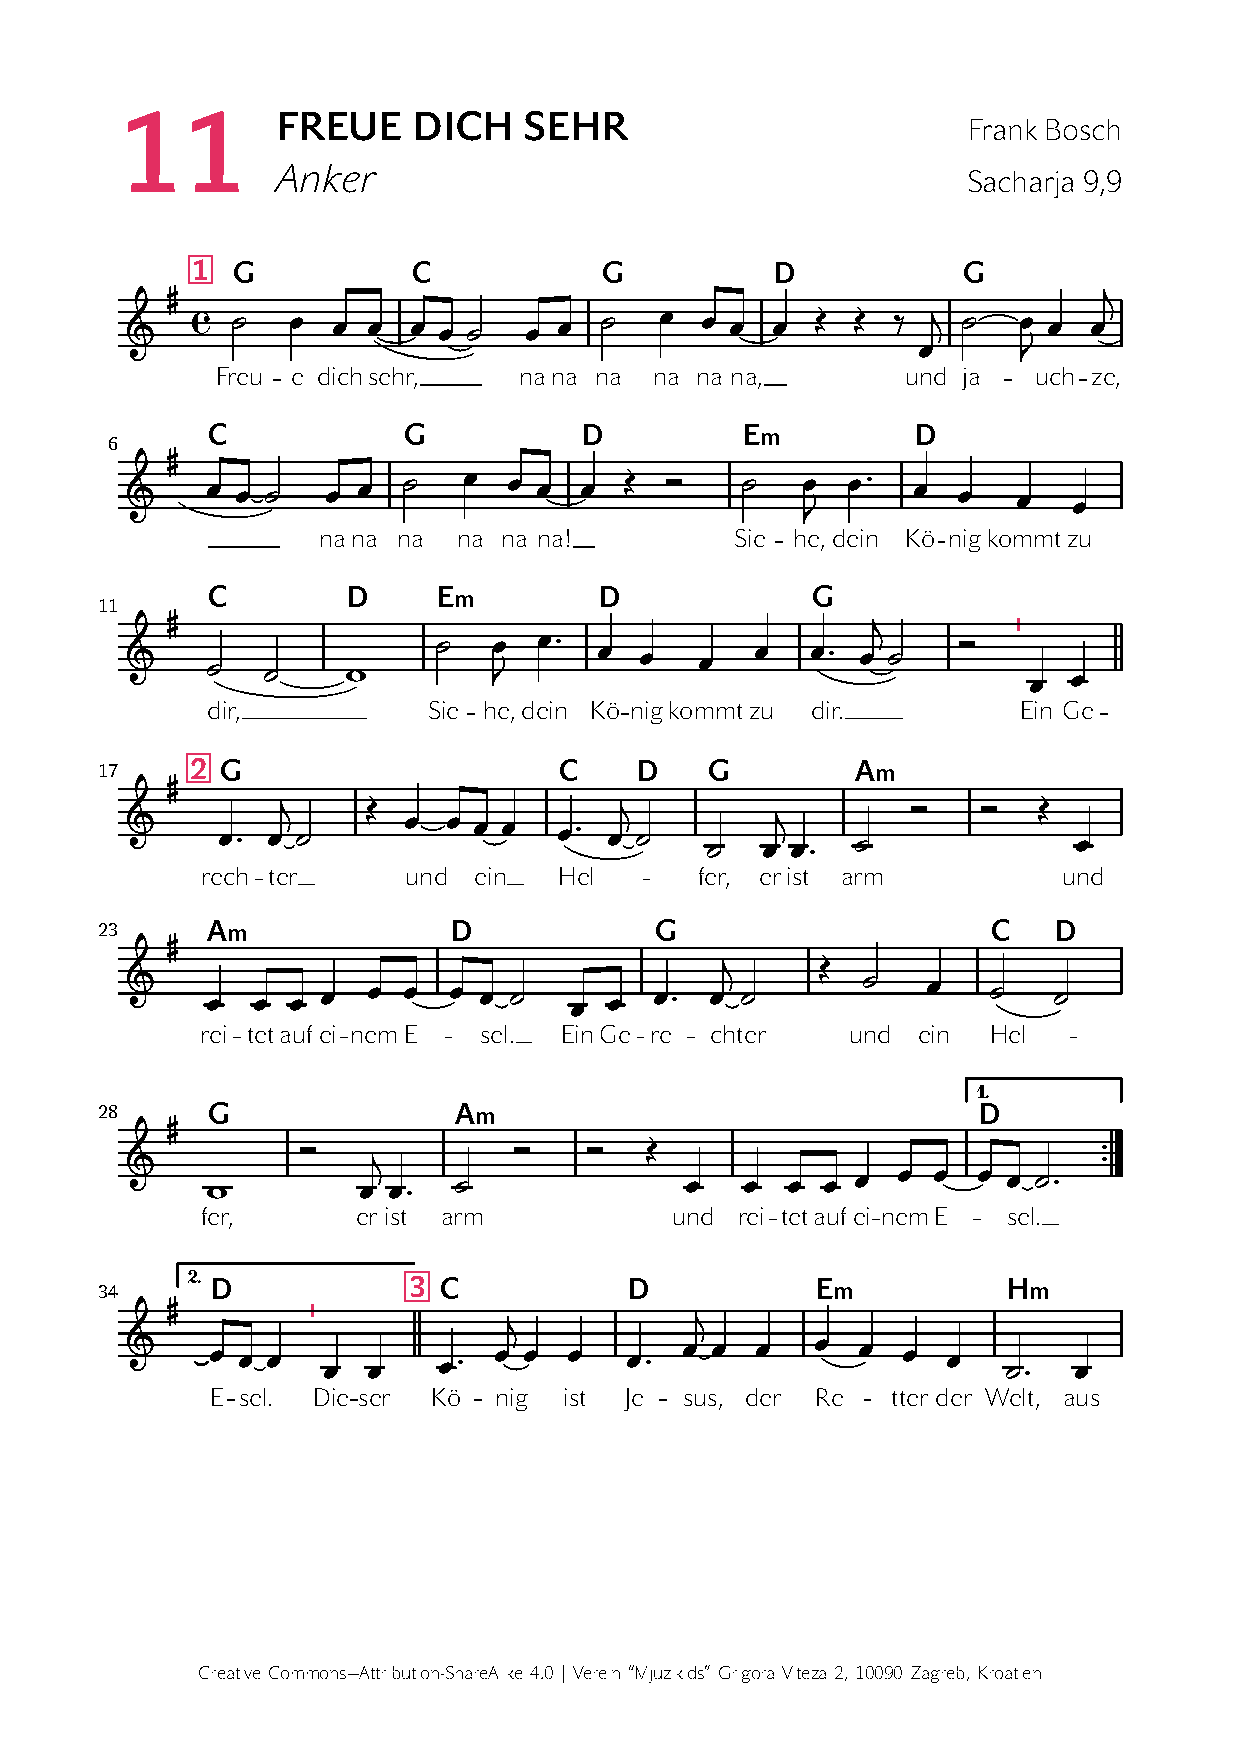
\includepdf[pages={1},noautoscale]{lilypond/de/src/11_freue_dich_sehr.pdf}
\end{minipage}

\newpage

\includepdf[pages={2},noautoscale, %
    picturecommand={\setlength\unitlength{1cm}%
         \put(2,5){\includegraphics[width=\linewidth,scale=1]{images/susanne/k11_freuedichsehr}}}]%
         {lilypond/de/src/11_freue_dich_sehr.pdf}

%pjesma 12
\newpage
\phantomsection
\begin{minipage}[b]{0.5\linewidth}
\addcontentsline{toc}{section}{\texorpdfstring{{\rednifont\doccolor12.}\hspace{\twodigitspacing}}{}SINGT DEM HERRN \ttfamily(Ps 96,1–3.10)}
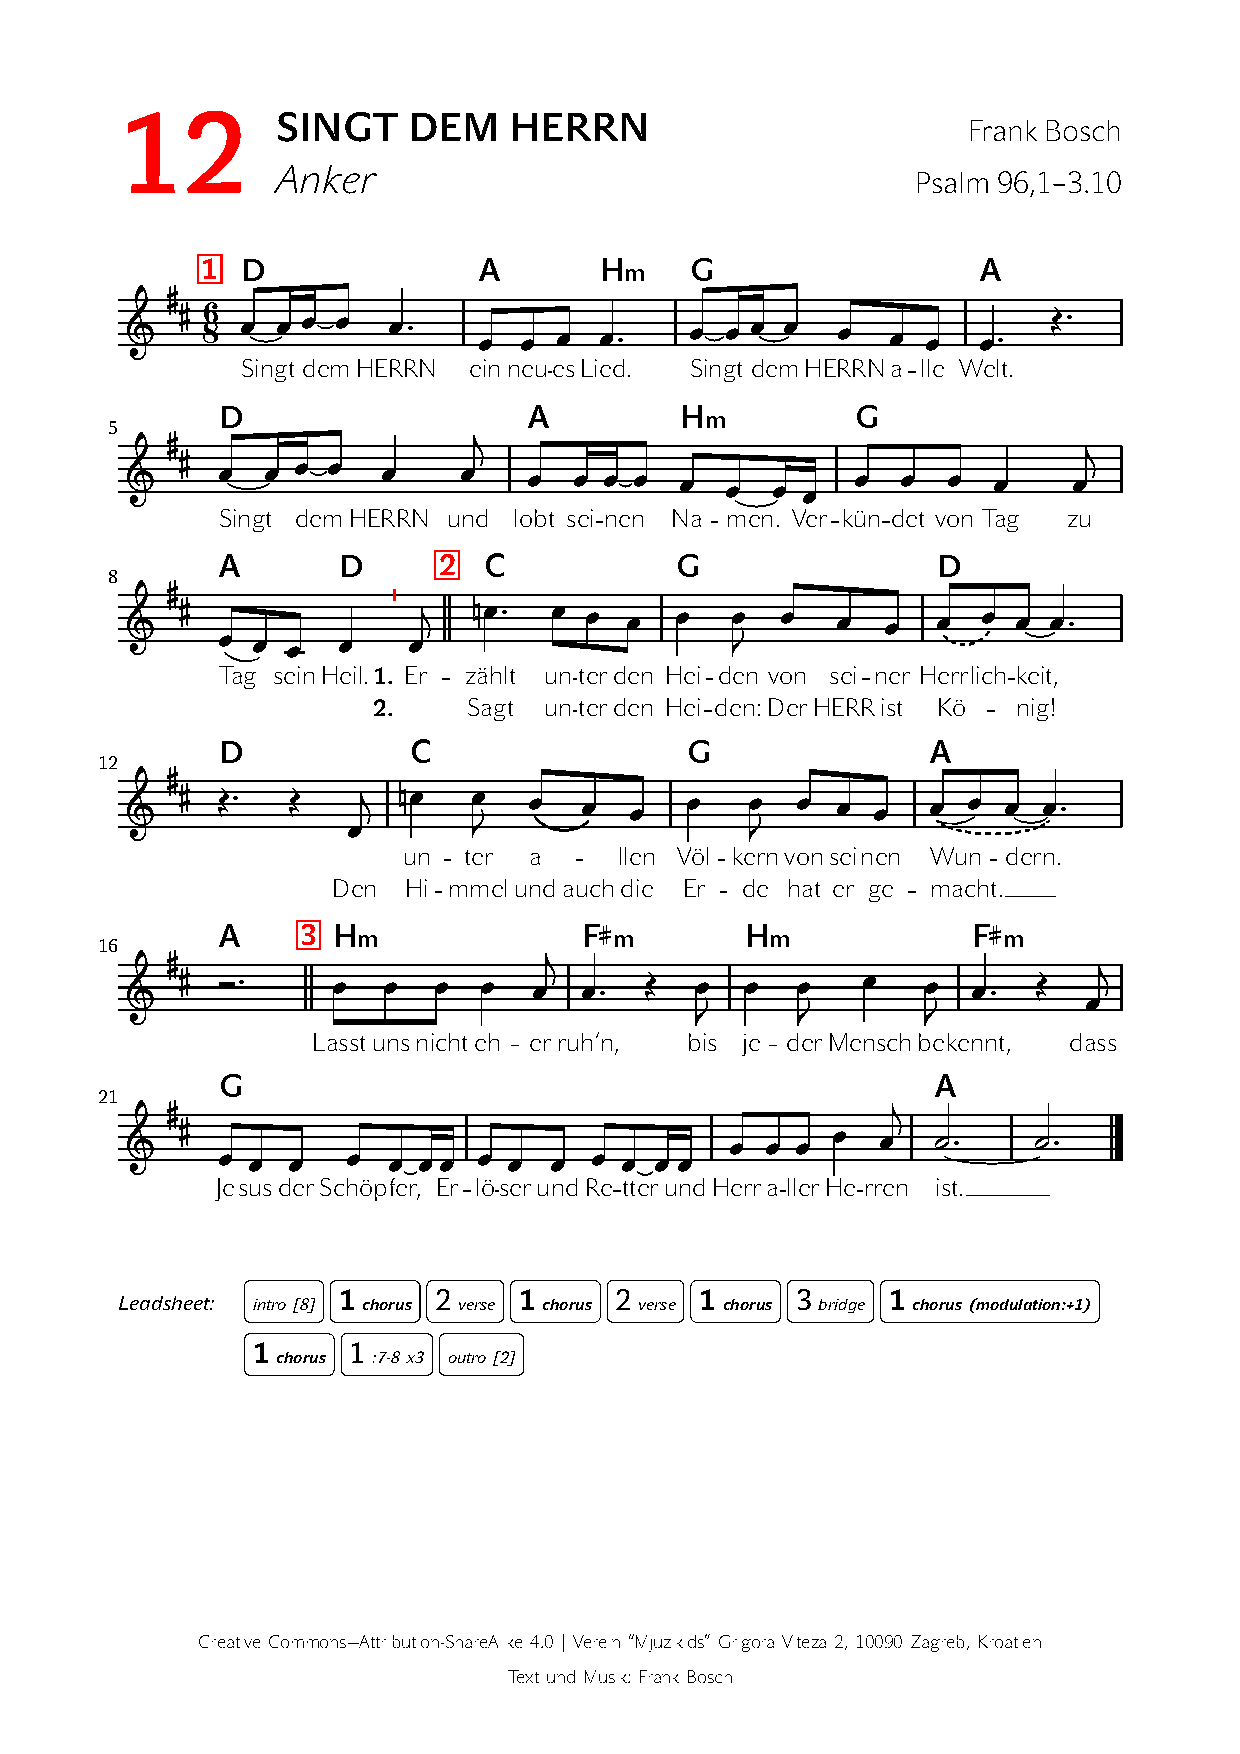
\includepdf[pages={1},noautoscale]{lilypond/de/src/12_singt_den_herren.pdf}
\end{minipage}

\newpage
\begin{center}
\includegraphics[width=0.95\linewidth]{images/susanne/l12_singtdemherrn}\\
\vfill
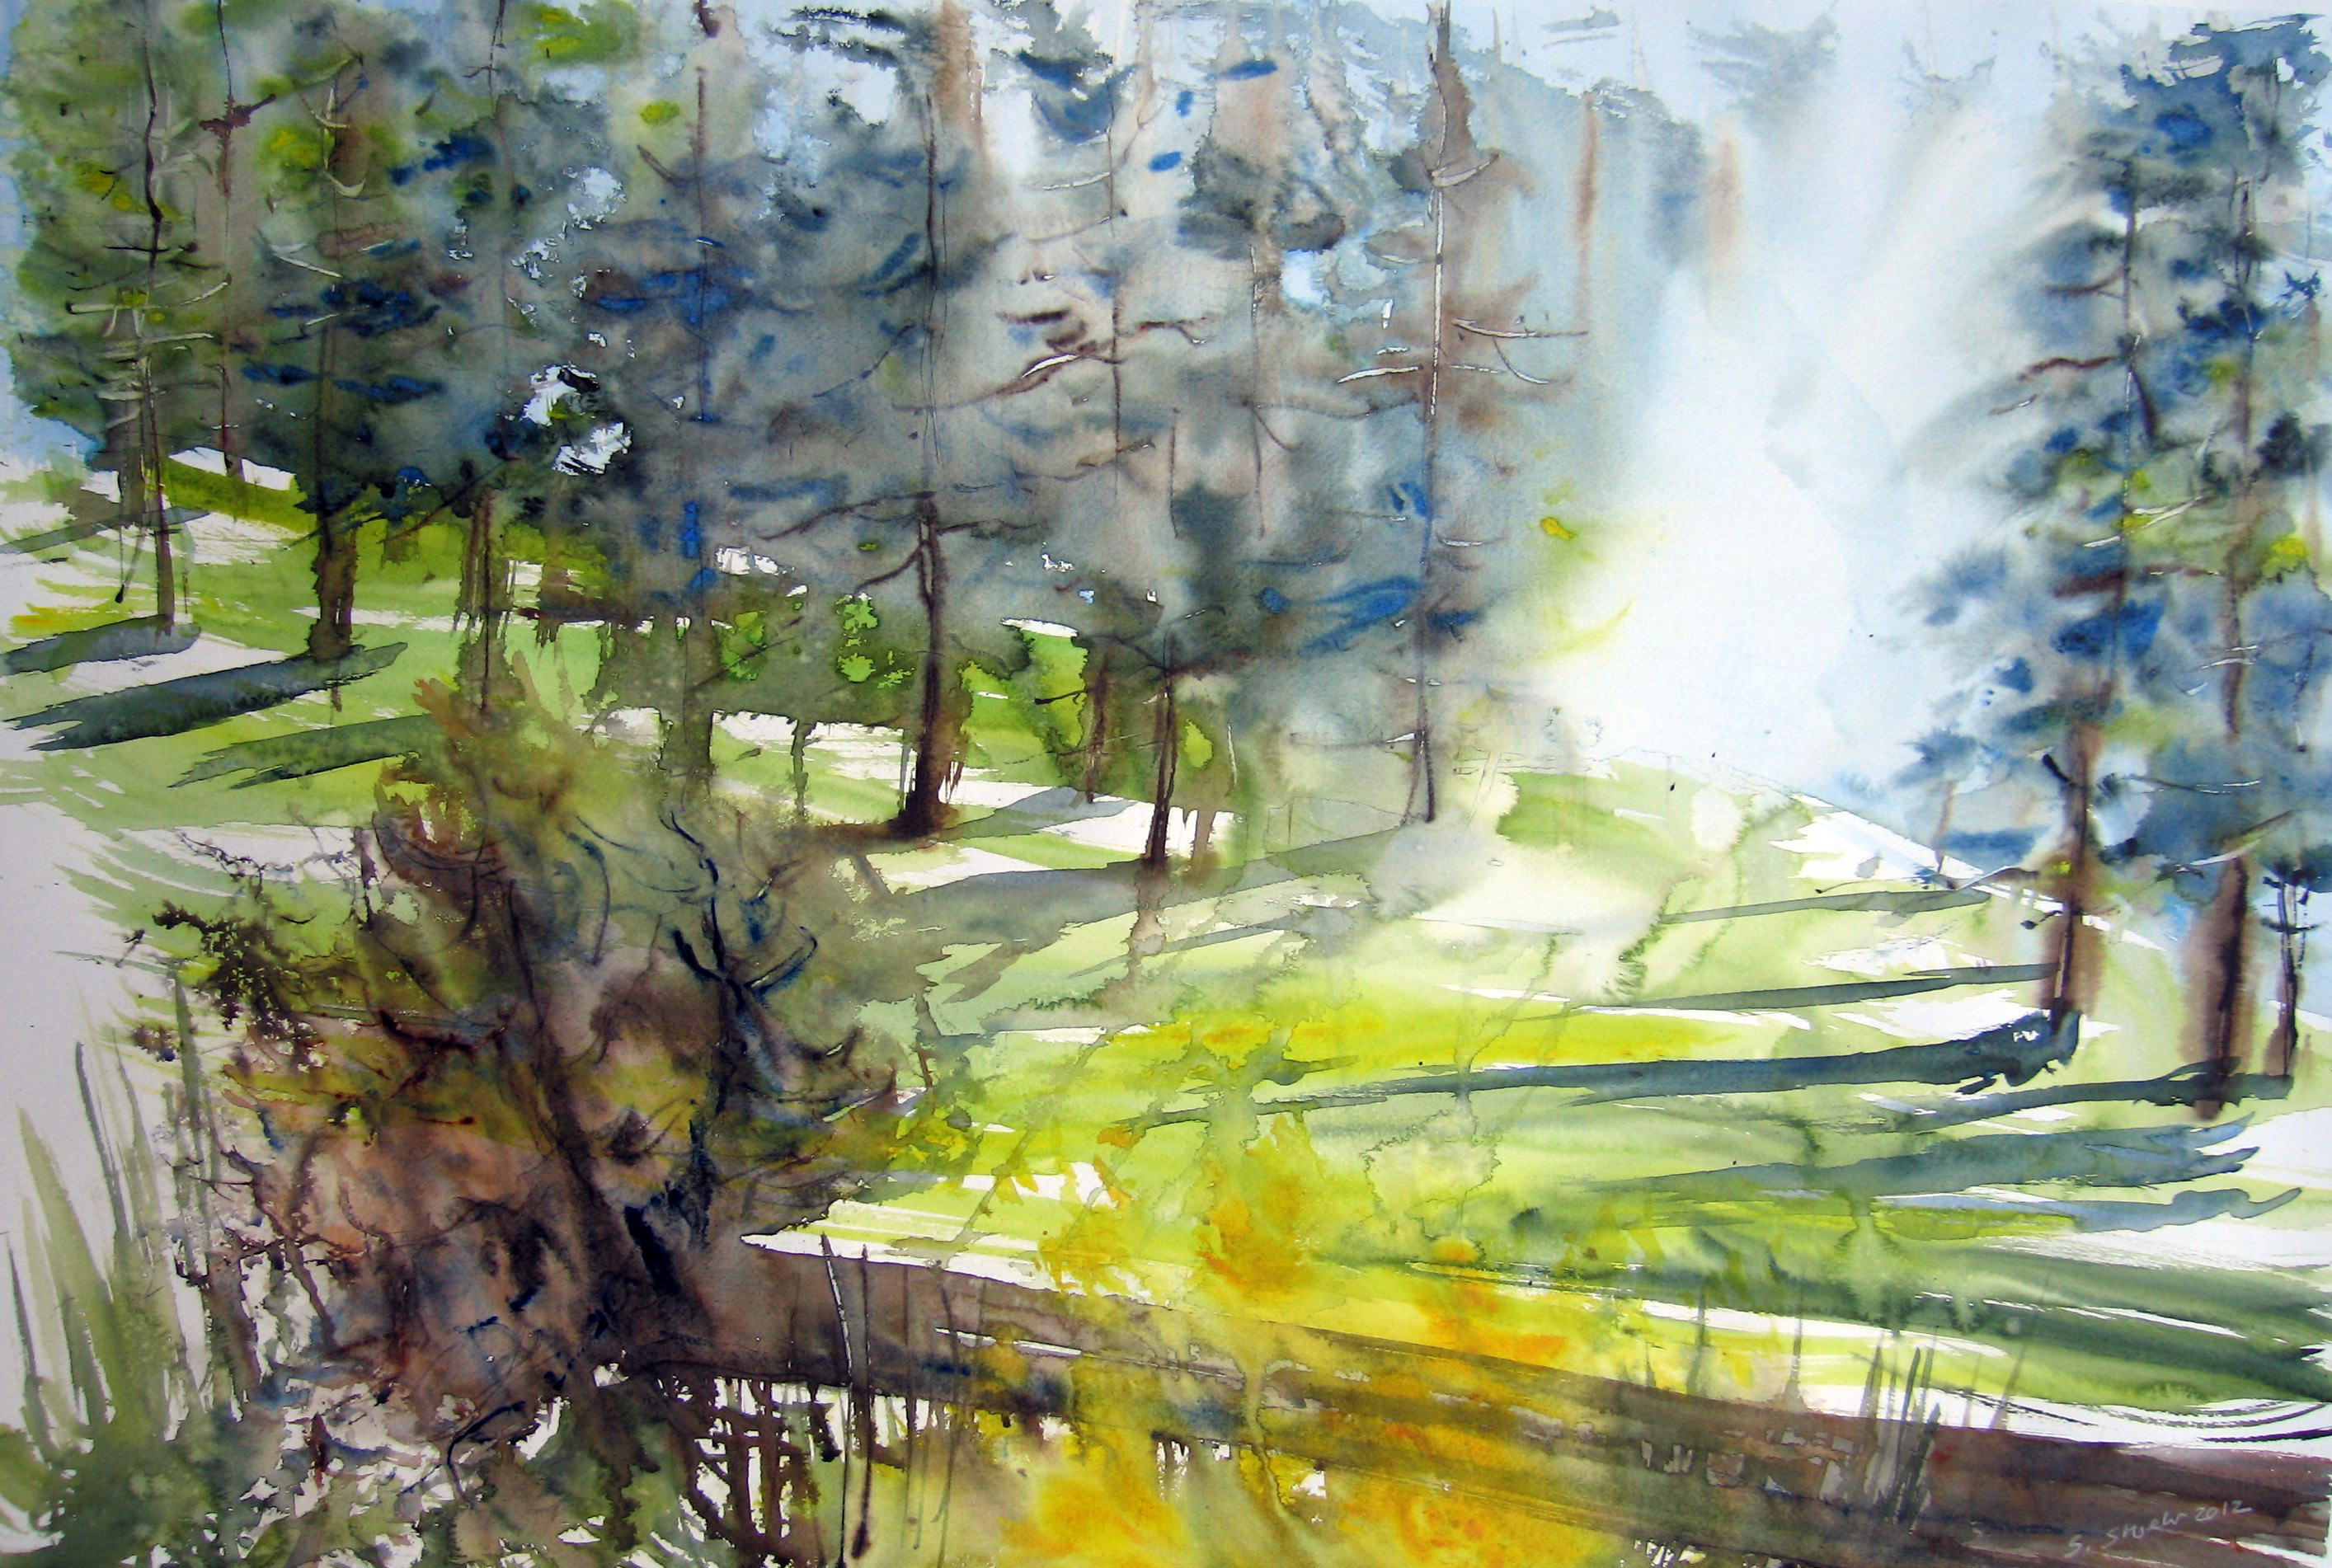
\includegraphics[width=0.95\linewidth]{images/susanne/a1_gedankendesfriedens}
\end{center}

\end{document}
%#################################################################################
%   END OF DOCUMENT
%#################################################################################